%Document vide aux normes de l'École nationale des Chartes
%crée par J.B. Camps
%Dernières modifications E. Rouquette (03/2026)

%%%%% PRÉAMBULE %%%%


	%%% partie obligatoire du préambule%%%
	
	\documentclass[12pt,twoside, openany]{book} % J'utilise openany pour que chaque partie et chaque chapitre ne commence pas forcément sur une page impaire. C'est très commode quand on imprime un document mais je trouve que pour un document que nous devons envoyer numérique, c'est gênant. 
	\usepackage{fontspec}
	\usepackage{xunicode}
	\usepackage{polyglossia}
	\setmainlanguage{french}%indiquer la langue principale du document
	%\setotherlanguage{} %indiquer les autres langues utilisée


%%%% PACKAGES UTILISÉS %%%%

	%%% Mise en forme %%%

		\usepackage{csquotes} % les guillemets français
		\usepackage{lettrine} %faire une lettrine (pas obligatoire)
		
		%charger le style de l'EnC (téléchargeable ici https://ctan.org/pkg/biblatex-enc)
		\usepackage[style=enc,sorting=nyt,maxbibnames=10]{biblatex}
		\addbibresource{./bibmemoire.bib} %le fichier bibliograhique. Exemple de chemin à partir du dossier où se trouve le document maître:Exemple ./dossierA/fichier.bib
		\defbibheading{stylebib}{\subsection*{#1}} %Si l'on veut changer le titre de la/les bibliographie(s)
		
	%%% Non utilisés %%%

		%%%Faire un ou plusieurs index
		%\usepackage{imakeidx} %pour faire un ou plusieurs index
		%\makeindex %commande pour générer l'index

	%%% Packages personnels %%%

		\usepackage{graphicx} % Insérer des images
		\usepackage{float} % Permet un plus grand contrôle sur les objets (tables, images etc...)}
		\usepackage{caption} % Permet la modification de la mise en page des légendes.
		\usepackage{pdfpages} %Permet d'ajouter un pdf
		\usepackage{enumitem} % changer l'interligne entre les items de itemize


%%%% CONFIGURATION DE MISE EN PAGE %%%%

	%%% Les compteurs (sections, subsections, etc) %%%

		\renewcommand{\thesection}{\Roman{section}.} %On ne fait apparaître que le numéro de la section
		\renewcommand{\thesubsection}{\arabic{subsection}.} %subsection en chiffres arabes
		\renewcommand{\thesubsubsection}{\alph{subsubsection}.}	%subsubsection en lettres minuscules
		%Si l'on veut faire apparaître les subsubsection dans le table des matières (à commenter sinon)
		\setcounter{tocdepth}{3}
		\setcounter{secnumdepth}{3}  % La subsubsection (profondeur=3 dans la table des matières) apparait numérotée dans la table des matières
		\counterwithout{footnote}{chapter} % Pour ne pas recommencer le compteur de notes de bas de page à chaque section et chapitre. 

	%%% Configurer le document selon les normes de l'école %%%

		\usepackage[margin=2.5cm]{geometry} %marges
		\usepackage{setspace} % espacement qui permet ensuite de définir un interligne
		\onehalfspacing % interligne de 1.5
		\setlength\parindent{1cm} % indentation des paragraphes à 1 cm


	%%% Mise en forme des headers (haut de page) %%%

		\usepackage{fancyhdr} %package utilisé pour modifier les headers
		\pagestyle{fancy} %utiliser ses propres choix de mise en page et non ceux par défaut du package

		\setlength\headheight{16pt}%la hauteur des headers

	%%% la façon dont les sections apparaissent dans les en-tête: %%%

		%\renewcommand{\sectionmark}[1]{\markright{\small\textit{\thesection~\  #1}}} %Faire apparaître dans les headers les sections en  petit et en italiques
		\renewcommand{\sectionmark}[1]{}%Commenter la ligne précédente et mettre celle-ci pour ne pas avoir le titre des sections dans le header

	%%% réglages propres à frontmatter %%%

		\appto\frontmatter{\pagestyle{fancy}%
		\renewcommand{\chaptermark}[1]{\markboth{\small\textit{#1}}{}}% ne pas faire apparaître de <<numéro>> de chapitre dans les chapitres non numérotés (front: l'introduction, les remerciements, etc)
		}

	%%% réglages propres à mainmatter %%%

		\appto\mainmatter{
		\renewcommand{\chaptermark}[1]{\markboth{\small\chaptername~\thechapter~--\ \textit{#1}}{}}%faire apparaître dans les headers les sections en  petit et en italiques
		%\renewcommand{\chaptermark}[1]{}%Commenter la ligne précédente et mettre celle-ci pour ne pas avoir le titre des chapitres  dans le header
		}	

	%%% réglages propres aux annexes %%%

		\appto\appendix{
			\renewcommand{\chaptermark}[1]{\markboth{\small~Annexe \thechapter~--\ \textit{#1}}{}}%faire apparaître dans les headers le nom des annexes
			%\renewcommand{\chaptermark}[1]{}%Commenter la ligne précédente et mettre celle-ci pour ne pas avoir le titre des chapitres  dans le header
		}

	%%% Règlages d'hyphénation %%%

		%indiquer des règles d'hyphénation pour des mots précis si besoin
		%\begin{hyphenrules}{french}
		%	\hyphenation{}
		%\end{hyphenrules}
		
	%%% Réglagles personnels %%%
	
		\setlist[itemize]{noitemsep, topsep=2.5pt} % Définit les paramètres de mes listes

%%%% Package hyperref %%%%

	% A mettre après les autres appels de packages car redéfinit certaines commandes).
	
	\usepackage[colorlinks=true, linkcolor=black, filecolor=black, urlcolor=black, citecolor=black, breaklinks=true, pdfusetitle, pdfsubject ={Mémoire TNAH}, pdfkeywords={Institutions patrimoniales, Institut National de l'audiovisuel, Base de données, dépôt légal, documentation, datavisualisation, intelligence artificielle, découvrabilité}]{hyperref} %
	
	\usepackage[numbered]{bookmark}%va avec hyperref; marche mieux pour les signets. l'option numbered: les signets dans le pdf sont numérotés
	
	% Compléter pdfsubjet et pdfkeywords
	%Explication des options de hyperref (modifiables)
	% hyperindex=false
	% colorlinks=false: pour que le cadre des liens n'apparaisse pas à l'impression
	% breaklinks permet d'avoir des liens allant sur pusieurs lignes
	%pdfusetitle: utiliser \author et \title pour produire le nom et le titre du pdf
	
%%%% Package glossaries %%%%

	%Exception: il faut le charger APRÈS hyperref
	\usepackage[toc=true]{glossaries}
	\makeglossaries
	%avec TexStudio: F9 pour compiler le glossaire (s'il y a aussi un index)
	
	%mettre les entrées du glossaire ici ou les mettre dans un fichier à part que l'on appelle ici par \loadglsentries{nom_du_fichier.tex}
	\loadglsentries{./annexes/glossaire.tex}
	
	%Structure d'une entrée de glossaire
	%\newglossaryentry{}{%
	%	name={},%
	%	description={}
	%}


%%%% DÉFINITION DES COMMANDES ET ENVIRONNMENTS %%%%

	%Bloc de citation
	%COMMENTER
	\newenvironment{miseenavant}
	{
		\begin{list}{}{
				\setlength{\rightmargin}{0pt}
				\setlength{\listparindent}{0pt}
				\setlength{\itemsep}{0pt}
				\setlength{\parsep}{0pt}
			}
			\item\relax\itshape
		}
		{
		\end{list}
	}


%%%% INFORMATIONS POUR LA PAGE DE TITRE %%%%
 
\author{Mélina \textsc{Franot} - M2 TNAH}
\title{Titre du mémoire}

%%%% DOCUMENT
\begin{document}
	\begin{titlepage}
		\begin{center}
			
			\bigskip
			
			\begin{large}				
				ÉCOLE NATIONALE DES CHARTES\\
				UNIVERSITÉ PARIS, SCIENCES \& LETTRES
			\end{large}
			\begin{center}\rule{2cm}{0.02cm}\end{center}
			
			\bigskip
			\bigskip
			\bigskip
			\begin{Large}
				\textbf{Mélina Franot}\\
			\end{Large}
		%selon le cas
			\begin{normalsize} \textit{diplômée de licence langues littératures et civilisations étrangères et régionales parcours anglais et de licence d'histoire de l'art et archéologie}\\
			\end{normalsize}
			
			\bigskip
			\bigskip
			\bigskip
			
			\begin{Huge}
				\textbf{Accéder aux collections patrimoniales numériques}\\
			\end{Huge}
			\bigskip
			\bigskip
			\begin{LARGE}
				\textbf{Un défi pour les institutions alors que de nouveaux modes de consultation rencontrent des pratiques documentaires héritées}\\
			\end{LARGE}
			
			\bigskip
			\bigskip
			\bigskip
			\begin{large}
				Sous la direction de \textbf{Axel Roche-Dioré}
			\end{large}
			\vfill
			
			\begin{large}
				Mémoire 
				pour le diplôme de master \\
				\enquote{Technologies numériques appliquées à l'histoire} \\
				\bigskip
				2026
			\end{large}
			
		\end{center}
	\end{titlepage}

	\thispagestyle{empty}	
	\cleardoublepage
	
\frontmatter

	\chapter{Résumé}
\medskip
	\textbf{Français :} Avec ses plus de 28 millions d'heures au titre du dépôt légal, l'INA est une référence en matière de collecte, de conservation et de communication des productions audiovisuelles et télévisées. Ses collections numérisées brillent par leur abondance et leur omniprésence sur les réseaux sociaux. Pourtant, l'accessibilité à ces collections est plus que jamais un enjeu à l'INA. Le responsable ? Un traitement documentaire qui a bénéficié de nombreuses années d'adaptations aux usages et aux besoins changeants des publics et qui, aujourd'hui, rend difficile l'exploitation de la totalité des collections de l'INA. Nous allons explorer ensemble les raisons de cette dérive et les outils nous permettant de renverser cet état de fait. \\
	
	\textbf{Anglais :} With over 28 million hours held under legal deposit, in a matter of collection, preservation and communication of televisions production archives, INA is a reference. Its digitized collections stand out for their considerable volume and their omnipresence on social media. Yet, accessing this collection is more of a challenge than ever before. The culprit ? Documentary cataloging and indexing methods that has been adapted to the changing uses and needs of audiences, and which today makes it difficult to make full use of INA's collection. Together, we will explore the reasons behind this drift and the tools that will allow us to reverse it.\\
	
	\textbf{Mots-clés:} Institutions patrimoniales; Institut National de l'audiovisuel; Base de données; dépôt légal; documentation; datavisualisation; intelligence artificielle; découvrabilité
	
	\textbf{Informations bibliographiques:} Mélina Franot, \textit{Accéder aux collections patrimoniales numériques. Un défi pour les institutions alors que de nouveaux modes de consultation rencontrent des pratiques documentaires héritées}, mémoire de master \enquote{Technologies numériques appliquées à l'histoire}, dir. Axel Roche-Dioré, École nationale des chartes, 2026.
	
		\newpage{\pagestyle{empty}\cleardoublepage}
	
	\chapter{Remerciements}
	
\lettrine{T}ous mes remerciements à mon tuteur de stage Emmanuel Pije pour son accompagnement dans la découverte de cette grande institution qu'est l'INA. À mon tuteur de mémoire Axel Roche-Dioré pour son encadrement dans la rédaction de ce travail. Mes remerciements vont également à tous mes collègue de l'INA qui m'ont soutenu et accompagné dans la rédaction de ce mémoire et à mes camarades de classe de l'École nationale des chartes pour leur solidarité durant ces deux années de master. Sans oublier ma responsable pédagogique Emmanuelle Bermès pour toujours soutenir et représenter tous les étudiants de ce master \enquote{Technologies numériques appliquées à l'histoire}. À ma famille pour leur soutien et à mes parents pour m'avoir donné toutes les chances de réussir. Et enfin un grand merci à mes amis et plus particulièrement à Juliette pour avoir relu toutes les productions académiques que je lui ai jamais soumis. 
	\newpage{\pagestyle{empty}\cleardoublepage}
	
%%%%%%%%%%%% \bibliographie ici (normes de l'EnC)

	\chapter{Bibliographie}
	\markboth{\small\textit{Bibliographie}}{} % Je marque manuellement les headers parce que comme ma partie \enquote{Bibliographie} n'est pas notée, elle ne s'affiche pas non plus dans le header. 
	
	\printbibliography[heading=stylebib, keyword=histoire_patrimoine, title={Histoire et patrimoine}]
	
	\printbibliography[heading=stylebib, keyword=TD, title={Catalogage et traitement documentaire}]
	
	\printbibliography[heading=stylebib, keyword=ina, title={Institut National de l'Audiovisuel}]
	
	\printbibliography[heading=stylebib, keyword=archives, title={Archives}]
	
	\printbibliography[heading=stylebib, keyword=numerique, title={Numérique et documents}]
	
	\printbibliography[heading=stylebib, keyword=donnees, title={Données}]
	
	\printbibliography[heading=stylebib, keyword=expe, title={Expérience Utilisateur}]
	
	\printbibliography[heading=stylebib, keyword=loi, title={Textes de loi}]
	
	\printbibliography[heading=stylebib, keyword=site_web, title={Sites web}]
	
	\printbibliography[notkeyword=loi, notkeyword=ina, notkeyword=histoire_patrimoine, notkeyword=TD, notkeyword=archives, notkeyword=numerique, notkeyword=donnees, notkeyword=mediation_donnees, notkeyword=site_web, notkeyword=expe, title={Documents sans étiquette}] % Pour vérifier qu'il n'existe pas des citations auxquelles j'ai oublié de mettre une étiquette. 
	
\newpage{\pagestyle{empty}\cleardoublepage}
	
\chapter{Introduction}	

%% Incipit %%

Le 30 mai 2023, Gallica fêtait son dix millionième document numérisé\footcite[]{gallica10}. Exposant par la même occasion le succès de la numérisation des documents patrimoniaux, alors que 23 ans auparavant, elle peinait toujours à trouver sa place dans des institutions de conservation comme la BNF. Aujourd'hui cette numérisation est devenue indissociable de la communication des ces documents au plus grand nombre. Pourtant, une des conséquences de cette numérisation en masse est l'effacement de certains de ces documents parmi ces quantités de documents massive. En l'absence d'une représentation physique, il revient à ces institutions de mettre en place les outils nécessaires à la réalisation de leur mission de communication des collections patrimoniales dont ils ont la responsabilité. Ils disposent pour cela de nombreuses années d'expérience à documenter leur collection dans un objectif de communication. Malheureusement pour eux, cette numérisation est seulement un des témoins des bouleversements provoqués par l'informatisation de notre société. Les attentes des publics ont changé et une adaptation est nécessaire. 

%% Introduction INA %%

C'est dans ce contexte propices aux réflexions sur la communication de ces documents que prend place notre stage à l'Institut National de l'audiovisuel. Né de la dissolution de l’ORTF en 1974, l’Institut National de l’Audiovisuel, abrégé INA, est aujourd’hui une institution majeure de la conservation du patrimoine français. Pourtant, à sa naissance, il réunissait les oubliés de la dissolution avec l’archivage, la formation, la production de création et la recherche\footcite[][3]{hoog2006}. Depuis sa création, l’institut a conservé toutes ses missions d’origine mais s’est vu transformé par plus de 50 ans de mutation des institutions patrimoniales ainsi que de la définition même de la notion de « patrimoine », auquel l’audiovisuel s’est progressivement greffé. Porte étendard de ces évolutions à l’INA, la loi du dépôt légal du 20 juillet 1992 grâce à laquelle l’institution intègre deux nouvelles missions : la conservation patrimoniale et la communication à des fins scientifiques\footcite{fillioud1994}. D’un autre côté, en matière de changements, le paysage télévisuel n’est pas en reste non plus. Les chaînes se multiplient, les contenus se diversifient, l’INA a adapté son fonctionnement à ces évolutions. A titre général, le monde s’est progressivement informatisé, ce qui permis au grand public de se rapprocher de ses archives audiovisuelles grâce à des plateformes comme ina.fr\footcite{zotero-item-158} alors que les professionnels de l’INA, eux, perdent le contact avec les supports analogiques pour l’immatérialité de la donnée\footcite[][68]{bassaïstéguy2025}. Aujourd’hui professionnel de l’INA ou grand public, tous accèdent aux documents par les données qui leur sont associées\footcite[][118]{alquier2017}. En cela le \gls{td} réalisé de ces documents tient une place importante dans leur communication à tous les publics. Des années durant, les politiques documentaires ont adapté leurs pratiques à ses usagers. La conséquence étant aujourd'hui que cette quantité massive de données est empreinte de tous les bouleversements d'ordre sociaux, économique ou technologiques au cours desquelles elle se construisait. A tel point où désormais, l'accessibilité aux collections des institutions patrimoniales est un véritable enjeu. 

%% Stage %%

C'est de ce constat que né le projet auquel j'ai pris part au cours de mon stage à l'institut national de l'audiovisuel. J'avais pour mission de participer aux réflexions sur la conceptualisation d'un outil permettant de rendre ces données moins opaques, plus loquaces afin de faciliter la découvrabilité des fonds et la recherche dans les bases de données de l'INA. Le \gls{td} de ces documents audiovisuels n'est pas égal, il est le résultat de multiples politiques documentaires, découlant d'un contexte spécifique, sans pour autant avoir laissé de trace de ces changements. En conséquent, la précision de ce \gls{td} varie selon la \gls{pd} en vigueur lors de son dernier traitement mais aussi selon un certain nombre de critères variables mais qui ne sont aucunement documenté non plus. C'est pourquoi ce projet vise à cartographier l'histoire du \gls{td} à l'INA. Parmi toutes les données que produit l'INA, ce sont à celles-ci que sont confronté les chercheurs et ce sont celles-ci qui déterminent la compréhension des collections de l'INA. Leur absence est aussi équivoque que leur présence. Ce projet ayant pour objectif de produire un outil permettant à différents publics de comprendre, explorer et exploiter les bases de données de l'INA, il nous a été essentiel de déterminer \textbf{en quoi l'évolution des pratiques documentaires au sein des institutions patrimoniales représente aujourd'hui un enjeu d'accessibilité aux collections ? Quels outils permettent d'adapter cet héritage à de nouvelles habitudes de consultation ?}

%% Plan %% 

Afin de répondre à cette question, nous procéderons en trois étapes. Premièrement nous analyserons les publics confrontés à ces collections patrimoniales et nous expliciterons à quels enjeux répond leur accessibilité. Une fois que nous aurons déterminer cela, nous parcourrons l'histoire du \gls{td} à partir de la naissance de cette institution afin de déterminer comment le \gls{td} en est arrivé à générer la situation précédemment décrite. Pour finir, nous utiliserons ce que nous aurons déduit de ces analyses afin de déterminer quels outils nous permettent d'adapter cette histoire du \gls{td} aux nouvelles habitudes de consultation de ces publics. 

%% Méthodologie %%

Cette analyse utilisera principalement des exemples issus de la situation actuelle du \gls{td} à l'institut national de l'audiovisuel desquels nous tenterons de tirer des conclusions générales sur des institutions patrimoniales issues du paysage patrimonial français, en prêtant une attention particulière aux institutions responsables de la mission du dépôt légal. Nous tirerons nos conclusions de l'analyse de la littérature scientifique, de notre expérience personnelle au sein de l'institution ainsi que de l’expérience de trois professionnels de l'INA exprimées dans trois entretiens semi-dirigés. Ils ont été sélectionnés afin de correspondre à trois profils de publics ciblés par les activités de l'INA ou concernés par le \gls{td} : les documentalistes avec une documentaliste ayant souhaité gardé l'anonymat, du service \enquote{Traitement et enrichissement des collections}, les chercheurs avec Arthur Hénaff, chef de service de l'INAthèque et enfin les professionnels de l'audiovisuel avec Pascal Lebeurier, cadre documentaire du service \enquote{Clients et partenaires}. 

%% Vocabulaire %%

Au cours de cet exposé nous utiliserons à plusieurs reprises le terme d' \enquote{archives} pour parler de documents audiovisuels conservés. Ce terme n'est pas utilisé au sens premier des archives comme le résultat d'une activité administrative ou juridique. Exit également la notion d'original, incompatible avec ces documents, majoritairement numériques pour lesquels la question d'original est très complexe. Nous utiliserons ici le terme d'\enquote{archives} comme un objet conservé et communiqué par une institution\footcite[Réflexion inspirée de l'article suivant][]{zotero-item-739}. 
%si l'introduction est longue, elle peut être importée avec input

\newpage{\pagestyle{empty}\cleardoublepage}

%%%%%%%%%%%%%%%%%Le corps du mémoire
	\mainmatter
%Trier par dossiers si besoin (front, main,annexes,), se crérer un docuemnt .tex par structure (section ou chapter selon la taille et la pertinence) Exemple de chemin à partir du dossier où se trouve le document maître: ./dossierA/fichier.tex

\part{Accessibilité aux collections patrimoniales}

%% Introduction - Le pourquoi du comment on dit ça %%

Le projet de cartographie du traitement documentaire réalisé à l'INA nécessite avant tout de comprendre les raisons de son existence afin de déterminer à quels besoins il doit répondre. En effet, ces collections sont au contact de plusieurs typologies de publics avec leurs propres pratiques, usages et besoins. Ils accèdent aux collections des institutions patrimoniales par des outils différents et ont en conséquent une expérience différente d'une typologie de public à l'autre. C'est pourquoi nous allons dans un premier temps poser les bases de notre réflexion en analysant ces enjeux de l'accessibilité aux collections patrimoniales. 

%% Plan %%

Dans ce sens, nous allons décrire et analyser les publics des institutions patrimoniales en les divisant en catégories de publics : le grand public, les chercheurs, les documentalistes et les professionnels de l’audiovisuel. Nous décrirons leurs habitudes, leurs pratiques et les outils à leurs dispositions avant de préciser, dans une seconde partie les différents freins à l'accessibilité qu'ils rencontrent. 

	\chapter{Nouveaux profils et nouvelles habitudes de consultation des collections}
	
		\section{Le grand public : le petit nouveau}
		
		%% Introduction %% 

Nous réunissons sous le terme de \enquote{grand public} toutes les populations ne possédant pas d'expertise, de connaissance ou de besoins vis-à-vis des institutions patrimoniales. Ce public couvre donc une population très large et pourtant, dans l'histoire des collections patrimoniales, cette typologie est toujours la dernière à avoir accès à ces collections. 

\subsection{Le dépôt légal, déclencheur de l'accessibilité aux collections patrimoniales}

%% Situer dans le temps %%

C'est le dépôt légal qui par nature, ouvre les collections patrimoniales à toutes les populations. A l'INA, avant sa mise en place, il n'était pas question, pour le grand public, d'avoir accès aux documents que l'institut de l'audiovisuel conservait. A vrai dire, il n'était pas question pour beaucoup de publics d'avoir accès aux images et sons. Comme en témoigne notre documentaliste interrogée. Avant les importants travaux de numérisation dans les années 2000, l'accès aux images et sons conservés par l'INA étaient restreints par leurs supports. En 1993, les documentalistes envoyaient leur commandes par fax aux magasins et ils constataient quelles images avaient été sélectionnées quand elles passaient à la télévision, en même temps que le grand public. Avec le dépôt légal et l'ouverture de l'INAthèque à la BNF François-Mitterand en 1995, le grand public a enfin accès aux diffusions télévisées conservées. 

Malgré tout, le dépôt légal ne signifie pas toujours de l'ouverture au grand public. En 1537, date de la création du dépôt légal des manuscrits, l'ouverture des collections de la bibliothèque royale reste restreinte et il faudra attendre 1720 et l'ouverture de la \enquote{Salle B} à la BNF pour voir une première ouverture à un public \enquote{non-savant}\footnote{Cours d'Initiation aux bibliothèques à l'époque contemporaine de M1 de Technologies numériques appliquées à l'Histoire dispensé par Christine Bénévent}. L'écart des publics au début du dépôt légal de la BNF et de l'INA ne sont certes pas comparables mais ils ont de commun qu'une ouverture au grand public ne signifie pas toujours que le grand public s'aventurera dans les collections de son institution. Les collections patrimoniales s'ouvrent avant tout à un public de chercheurs. En cela les avancées technologiques et leur généralisation dans la société ont contribué à l'ouverture de ces collections et de leur médiation à véritablement tous les publics. Grâce à la numérisation de ces documents et à la démocratisation de l'informatique personnel, les collections numériques des institutions patrimoniales s'invitent à domicile et plus récemment dans nos poches, grâce aux téléphones portables. 

\subsection{Sites web et réseaux sociaux : amener le patrimoine au grand public}

%% Sites web %% 

La principale porte d'entrée aux collections patrimoniales des institutions est la médiation en ligne de leurs collections. Cette ouverture commence par des sites web tels que Gallica\footcite{gallica} en 2000 ou ina.fr\footcite{ina} en 2006. Ces sites proposent une sélection de documents de l'institution, découpés et présentés pour le grand public\footcite[][136]{bermès2024} comme ouvertures aux collections tout en permettant la recherche. 
\begin{figure}[H]
	\centering
	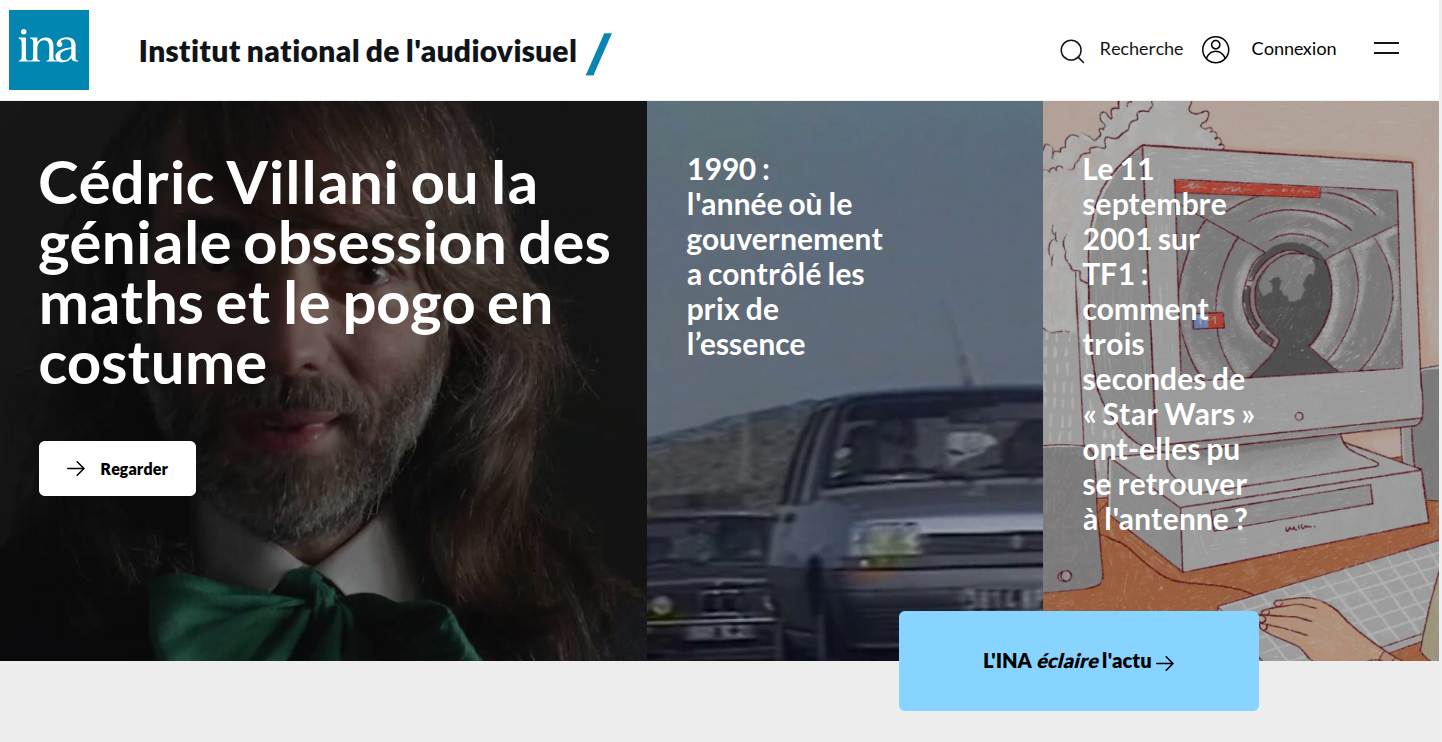
\includegraphics[width=0.75\textwidth]{./illustrations/inafr.png}
	\caption{Capture d'écran de l'accueil du site ina.fr}
	\label{fig:siteweb}
\end{figure}
Pour l'INA, c'est un grand succès, dès son lancement le site trouve son public, qui s'approprie directement les collections. Ils recherchent leurs souvenirs télévisés avec les shadoks, des moments forts de la télévision en cherchant le Général De Gaulle ou plus simplement en recherchant le moment fort de la télévision à la date de leur naissance\footcite[]{zotero-item-158}. 

%% Réseaux sociaux %%

Quelques années plus tard, ce sont avec les réseaux sociaux que ces institutions viennent à la rencontre du grand public. Ils adoptent les codes du web en s'adaptant aux formats courts des réseaux sociaux. En retour, les internautes s'approprient ces documents d'archives. En 2017 la \enquote{carte gastronomique} de la BNF, une carte gastronomique de la France établie par Alain Bourguignon en 1929 connaît un grand succès quand les internautes partagent leur spécialités culinaires locales en ligne sur les réseaux sociaux\footcite[][5]{bertrand2021/mars/15}. Sur les comptes de ces institutions, les équipes d'éditorialisation mettent en scène des évènements d'actualités afin de susciter des réactions chez ce public et à potentiellement susciter de l'intérêt à explorer le reste des collections afin de les rediriger vers des contenus qu'ils ne consulteraient pas spontanément. Récemment, on pouvait voir des utilisateurs des réseaux sociaux s'approprier et parodier les codes des documents de l'INA sur les réseaux\footnote{Les exemples évoqués ont été trouvés sur le réseau social Instagram avec les hashtags \enquote{ina} et \enquote{parodie}}. Dans la continuité des réseaux sociaux il existe un service de l'INA, nommé \enquote{Mediaclip}, un outil clef en main permettant aux créateurs de contenu d'acheter des extraits de documents de l'INA\footcite{zotero-item-708}. Désormais la majorité des institutions patrimoniales ont leur réseaux sociaux afin de toucher un public plus large. Cela comprend les musées comme le Louvre, le musée d'Orsay ou des centres d'archives et ce peu importe la taille de l'institution. Ils fait désormais partie des missions du \gls{td} de permettre de mobiliser ces documents. Par l'intermédiaire des réseaux sociaux, ces documents, quels qu'ils soient, peuvent être mobilisés pour éclairer l'actualité\footcite[][147]{caporiondo-prost2026}, comme l'illustrent ces captures d'écran de publications sur le réseaux social \enquote{Instagram} des archives nationales, de Gallica, du Louvre et de l'INA le 12 août 2026, jour d'éclipse.
\begin{figure}[H]
	\centering
	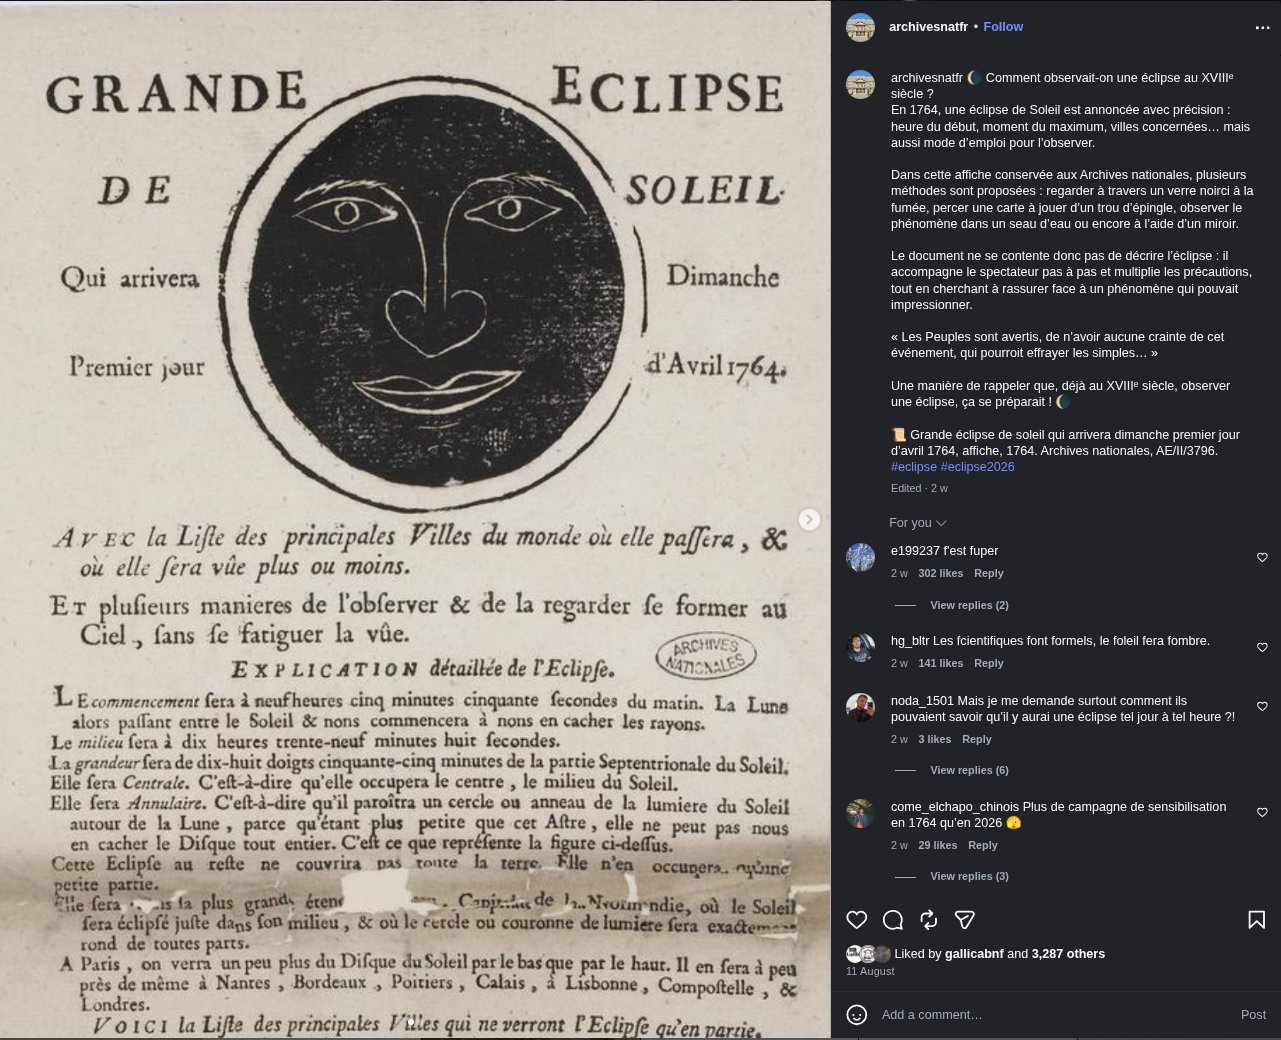
\includegraphics[width=0.24\textwidth]{./illustrations/insta_an.png}\hfill
	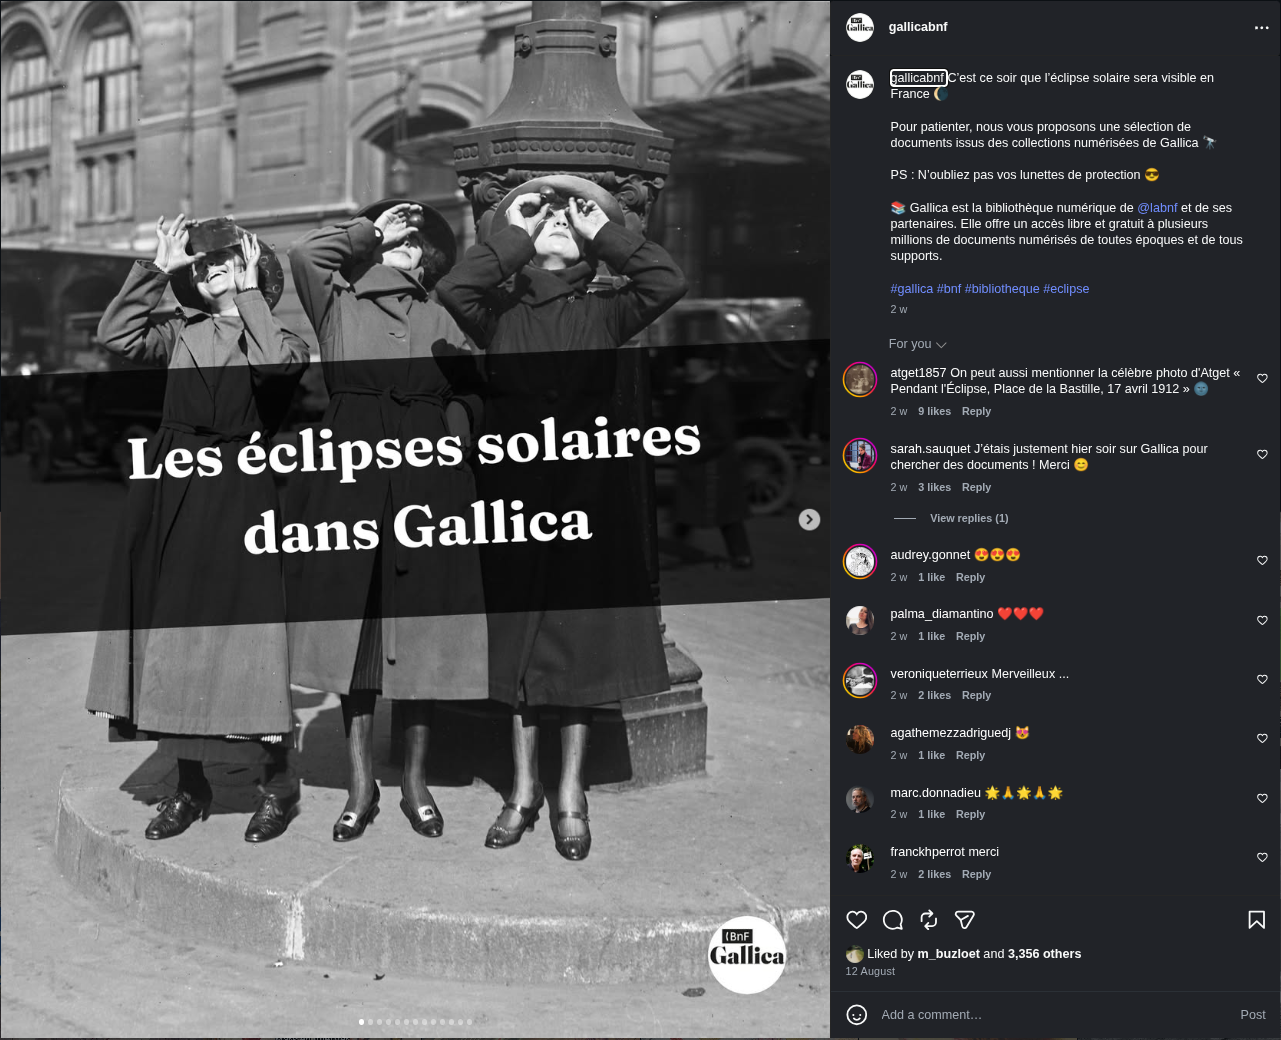
\includegraphics[width=0.24\textwidth]{./illustrations/insta_gallica.png}\hfill
	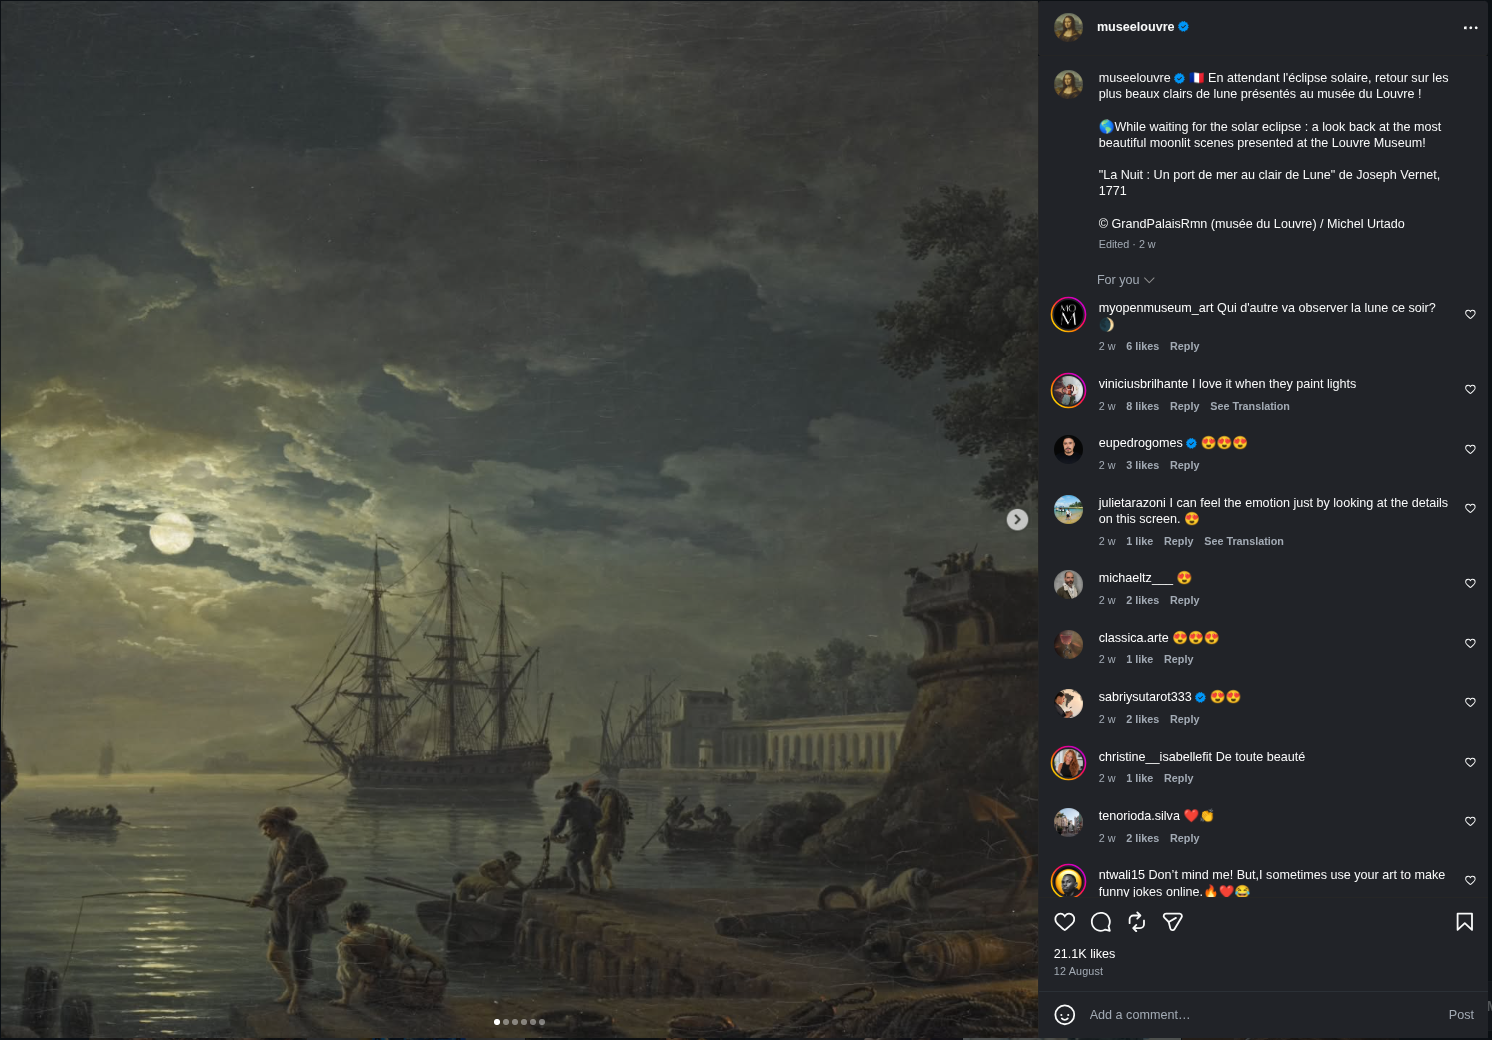
\includegraphics[width=0.24\textwidth]{./illustrations/insta_louvre.png}\hfill
	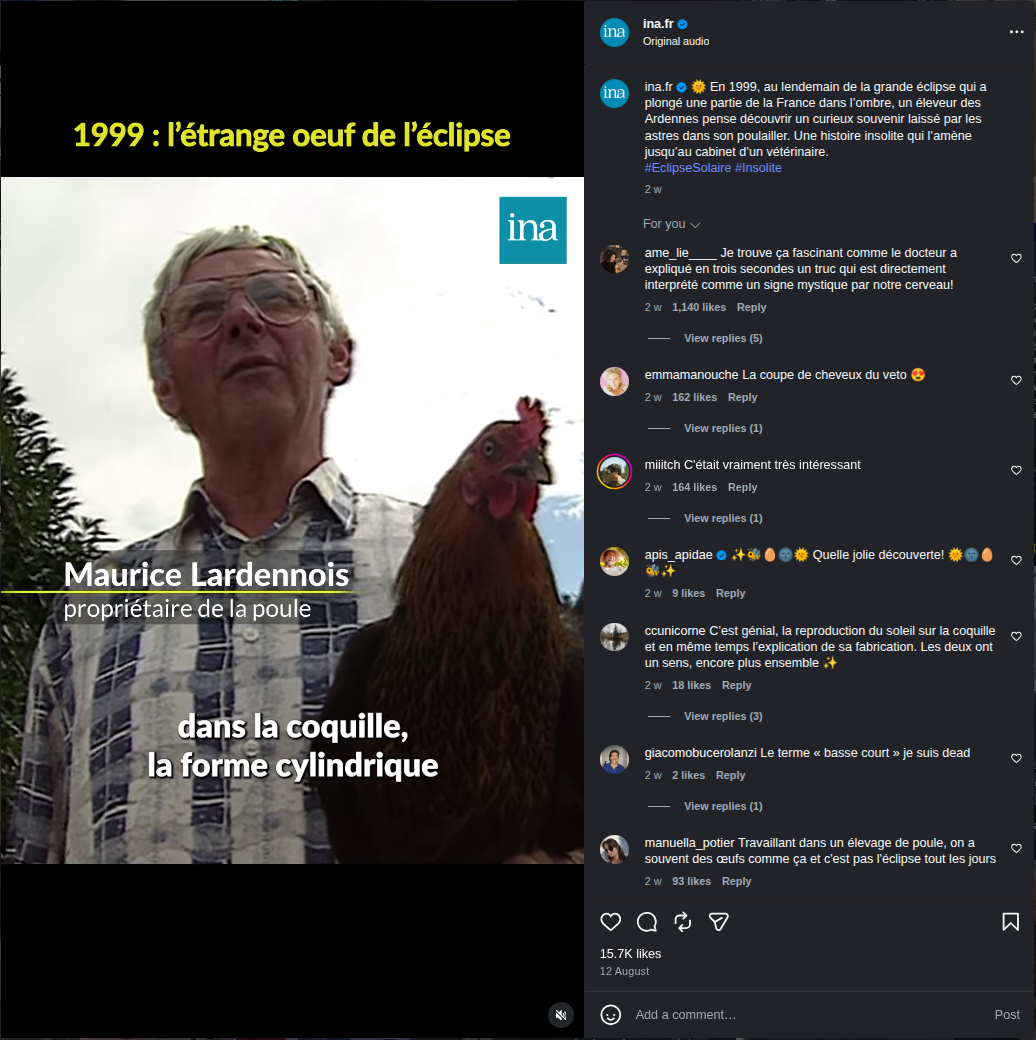
\includegraphics[width=0.24\textwidth]{illustrations/insta_ina.png}
	\caption{Capture d'écran d'une publication du compte officiel des institutions sur instagram le jour de l'éclipse du 12 août 2026 - De gauche à droite : Archives Nationales, Gallica, Louvre, INA}
	\label{fig:insta}
\end{figure}

C'est donc en partie grâce aux réseaux sociaux que le grand public s'est réapproprié ses archives. Au point où aujourd'hui, mêlé à l'innovation de l'intelligence artificielle, ce même grand public, du moins une partie, s'approprie ces documents ou au moins ses codes pour créer de fausses archives. En sa qualité de référent de documents d'archives audiovisuel, l'INA a la responsabilité de sensibiliser les chercheurs au sujet des fausses archives et de l'éthique de la recherche. 

%% Conclusion %%

La conséquence de cette consommation des informations par extraits, via la médiation et l'éditorialisation de l'institution est un public connaissant l'institution, ses collections mais ayant moins de contexte concernant l'archive, sa création, son contexte historique. Cette mode consommation est une véritable rupture, la connaissance ne se transmet plus de la même façon, elle n'est plus recherchée mais découverte. De ce fait, il revient à l'institution et à ses documentalistes de contextualiser et d'apporter le savoir qui accompagne ces documents. Ce public n'est en contact avec les collections que par sa médiation, en conséquent, son accessibilité aux collections ne présente pas d'enjeu important, si ce n'est la responsabilité de l'INA sur la diffusion de fausses archives. Si ce public vient à franchir une salle de lecture, il ne sera plus confronté aux même outils. La confrontation aux bases de données peut être source de frustration en comparaison à la médiation des sites web et réseaux sociaux de l'institution. 
		
		\section{Les chercheurs : évolution de la recherche}
		
		%% Introduction %% 

Sous le terme de \enquote{chercheurs} nous réunissons les personnes exploitant les collections des institutions patrimoniales à des fins de projets de recherche. 

\subsection{L'accessibilité commence par l'acceptation de la pertinence de la recherche}

%% Situer dans le temps %%

Ce sont les premiers à investir les salles de lecture. Le \gls{td} du dépôt légal est principalement à destination de ce public. C'est le premier à investir l'INAthèque et c'est toujours aujourd'hui vers lui que sont destinés ses services ainsi que les compétences des documentalistes. 

Cela dit, si l'étude des sources \enquote{physiques} : manuscrits, cartes, lettres n'ont plus à prouver leur valeur. Les archives audiovisuelles, à la création de l'INAthèque ne disposaient pas de la même légitimité, ce que déplorait Jean-Noël Jeanneney dans \textit{Le Monde} en 1982 : 
\begin{displayquote}
	Il est temps, en effet, que l'évidence s'en impose à tous, bousculant les timidités intellectuelles et les paresses de l'habitude : la télévision a conquis désormais, dans notre vie collective, une importance trop grande pour que l'apport en soit négligé par l'histoire contemporaine, car la connaissance des trois dernières décennies au moins, en serait amputée d'une dimension cardinale\footcite[][10]{zotero-item-735}.
\end{displayquote}
Aujourd'hui, c'est enfin chose faite, grâce aux avancées législatives, technologiques et sociologiques, l'étude de la télévision et de la radio est enfin démocratisée. Certaines institutions de patrimoines télévisés n'ont pas bénéficié de cette ouvertures à l'étude des documents audiovisuels. En Suisse, par exemple, le dialogue entre les acteurs institutionnels et les historiens n'amènent pas à des solutions durables, d'autant plus que le pays n'a pas été avantagé par sa politique fédéraliste, résistant à la centralisation dont les archives audiovisuelles ont bénéficié en France\footcite[][27]{pradervand2013}. Au Brésil, malgré un dépôt légal, l'absence des documents audiovisuels dans les dispositifs légaux de conservation est l'issue d'un manque de considération de la part des politiques ainsi qu'une absence de reconnaissance de la télévision comme un moyen d'expression culturelle\footcite[][58]{Maria2013}. Face au manque d'engouement pour ces collections, ces pays ne bénéficient ni de collections de diffusions télévisées aussi fournie que celles dont nous disposons avec l'INA et encore moins d'un accès facilité à ces collections. Mais à l'INA, de la même manière que l'étude des documents audiovisuels et en général de la télévision et de la radio ont évolué avec le temps, les chercheurs ont fait de même.

\subsection{Le service de l'INAthèque}

%% Services %%

De tous temps, l'INAthèque et ses documentalistes étaient au service des chercheurs et de leurs usages. Ils ont a leur disposition un outil de consultation des collections nommé \enquote{\gls{hy}} grâce auquel ils peuvent rechercher et consulter les notices. En complément de cet outil, les utilisateurs disposent d'autres outils et services. Cela commence par les connaissances dispensées par les documentalistes qui accompagnent les publics de l'INAthèque à l'utilisation de la base de données, à la compréhension et l'exploitation de ses données. S'ajoute à cela des billets de blog décrivant des fonds récemment traités sur le site \enquote{Hypothèse}\footcite[]{2026} auquel les chercheurs peuvent faire appel pour aiguiller leurs recherches. 

Les chercheurs sont les publics externes à l'INA les plus touchés par ces problématiques de \gls{td} et ils sont demandeurs de discussion traitant de ce sujet. C'est d'autant plus bénéfique qu'étant la cible du \gls{td} du dépôt légal, la réflexion qu'ils peuvent apporter est essentielle. Chez les chercheurs, la tendance est à la collaboration et aux échanges, notamment sur la façon qu'ils ont de chercher les documents et en conséquent sur le \gls{td}. 

C'est également une composante que l'on retrouve avec le Lab, crée en 2022. Précédé par des \enquote{ateliers de recherche méthodologique sur le dépôt légal du web}\footcite[][200]{bermès2024}, des ateliers accompagnant les chercheurs aux archives du web en ligne\footcite[]{webcorpora2017}. Le lab est présenté par l'INA comme un \enquote{incubateur de projets}\footcite{zotero-item-700}. Copiloté par la direction des patrimoines et la direction Data \& Technologies, il est composé d'ingénieurs de la recherche et est recentré sur les données. Il propose le même accompagnement de compréhension et d'analyse des documents de la base de données que les documentalistes en salle de lecture mais il se concentre plus particulièrement sur de plus larges jeux de données en accord avec le sujet de recherche des chercheurs accompagnés. Ils élaborent avec eux leur corpus d'étude, les accompagne sur leur pratique des humanités numériques à partir de données audiovisuelles et sur l'utilisation des outils de l'INA. Cet structure fut crée suite aux demandes des chercheurs de plus en plus récurrentes à réaliser des études quantitatives et qualitatives sur des corpus de données très larges, avec l'assistance d'outils de traitement automatique du langage par exemple\renvoientretien{\AH}{les outils et bases de données de l'INA sur les profils de recherche}{ann:transcriptions}

Loin d'être une initiative propre à l'INA, les \enquote{labs} sont des structures mises en place par différentes institutions patrimoniales afin de former le public à ces nouvelles collections entièrement ou majoritairement numériques et aux outils, méthodologies et corpus qui en découlent\footcite[][196]{bermès2024}. Différentes bibliothèques nationales ont suivi ce mouvement au Royaume-Uni (British Library Labs), aux Pays-Bas (KB Lab), aux Etats-Unis (LC Labs)\footcite[197]{bermès2024} et enfin la BNF avec le BNF DataLab\footcite[][199]{bermès2024}. Toutes ces évolutions du \gls{td} ne nécessitent pas seulement une adaptation des bases de données et des outils de consultation mais également une adaptation des services proposés aux chercheurs afin de garantir leur accessibilité aux collections. D'autant plus que leurs recherches, elles aussi évoluent.

%% Outils %%

Concernant les outils à leur disposition, ils se divisent en outils \enquote{experts} et les outils \enquote{autonomes}. Les outils experts comprennent l'outil de consultation \enquote{\gls{hy}}, permettant de faire des paniers de documents audiovisuels consultables dans \enquote{Mediascope}, qui permet de les segmenter et de les annoter ainsi que dans \enquote{Médiacorpus}, qui comme son nom l'indique permet de créer des corpus. Ces outils sont utilisés à l'INAthèque de la BNF ainsi que dans les six délégations de l'INA situées à Rennes, Toulouse, Strasbourg, Lyon, Marseille et Lille. Ils nécessitent l'accompagnement d'un.e documentaliste, au contraire des outils autonomes, présents dans une cinquantaine de lieux partenaires comme des bibliothèques, cinémathèques ou des archives départementales. Les chercheurs de ces lieux partenaires peuvent accéder au fonds du dépôt légal par une interface nommée \enquote{WebMedia} et \enquote{Opsismédia}, sur lesquels ils peuvent visualiser ces documents. Ces outils ont été construits pour répondre aux besoins des chercheurs mais ils sont aujourd'hui vieillissants, fonctionnant sur des OS peu utilisés et manquant de fonctionnalités pour répondre à de nouveaux besoins tel que la possibilité de créer un compte personnel pour créer et stocker des corpus, à partir desquels ils pourraient créer des datavisualisations. L'INA se place cela dit dans la continuité de son adaptation permanente aux nouveaux besoins de ses utilisateurs et a en développement un nouvel outil pour répondre à ces nouveaux besoins nommé \enquote{Skopus}.\footnote{(Ces outils ont été présenté par Arthur Hénaff lors de son entretien, voir sa partie sur les outils et bases de données de l'INA~\ref{ann:transcriptions},\nameref{ann:transcriptions}), p.~\pageref{ann:transcriptions}.}. 

\subsection{Habitudes de consultation des collections}

Ainsi, nous pouvons diviser les chercheurs de l'INAthèque en deux catégories : les chercheurs du Lab qui sont des utilisateurs réguliers des services de l'INAthèque et les chercheurs plus ponctuels, venant pour des recherches personnelles ou accompagnés ou sur la demande de leur professeur durant leur cursus d'études supérieures. Ils effectuent des recherches sur un sujet restreint, parfois donné par leur professeur et utilisent les outils expert avec l'aide des documentalistes. À ces étudiants, les documentalistes ne leur inculque que ce dont ils ont besoin pour effectuer leur recherche. Selon la période, le thème ou le sujet qu'ils souhaitent étudier, ils leur conseillent d'utiliser plutôt les champs titre, mots-clé, résumé ou même d'utiliser du tout-texte, donc de rechercher dans tous les champs, au risque de générer beaucoup de bruit. Leur sujet de recherche peut également avoir pour objectif de créer des statistiques, ils peuvent dans cet objectif rechercher des informations de dates, de temps et d'heure de diffusion. Dans ce même objectif de réalisation de statistiques, ces chercheurs sont très demandeurs de transcription des émissions afin de réaliser des statistiques sur la fréquence de l'utilisation d'un mot. Mais peu importe leur utilisation des collections, la médiation que leur fournie les documentalistes est indispensable à l'utilisation des outils de l'INAthèque. 

%% Conclusion %% 

La première chose que nous pouvons noter est que bien que le profil des \enquote{chercheurs} est très courant dans les institutions patrimoniales, les chercheurs fréquentant l'INAthèque ont bénéficié de politiques favorables à la conservation des diffusions audiovisuelles. En conséquence, l'INA fait posture de précurseur dans tous les outils qu'elle met en place pour la communication de fonds audiovisuels étant donné que la richesse des collections de cette institution la placent en exception dans le monde patrimonial à l'échelle mondiale. Cela dit, les chercheurs sont les publics les plus touchés par ces enjeux d'accessibilité aux collections des institutions patrimoniales. Ils sont pleinement dépendant des outils crées par les institutions patrimoniales et plus particulièrement de l'expertise des documentalistes. Ces derniers leurs fournissent les clefs pour comprendre et exploiter les outils et collections de l'institution. 
		
		\section{L'expertise du documentaliste : apprendre, transmettre, s'adapter}
		
		%% Introduction %%

Nous allons dès à présent appuyer sur le métier de documentaliste et sa relation avec les collections et bases de données ainsi que sur l'importance de leur expertise dans la médiation des collections.

%% Situer dans le temps %%

Il va de soi que les premières personnes concernées par les bases de données, les données de descriptions et le \gls{td} appliqués sont les personnes travaillant au sein des institutions patrimoniales. C'est en partie à travers leurs besoins, leur expertise et leurs recommandations que les politiques documentaires sont élaborées. Pour autant, l’accessibilité aux collections reste un enjeu de tous les jours. 

\subsection{Connaissances de outils de consultation et de production des bases de données}

%% Habitudes, données de description préférées %%

Au fur et à mesure des années, des changements dans les bases de données et de la mise en place de nouveaux outils, les professionnels de l'INA ont construits leurs habitudes sur ces changements. Quand les archives professionnelles et le dépôt légal étaient séparés, les outils de consultation des bases de données l'étaient aussi. Une fois les services réunis, les documentalistes conservent majoritairement leurs habitudes. La documentaliste que nous avons interrogé, anciennement au dépôt légal, continue majoritairement à utiliser \gls{hy}, l'outil de consultation du dépôt légal mais dans le cas de reprise d'antériorité, elle doit utiliser \gls{to}, l'outil de consultation et de production des archives professionnelles, duquel dépendent les reprises d'antériorité. Ces professionnels sélectionnent donc leurs outils en fonction de leurs habitudes mais également en fonction des missions. Malgré la réunification des services des archives professionnelles et du dépôt légal, les deux outils ont des usages différents. La transition vers un nouvel outil peut être difficile, comme l'est actuellement la transition vers l'outil de consultation Notilus\renvoientretien{\DA}{les bases de données de l'INA}. Ce dernier n'est pour le moment qu'à usage interne, il a été mis en place dans des contextes différents d'\gls{hy} et \gls{to}. Il contient toutes les transcriptions réalisées par IA dans lesquelles il est possible de faire des recherches tout-texte ainsi qu'une recherche sémantique, ces deux fonctionnalités pouvant compenser le manque d'informations des données de description comme c'est le cas dans les fonds de l'ORTF\renvoientretien{\PL}{les bases de données de l'INA}.

Une part du métier reste l'adaptabilité. Ces experts doivent pouvoir répondre à toutes les questions des chercheurs, quel que soit leur sujet. De plus, ayant connaissance des collections de l'INA, ils doivent pouvoir faire appel à chaque outils à leur disposition. C'est pourquoi ils ont l'habitude d'utiliser ces trois outils de consultations mais certains font également appel aux fiches papier ou aux archives physiques. Quand une information dans la base de données est incohérente, la réponse peut se trouver dans un programme TV par exemple\renvoientretien{\PL}{l'expertise du documentaliste}. 

\subsection{L'expertise du documentaliste}

Si les chercheurs ont un sujet privilégié qu'ils vont explorer avec l'aide des documentalistes. Ces dernièr.es doivent avoir une connaissance parfaite des fonds, c'est \enquote{l'expertise du documentaliste}. Ces professionnels ont une connaissance poussée sur le fonctionnement des bases de données, sur les différentes politiques documentaires, sur la construction et l'acquisition des collections. Cela ne concerne évidemment pas que l'INA, les documentalistes acquièrent une expertise dans le domaine dans lequel ils exercent. C'est pourquoi, dans le cadre de commandes, les documentalistes de l'INA peuvent faire appel à des documentalistes en dehors de l'INA, dans le cas où les documents nécessaires ne sont pas dans leurs fonds mais dans les fonds d'une autre institution.

Pourtant, c'est aujourd'hui une connaissance qui est en péril. Il y a plus de 30 ans, le dépôt légal des documents audiovisuels chamboulait le fonctionnement de l'INA, à cette occasion, plusieurs documentalistes ont été engagé.es pour accompagner ce nouveau flux entrant de documents. Ce qui signifie qu'actuellement, les documentalistes ayant vu naître et grandir ce dépôt légal approchent de la retraite ou y sont déjà. Le \gls{td} n'ayant pas ou peu été documenté, il est plus que jamais essentiel qu'ils.elles transmettent leurs connaissances comme leurs prédécesseuses l'ont fait. C'est une démarche déjà entamée pour leur connaissance des fonds. Dans le cas où ces professionnelles investissent beaucoup de temps sur un fond, sur une typologie ou sur un sujet, elles en deviennent des expertes et sont en capacité de transmettre leurs connaissances à travers les corpus qu'elles construisent. Nous retrouvons ces corpus dans l'outil de consultation et de production \enquote{\gls{to}} ou sur les différentes plateformes de médiation de l'INA\renvoientretien{\PL}{l'expertise du documentaliste}. 

Malheureusement, leurs connaissances sur le \gls{td} ne sont pas aussi bien documentées, ce qui est un point important à mettre en avant dans la construction de notre outil de cartographie du \gls{td}. De cette façon, l'accessibilité aux bases de données de l'INA par les documentalistes sont soumises aux mêmes enjeux que les chercheurs à la différence qu'ils possèdent toutes les clefs pour comprendre et utiliser les bases de données de l'institut. 
		
		\section{La spécificité de l'INA : les professionnels de l'audiovisuel}
		
		%% Situer dans le temps %%

Pour terminer sur ces publics des institutions patrimoniales, nous allons nous attarder sur un public assez exclusif à l'INA : les professionnels de l’audiovisuel et de façon plus général toutes les institutions professionnelles ayant recours aux images conservées ou produites par l'INA. C'est le seul public externe à l'institution que l'on peut situer dès la création de l'INA et même précédant sa création, à la cinémathèque. Pourtant, tous comme les autres publics que nous venons de présenter, il a connu une évolution importante depuis les débuts de la conservation des documents audiovisuels télévisés. A l'origine, les commandes aux cinémathécaires et aux documentalistes étaient destinées aux chaînes télévisées et leur programmes, souvent des journaux télévisés. Par exemple, notre documentalistes interrogée répondait aux commandes de TF1 avant la mise en place du dépôt légal à l'INA\footnote{(Voir entretien d'une documentaliste sur la présentation de son parcours à l'INA ~\ref{ann:transcriptions},\nameref{ann:transcriptions}), p.~\pageref{ann:transcriptions}.}. Aujourd'hui, c'est le service \enquote{Clients et partenaires} qui répond à ces commandes\footnote{(Voir organigramme de la direction des patrimoines ~\ref{ann:org},\nameref{ann:org}), p.~\pageref{ann:org}.}. Seulement, les commandes auxquelles ce service répond s'étend désormais bien au delà des chaînes de télévisions, bien qu'elles sont inclus dans leurs interlocuteurs parmi lesquels on compte les commandes pour des journaux télévisés ou pour des documentaires. A cela s'ajoute les productions de l'INA tel qu'\enquote{ADN}, \enquote{Rambob'INA}, \enquote{Témoins d'Actu}, des plateformes de streaming comme Netflix et des institutions culturelles, incluant toutes les commandes à destination d'expositions\footnote{(Voir entretien de Pascal Lebeurier sur la présentation de son parcours ~\ref{ann:transcriptions},\nameref{ann:transcriptions}), p.~\pageref{ann:transcriptions}.}. 

%% Outils %%

Ces professionnels ont à leur disposition l'outil inamediapro\footcite[]{zotero-item-696}. Grâce auquel ils peuvent explorer les documents de la base de données des archives professionnelles, visionner un extrait en basse qualité, le segmenter, l'annoter, le partager et passer commande. Si l'INA possède bel et bien tous les droits pour la commercialisation de cet extrait, ils recevront leurs extraits en meilleure qualité ou seront informés des frais à envisager pour son exploitation. De la même façon qu'ina.fr, une médiation ciblée est proposée par personnalité, thème ou par évènement. 

\begin{figure}[H]
	\centering
	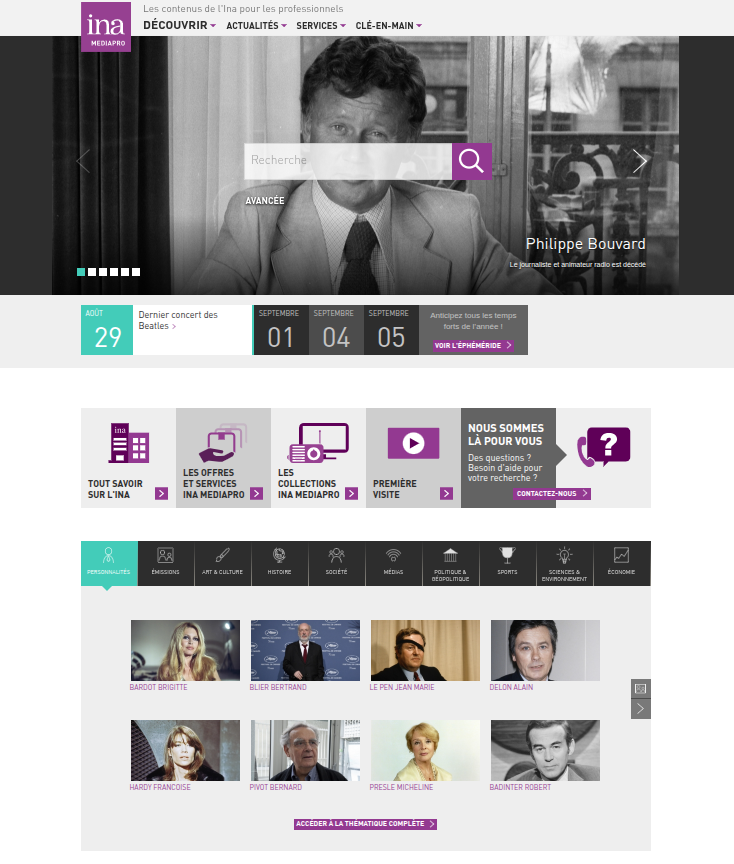
\includegraphics[width=1\linewidth]{./illustrations/inamediapro.png}
	\caption{Capture d'écran du site inamediapro.fr}
	\label{fig:inamediapro}
\end{figure}

Pourtant, l'aide d'un professionnel de l'INA est souvent requis afin de faire aboutir leurs demandes. Pascal Lebeurier, cadre documentaliste au service \enquote{Clients et partenaire} statue que souvent, ces professionnels préfèrent faire appel à des documentalistes pour leur recherche, considérant que ce n'est pas leur métier et qu'ils ne le feront pas mieux qu'un documentaliste ou par peur de manquer des images intéressantes par manque de compétence et de connaissance des fonds. Ce service payant, fait partie de cet éventail de compétences que les documentalistes mettent au service des utilisateurs externes à l'INA. Dans cette situation, l'outil inamediapro ne sert qu'à visualiser les extraits suggérés par le documentaliste s'occupant de cette demande.

%% Habitudes, données de description préférées %%

Les documents recherchés varient évidemment beaucoup de l'interlocuteur : cela peut être une recherche sur une personnalité. Dans ce cas, les champs mis à contribution sont le génériques si c'est une personnalité susceptible d'y apparaître. Selon le contexte, d'autres champs peuvent être mis à contribution. Pour \enquote{Nikos Aliagas} les mots-clés tel que la \enquote{Grèce} ou des thèmes comme la \enquote{Dictature des colonels} ont été mobilisés. Des sujets plus conceptuels vont demander de faire appel à plus de réflexion et de recherche, notamment sur l'indexation. Pour une recherche sur la saleté dans Paris, il est plus judicieux de s'intéresser à une campagne de propreté dans Paris, qui évoquera sans doute la saleté\footnote{(Voir entretien de Pascal Lebeurier sur les profils de recherche ~\ref{ann:transcriptions},\nameref{ann:transcriptions}), p.~\pageref{ann:transcriptions}.}. 

%% Conclusion %% 

Dans cette typologie de public et d'utilisateurs des collections de l'INA, l'expertise du documentalistes est tout aussi importante, voire plus que pour les chercheurs. Même si ils ont à leur disposition un outil de consultation et de sélection de documents à commander, certains préfèrent directement faire appel à des documentalistes afin de ne pas souffrir de leur manque de connaissance sur les fonds de l'institution. Une fois de plus, l'accès aux collections de l'INA dans leur entièreté n'est pas autonome. 
	
	\chapter{Impact de l'hétérogénérité des données sur les pratiques des publics des institutions patrimoniales}
		
		\section{Manque de connaissance des périmètres de l'INA}
		
		%% Introduction au problème %%

Le principal frein à l'accessibilité de l'ensemble des collections de l'INA est l'absence de compréhension par ces publics, de l'organisation des dites collections. En ignorant comment a été réalisé la collecte, la conservation, la description et l'indexation de ces documents, il est difficile de savoir comment effectuer sa recherche. Dans l'ensemble, les utilisateurs des bases de données de l'INA, avant la médiation des documentalistes, n'ont pas vraiment conscience de ce que conserve l'INA. Le périmètre de leurs fonds sont flou pour un public externe. Ils vont par exemple chercher à l'INA des images de la première guerre mondiale quand ces images sont conservées à l'ECPAD (Établissement de communication et de production audiovisuelle de la Défense). En conséquence, les utilisateurs ont encore moins conscience des politiques documentaire. Il est difficile de savoir dans quel champs chercher. Pour une émission diffusée avant 1975, il vaut mieux ne pas utiliser de mots clés mais d'un autre côté, en effectuant une recherche plein-texte, les résultats sont très bruyants. De plus, quand on ne connais pas la base de données comme les connaissent les documentalistes, il est aisé de faire un contre-sens, de faire une recherche, d'avoir un certain nombre de résultats et s'y tenir, sans savoir qu'en utilisant un autre champs ou un autre mots-clé, les résultats auraient été bien plus nombreux\footnote{(Voir entretien d'une documentaliste de l'INA sur l'expertise du documentaliste~\ref{ann:transcriptions},\nameref{ann:transcriptions}), p.~\pageref{ann:transcriptions}.}. 

%% Application à chaque public %%

C'est alors que les questions se dirigent vers les documentalistes, détenteurs de ce savoir, soit pour se décharger de la recherche documentaire comme le font les professionnels de l’audiovisuel dont la recherche n'est pas le domaine et qui ne souhaitent pas en faire souffrir leur créations, soit pour acquérir les connaissances nécessaires pour effectuer leurs recherches. L'expertise des documentalistes est d'une grande valeurs. C'est pourquoi une de leurs missions consiste à le concrétiser en outils facilitant la compréhension de ces collections comme le sont la création de corpus et l'écriture de billet de blog pour le blog \enquote{Hypothèse}. Malgré tout, les documentalistes ne sont pas omniscients, leur connaissance a des limites. Elle ne peut pas s'étendre aux nombreux cas particuliers qu'ils n'ont jamais étudiés ou à la connaissance d'indexations utilisée avant qu'ils ne prennent leur poste. 

Ce premier frein à la recherche dans les bases de données des collections de l'INAthèque est également implicite dans les autres problèmes que nous allons soulever. Chaque frein à la pleine accessibilité des collections existent en partie parce que les utilisateurs n'en ont pas forcément conscience. 
		
		\section{Un problème de qualité}
		
		%% Introduction du problème %%

Nous ne pouvons pas non plus ignorer que ces institutions patrimoniales conservent un nombre conséquent de données, renseignées pour la plupart manuellement. Il est donc hautement probable que des erreurs persistent parmi les données, parfois à cause d'un manque de référentiels et d'autres simplement à cause de l'erreur humaine. Autant sur certains champs comme le titre qu'au sein même de l'indexation, notamment de noms propres. Au cours de l'exploration des données d'une des bases de données du dépôt légal, nous avons ainsi relevé sans difficulté 3 émissions dont il existait deux entités différentes : \enquote{Arte Journal} et \enquote{ARTE journal}, \enquote{13h15 le dimanche} et \enquote{13h15 le dimanche.}, \enquote{Mardi cinéma, le dimanche aussi !} et \enquote{Mardi cinéma, le dimanche aussi. [Le mag].}. Ces erreurs peuvent empêcher certaines fiches de ressortir lors d'une recherche. La réalisation de statistiques peut également en être entachée. Ce sont les mêmes conséquences pour les indexations de noms propres. Pascal Lebeurier évoque dans son entretien les longues recherches nécessaires pour retrouver le nom de footballers mal indexés dans fiches anciennes\footnote{(Voir entretien de Pascal Lebeurier sur l'expertise du documentaliste ~\ref{ann:transcriptions},\nameref{ann:transcriptions}), p.~\pageref{ann:transcriptions}.}. Sans que d'erreurs manifestes ne soient commises les fiches peuvent également varier. Si deux notices de deux épisodes d'un même programme sont réalisés par deux personnes différentes, l'indexation appliquée peut varier. Nous ne pouvons pas parler \enquote{d'erreur} mais cela entraîne tout de même une variation dans les résultats selon la recherche qui est effectuée et tous documents voulus ne ressortirons pas. 
		
		\section{Nouveau mode de consommation des informations}
		
		\subsection{Nouvelles disciplines d'étude}

%% Introduction au problèmes %%

Pour finir, les profils des chercheurs ont changé au contact de la numérisation, ils n'ont pas les mêmes besoins qu'avant qu'elle n'intègre les salles de lectures. Le premier indicateur en est l'intérêt que portent les chercheurs aux archives audiovisuelles, qui comme nous l'avons vu, n'a pas toujours bénéficié de la même légitimité que l'étude des manuscrits ou des archives. Ce constat s'applique également à une institution patrimoniale plus ancienne comme la BNF, qui au cours d'une études sur les usages documentaire des chercheurs détermine que l'intérêt de leurs lecteurs se sont de plus en plus portés vers de nouvelles disciplines\footcite{pardé2015}. Si l'on considère que l'indexation est établit en fonction des usages et besoins de ses utilisateurs au moment où elles sont utilisées, cela crée aujourd'hui un décalage entre l'indexation utilisée dans les notices documentaires et ce que recherchent effectivement les usagers. 

%% Application à chaque public %%

Il devient alors nécessaire de comprendre quelle indexation a été utilisée et de développer les pratiques nécessaires pour contourner ces problématiques. Sans cela, une recherche par mot-clé n’aboutis pas au résultat espéré, ils sont amoindri car le vocabulaire utilisé est obsolète, pensons par exemple au termes de \enquote{féminicide}, \enquote{réchauffement climatique} qui ne trouveront pas leur place dans des notices anciennes. Impossible dans ce cas, en faisant uniquement appel l'indexation d'analyser le traitement de l'actualité sur ces sujets dans les journaux télévisés des années 80. La clef de ce décalage est bien souvent l'expertise documentalistes, qui dotés de leurs expertises sur les collections ont connaissance de ce décalage et peuvent offrir des solutions ou même éventuellement mettre en place une médiation et construire des corpus en fonction de l'actualité comme c'est réalisé sur le site ina.fr mais également dans les émissions produites par l'INA, étudiant des sujets d'actualités à la lumières de documents audiovisuels d'archives. 

\subsection{De nouveaux publics}

Les publics touchés par ces collections sont également bouleversés, le grand public est de plus en plus touché par ces collections mais il ne les consomme pas en salle de lecture comme le font les chercheurs. La consommation des collections s'est déplacée en ligne. En conséquent les habitudes de consommation s'adaptent aux formats conçus à ce grand public des sites web où la découverte fortuite de nouvelles images est aisée à l'époque des algorithmes personnalisés. Au sein de la salle de lecture, cette aspect de découverte se perd. Difficile d'arriver en salle de lecture sans savoir ce que l'on recherche, les outils de consultation ne sont conçus que pour répondre à une chaîne de caractères précise, pas à une vague envie de découvrir son patrimoine audiovisuel. Là encore, il n'y a que les documentalistes pour venir en aide à ces nouveaux publics s'aventurant en salle de lecture. 
		
\chapter*{Conclusion de la partie 1}

De l'analyse de ces différents profils d'utilisateurs des collections de l'INA, une conclusion revient sans manquer, la bonne accessibilité aux collections repose en grande partie sur l'expertise des documentalistes, qui est pourtant en péril aujourd'hui. Le travail des documentalistes reste extrêmement important, que cela soit lors du traitement documentaire ou lors de la médiation de connaissances. Actuellement, si il n'y a aucune médiation des documentalistes, à l'INAthèque ou par la création de corpus, la compréhension de la base de données est compromise.

Il est donc au centre de nos préoccupations, afin de faciliter l'accessibilité aux collections de donner aux utilisateurs de nouvelles clefs de compréhension des bases de données de l'INA. Notre projet de cartographie doit donc se concentrer sur le partage des connaissances et la cartographie visuelle du traitement documentaire afin de donner toutes les clefs aux utilisateurs pour comprendre ces collections. Mais pour le mettre en place, nous devons déjà identifier quels paramètres génèrent ces difficultés à accéder à l'ensemble des collections de l'INA. Tout comme il est important de prend en compte les solutions déjà mises en place pour faciliter l'accessibilité aux collections. 
		
	
\part{De quel contexte sont issues ces données hétérogènes ?}

Afin de trouver des solutions pour améliorer l'accessibilité aux collections d'institutions patrimoniales, il est donc nécessaire de comprendre pourquoi et comment l'évolution des pratiques documentaires est arrivée à cette situation inconfortable pour les utilisateurs. Dans cet objectif, nous allons décrire les principaux facteurs d'évolution des politiques documentaires dans les institutions patrimoniales et quelles conséquences cela a eu dans la documentation des collections. Pour cela, nous avons séparés ces facteurs en deux. 

%% Chapitre 3 %%

Les facteurs d'ordre sociaux dans lesquels nous décrirons l'évolution du contexte légal de la conservation et de la communication des documents audiovisuels et plus particulièrement le rôle que tient l'INA dans cette mise en place d'un cadre légal. En lien avec ce cadre légal, nous nous arrêterons sur le changement de statut et d'usage des documents conservés et la réflexion que cela entraîna sur le traitement documentaire. Puis nous développerons l'impact des changements institutionnels entraînés par le dépôt légal sur la qualité des données et nous conclurons avec les contraintes motivées par le contexte économique. 

%% Chapitre 4 %%

Dans un second temps, nous développerons l'impact des nouvelles technologies sur le traitement documentaire en retraçant l'évolution de la discipline de la documentation de ses débuts à son informatisation puis nous comparerons cette évolution à l'accès que proposent les outils de consultation et de production des bases de données de l'INA. Puis, nous établirons un état du traitement documentaire contemporain en développant la notion de \enquote{Big Data} et en analysant l'impact de l'intelligence artificielle sur la documentation des institutions patrimoniales. 

\chapter{Un contexte social en mouvement}

	\section{Mise en place d'un cadre légal}
	
	%% Introduction %%

Michel Melot établit le patrimoine comme une composante indispensable d'une communauté\footcite[]{melot2004}. En cela, un patrimoine ne nécessite, pour exister, que d'être désigné par une communauté comme représentatif de leur groupe. Or, dans ce mémoire, nous nous intéressons aux institutions patrimoniales, c'est-à-dire des organismes chargés de leur collecte, de leur conservation et de leur diffusion. Dans ce sens, la mise en place de ces institutions répond au besoin de ces communautés de désigner un gardien de leur patrimoine. Ces institutions peuvent être d'ordre privé comme l'est la \enquote{Société d’histoire et d’archéologie du Sedanais} qui prône la \enquote{Sauvegarde et mise en valeur du patrimoine historique et archéologique du pays sedanais}\footcite[]{sedan} ou encore comme le \enquote{Centre archives LGBTQI+} à Paris par lequel cette association LGBT+ exprime le besoin de \enquote{créer, collecter, classer, conserver et communiquer les archives LGBTQI+ à tous les publics}\footcite{lgbt}. Cela dit, nous resserrerons notre propos sur les institutions patrimoniales publiques, à laquelle appartient l'INA. Cette différenciation a une importance car si les institutions privées exercent librement leurs missions sans contrainte autre que celles qu'elles s'imposent, les institutions publiques sont sous l'autorité d'un État qui les désigne comme responsable d'un patrimoine national. En conséquent de quoi, leurs missions sont encadrées par des textes de loi désignant le patrimoine dont elles ont la responsabilité ainsi que le public auquel la communication du patrimoine conservé est destiné. C'est pourquoi il nous est essentiel de débuter cette analyse du contexte d'évolution du traitement documentaires des institutions patrimoniales en étudiant les lois qui les définissent et nous donnent une trace de leurs origines. C'est pour les respecter que les politiques documentaires appliquées répondent en premier aux prérogatives définit par ces textes de loi. 

\subsection{Avant l'INA, les cinémathécaires}

%% Post-INA %%

En 1949, dans l’ordonnance qui définit le statut de la RTF\footcite[]{zotero-item-335}, nous ne pouvons qu’interpréter dans ces mots une des futures missions de l’INA : 
\begin{displayquote}
	la Radiodiffusion-Télévision française [\dots] a seule qualité, dans les territoires de le République pour [\dots] radiodiffuser ses programmes et ou les mettre à la disposition d’autres organismes radiodiffuseur.
\end{displayquote}
En 1964, l’ORTF poursuit cette même mission\footcite[]{zotero-item-645} et 10 ans plus tard, quand Marceau Long présente le projet d’éclatement de l’ORTF, ces missions ont totalement disparues et l’INA ne figure pas encore dans les établissements publics résultant de la dissolution\footcite[][118]{cohen2021}. Ce n’est que dans la loi statuant de l’éclatement de l’ORTF, le 07 août 1974, que ses principales missions apparaissent enfin clairement et officiellement :  
\begin{displayquote}
	Il est créé un institut de l’audiovisuel chargé notamment de la conservation des archives, des recherches de création audiovisuelle et de la formation professionnelle.\footcite[]{zotero-item-331}
\end{displayquote}
Pourtant, dans cet intervalle, la mission de conservation et de communication des diffusions audiovisuelles n'est pas à l'abandon, elle est portée par celles que l’on appelait alors les « cinémathécaires ». Malgré le manque de reconnaissance social, politique et institutionnel de leurs activités\footcite[][182]{tible2023} elles posent les bases de que nous appelons aujourd’hui le traitement documentaire. Elles réalisent les « prises d’antenne », les indexations et recherchent les documents commandés par les chaînes de télévision de l'ORTF. Les informations sont sur fiches papier et sont indexées par thème ou par personnalité. On crée autant de fiches qu’il y a de thèmes indexés et elles sont rangées dans des meubles classeurs dédiés. Ces fiches doivent permettre à ces mêmes documentalistes de retrouver aisément les émissions demandées par les chaînes de télévision. En effet, la mission de communication est restreinte par la fragilité des supports audiovisuels. Il n'est pas envisageable de visionner plusieurs documents à chaque commande, autant du point de vue de la conservation que du temps consacrer à la recherche de contenu.

\subsection{Premières années d'existence : la commercialisation des images}
%% INA avant le dépôt légal %%

Ce sont donc sur ces bases que repose le traitement documentaire effectué à la création de l’INA. Cela dit, contrairement à ce que cela sous-entend quand on évoque la « conservation des archives », ces fiches ne sont pas empreintes de la volonté de patrimonialisation. L’INA vend ses documents et ses notices sont élaborées en fonction de ce besoin. Nous n'en sommes pas encore à désigner l'INA comme une \enquote{institution patrimoniale}. Cette vision des archives change progressivement au cours des années 70 et 80. La notion de patrimoine se popularise quand elle est employée par l'UNESCO en 1972 et la conservation des \enquote{images en mouvement} prend son importance avec les recommandations de l'UNESCO pour la sauvegarde et la conservation des \enquote{images en mouvement} le 27 octobre 1980\footcite[]{unesco}. En France c'est la loi dites « Léotard » en 1986\footcite[]{zotero-item-334} qui manifeste ce besoin d'introduire ces documents à la patrimonialisation. Elle ouvre la télédiffusion aux entreprises privées et appuie les missions de conservation et d’exploitation de l’INA :
\begin{displayquote}
	(INA), est chargé, [\dots]] de conserver et exploiter les archives audiovisuelles des sociétés nationales de programme. 
\end{displayquote}
Mais cette exploitation reste limitée aux chaînes de diffusions nationales et publiques, et uniquement à des fins professionnelles. 

\subsection{Le dépôt légal}
%% L'INA et le dépôt légal %%

C’est la loi qui implémente le dépôt légal de la radio et de la télévision, le 20 juin 1992\footcite[]{zotero-item-332} qui va durablement ajouter la patrimonialisation aux missions de l’INA et ouvrir l’exploitation des documents qu’elle conserve à des fins scientifiques\footcite[][23]{varra2023}.  
\begin{displayquote}
	L’institut national de l’audiovisuel est chargé de recueillir et de conserver les documents sonores et audiovisuels radiodiffusés ou télédiffusés, de participer à la diffusion des bibliographies nationales correspondantes et de mettre ces documents à la disposition du public pour consultation.
\end{displayquote}
C'est une étape importante dans l'histoire du traitement documentaire à l'INA. Le traitement de ces documents doit désormais s’adapter à une exploitation commerciale et scientifique. D’autant plus que l’INA ne peut vendre que des programmes sur lesquels elle a les droits, ce qui n’inclue pas tous les documents conservés au titre du dépôt légal. Ces documents constituent une exception au droit d’auteur. L’INA a le droit de les exploiter et de les diffuser uniquement à des fins scientifiques. Cette multiplication des missions donne naissance à une modification importante du fonctionnement de l’INA\footcite[][23]{varra2023}. L'usage des documents que conservent l'INA change radicalement et la description doit s'y adapter. Avec le dépôt légal, il n'est plus seulement question de créer des fiches pour les documents permettant de retrouver des thèmes ou des personnalités. En conséquence, est créé à l’INA une nouvelle direction pour héberger cette nouvelle mission patrimoniale et dès 1995 est ouvert le centre de consultation du dépôt légal à la Bibliothèque François Mitterrand. Cette loi, marquant un changement radical dans le traitement documentaire, est le parfait exemple d'une loi impactant le public cible du traitement documentaire et en conséquent ce qu'il décrit dans le document. Par la suite, le champ du dépôt sera précisé par un décret\footcite[]{zotero-item-330} et continuera de s’étendre à d’autres chaînes et d’autres programmes\footcite[][25]{varra2023}, notamment avec l’arrivée de la TNT, puis des programmes télévisés sur le web\footcite[]{zotero-item-647}. En 2004, le dépôt légal est intégré au code du patrimoine\footcite[]{2004}, qui remplace la loi de 1992.

%% Le dépôt légal dans d'autres institutions %%

Il y a encore quelques années, ces documents audiovisuels étaient uniquement conservés, aux yeux de la loi, dans un objectif de consommation. Avec le dépôt légal, ces documents audiovisuels font l’objet d’une nouvelle injonction à la patrimonialisation. Ils s’inscrivent désormais dans un patrimoine national\footcite[][74]{bermès2024} et les politiques documentaires de l’INA s’en voient questionnées. Là où le public cible était unique, il est désormais multiple et les impératifs métiers concernant le traitement documentaire doivent s’adapter à des prérogatives légales. En effet, il est dans la nature du dépôt légal, dès sa création en 1537, de léguer un discours national aux générations futures. En s'appliquant aux documents audiovisuels télévisés, le dépôt légal l'inscrit dans le patrimoine national français. D’abord destiné aux livres, le dépôt s’étendra au fur et à mesure à plusieurs supports permettant la transmission de la pensée\footcite[][18-19]{saby2013}. Aujourd’hui, les institutions patrimoniales qui sont chargées du dépôt légal aux côtés de l’INA sont le CNC pour l’image animée\footcite[]{zotero-item-673} et la BnF pour les livres périodiques, documents cartographiques, iconographiques ainsi que la musique imprimée et les documents sonores et vidéogrammes\footcite[]{zotero-item-675}. Pourtant, malgré cette injonction légale commune, ces institutions ne proposent pas le même traitement documentaire, elles répondent individuellement aux restrictions qu’imposent leurs supports mais elles s’appuient également sur leur histoire. Toutes ces institutions n’ont ni crée le traitement documentaire, ni attendu le dépôt légal pour établir des méthodes de traitement, comme nous l’avons vu avec les cinémathécaires de l’ORTF. La principale différence réside dans l’héritage dont ils disposent. En 1537, les livres n’étaient pas des supports récents, au contraire des diffusions audiovisuelles, télévisées et radiophoniques. Ces supports n’ont pas hérité de centaines d’années de réflexion sur leur traitement documentaire et leur catalogage. Bien qu'elles puissent s'inspirer des traitements appliqués à d'autres supports. Le dépôt légal n’a pas fait qu’institutionnaliser leur conservation, il a institutionnalisé la réflexion sur leur traitement dans un objectif de communication scientifique et de patrimonialisation. 

Dans ce cadre, nous pouvons questionner le traitement documentaire dans un cadre où le dépôt légal n’a pas institutionnalisé la conservation de ses diffusions télévisées. En Suisse, malgré une loi nommée « dépôt légal », la RTS ne conserve que des émissions\footcite[][11]{griveau2024}, et non l’entièreté du flux, 24 heures sur 24, comme le fait l’INA depuis 2001 grâce à un dispositif de captation numérique par liaisons satellites et fibre optique\footcite[][23]{saby2013}. Le flux télévisuel n’est donc pas conservé. Les émissions de leur fond ont été sélectionnées en fonction de critères documentaires tels que leur réutilisation\footcite[][16]{griveau2024}, conservant une logique commerciale. Actuellement, les fonds de la RTS sont de 680 000 heures\footcite[][13]{griveau2024} contre 28 172 492 heures au titre du dépôt légal le 31 décembre 2025\footcite[]{zotero-item-655} à l'INA. Aux États-Unis la librairie du congrès ne conserve que 3.5 millions d’heures d’enregistrements de toutes origines, y compris la radio\footcite[]{zotero-item-654} et une partie des archives audiovisuelles des « National Archives » manquent encore de description\footnote{(Voir entretien de Pascal Lebeurier sur l'expertise du documentaliste~\ref{ann:transcriptions},\nameref{ann:transcriptions}), p.~\pageref{ann:transcriptions}.}.

%% Conclusion et ouverture à la sous-partie suivante %%

L'exemple de l'INA est une bonne représentation de l'impact que peut avoir le cadre légal sur une institution. À la naissance de la conservation des supports audiovisuels télévisés par les cinémathécaires de l'ORTF, la notion conservation patrimoniale est de moindre importance en comparaison de l'importance portée à la conservation à but commerciale. Les informations que l'on retrouve dans les fiches ont pour objectif de répondre à ces usages. Elles doivent permettre de trouver rapidement des images pour illustrer les émissions. Ce n'est que quand le dépôt légal est appliqué à la télévision que l'institut national de l’audiovisuel est considéré comme un institut véritablement à but patrimonial. Le traitement documentaire est désormais destiné à un nouvel usage scientifique où la rapidité à trouver une information importe moins que de transmettre une description de l'ensemble du flux télévisé afin de répondre à de nouveaux usages, de nouveaux besoins, de nouvelles pratiques, sans toujours savoir ce que ce nouveau public attendra. Ce nouveau service du dépôt légal doit associer les mêmes contraintes de fragilité des supports avec un nouveau public pour lequel la consultation des documents s'inscrit dans leurs pratiques. D'autant plus que cela s'accompagne d'une massification des collections de l'INA et des données les décrivant. Nous décrirons plus en détail cette massification des données et comment ils impactent le traitement documentaire. Mais avant cela, pour appuyer sur l'impact majeur qu'a cette loi du dépôt légal sur le traitement documentaire, il est important d'appuyer les changements de statut des documents audiovisuels que cela entraîne. %Input: importer un fichier
	
	\section{Délimitation de la conservation}
	
	\subsection{La reprise d'antériorité}

Revenir sur les premières réflexions sur le traitement documentaire entamé par les cinémathécaires semble nous éloigner quelque peu du dépôt légal. Pourtant, les notices issues de ces premières réflexions ont pour leur majorité disparues, et ce à cause de la « reprise d’antériorité », entamée par le dépôt légal. La reprise d’antériorité consiste, pour des documentalistes, à reprendre d’anciennes notices. A ne pas confondre avec la saisie des notices cartonnées dans les nouvelles bases de données informatiques dans les années 90. Ces saisies étaient effectué par des prestataires et vérifiés par les documentalistes qui préparaient ces fiches et complétaient les informations manquantes sur les journalistes ou le matériel\footnote{(Voir entretien d'une documentaliste sur la présentation de son parcours à l'INA ~\ref{ann:transcriptions},\nameref{ann:transcriptions}), p.~\pageref{ann:transcriptions}.}. Les reprises d'antériorité, quant à elles, concernent des notices sélectionnées selon des critères patrimoniaux. Par exemple, si certaines émissions suscitent un intérêt nouveau au regard de nos modes de pensées contemporains. Elles peuvent également faire l’objet d’une reprise pour des raisons commerciales, dans le cadre d’une commande. Ces anciennes notices ne présentent plus les informations susceptibles d’intéresser les publics actuels de l’INA, mais cela ne signifie pas que l’émission décrite n’est pas digne d’intérêt, seulement que les informations susceptibles d'intéresser le public ne sont pas mises en avant. Ces émissions étaient réalisées au cours de prises d’antenne\footcite[][185]{tible2023}, en conséquent, il est difficile d’envisager que toutes les informations aient été saisies. A cela s’ajoute les erreurs humaines possibles : faute de frappe, omission volontaire ou involontaire etc. Lors d’un entretien réalisé avec une documentaliste de l’INA\footnote{(Voir entretien d'une documentaliste de l'INA sur l'impact de la politique documentaire sur les données de description ~\ref{ann:transcriptions},\nameref{ann:transcriptions}), p.~\pageref{ann:transcriptions}.}, elle évoque ainsi l’émission \enquote{Aujourd'hui madame}, qui suscita un regain d’intérêt auprès des décideurs de l’INA grâce au sujet de société qu’elle abordait qui pouvaient trouver un intérêt historique ou sociologique. Grâce à cette reprise d’antériorité on peut remettre en avant des sujets absents, des notices pour diverses raisons, pouvant être des omissions par manque de temps ou pas l’absence d’intérêt qu’ils suscitait à cette époque. Elle cite dans ce cas des propos pédophiles, n’ayant visiblement pas suscité assez d’intérêt pour être signalé dans la notice d’origine mais qui aujourd’hui peuvent intéresser toute personne effectuant des recherches dans les bases de données de l’INA. Dans un registre moins délicat, elle cite également l'émission \enquote{Pile ou Face}, une émission jeunesse qui n'avait pas été particulièrement relevée à son époque mais qui de nos jours présente un intérêt car il présente des métiers n'existant plus aujourd'hui. Malgré tout, ces reprises d'antériorité manifestent d'un choix, d'une sélection des programmes pouvant faire l'objet de reprises. Ce qui sous-entend que certains programmes ne font pas l’objet de reprises. Ainsi ils peuvent peiner à ressortir lors d’une recherche. Pour exemple, cette notice, répondant au titre d'« Images de Turquie » décrivant une actualité sur le séisme de Varto en 1966 mais n’utilisant jamais le terme « séisme ». Lors de la création de cette notice physique, elle était probablement classée dans un tiroir « catastrophe » et ou un tiroir « Turquie »\footnote{Exemple issu d’un échange de mail avec la documentaliste interrogée à la suite de notre entretien.} mais de nos jours, cette notice ne ressortira jamais pour une personne effectuant des recherches sur le séisme de Varto ou encore sur des catastrophes naturelles en Turquie. 

\begin{figure}[H]
	\centering
	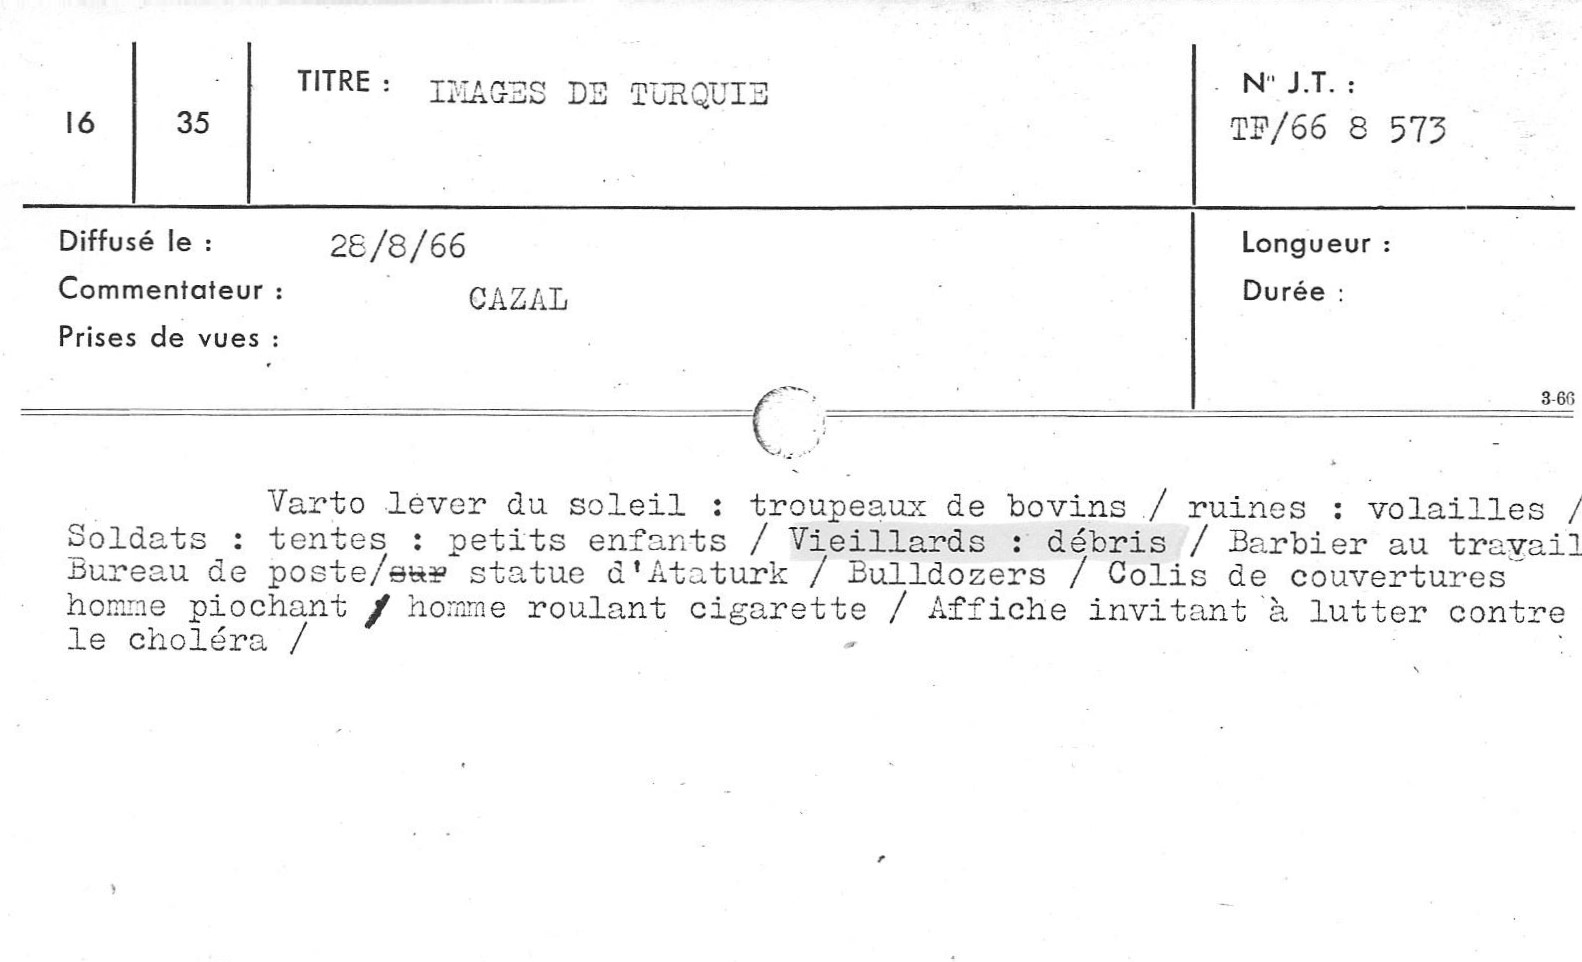
\includegraphics[width=1\linewidth]{./illustrations/notice_turquie_papier.jpg}
	\caption{Photocopie de la notice physique de la notice \enquote{Images de Turquie}}
	\label{fig:imgturquie}
\end{figure}

Pour finir, nous pouvons souligner que ces fiches ayant fait l'objet d'une reprise d'antériorité écrasent les fiches précédentes. L’indexation utilisée pourraient pourtant trouver une valeur aujourd'hui et contribuer à définir une cartographie des traitements documentaires. Au contraire, dans notre cas, elle la complexifie car cette destruction n'est pas systématique à chaque période non plus. Les fiches papiers datant d'avant 1975 ont été conservées par l'INA, certaines sont conservées dans les locaux de l'INA à Bry-sur-Marne, d'autres au centre de conservation de l'INA à Saint-Remy-l'Honoré. Les fiches papiers crées après 1975 ont elles été détruites et la seule trace de leur existante figure dans le champs \enquote{notes} de la notice, indiquant que cette notice a été reprise à telle année\footnote{(Voir entretien d'une documentaliste de l'INA sur l'impact de la politique documentaire sur les données de description ~\ref{ann:transcriptions},\nameref{ann:transcriptions}), p.~\pageref{ann:transcriptions}.}.

\begin{figure}[H]
	\centering
	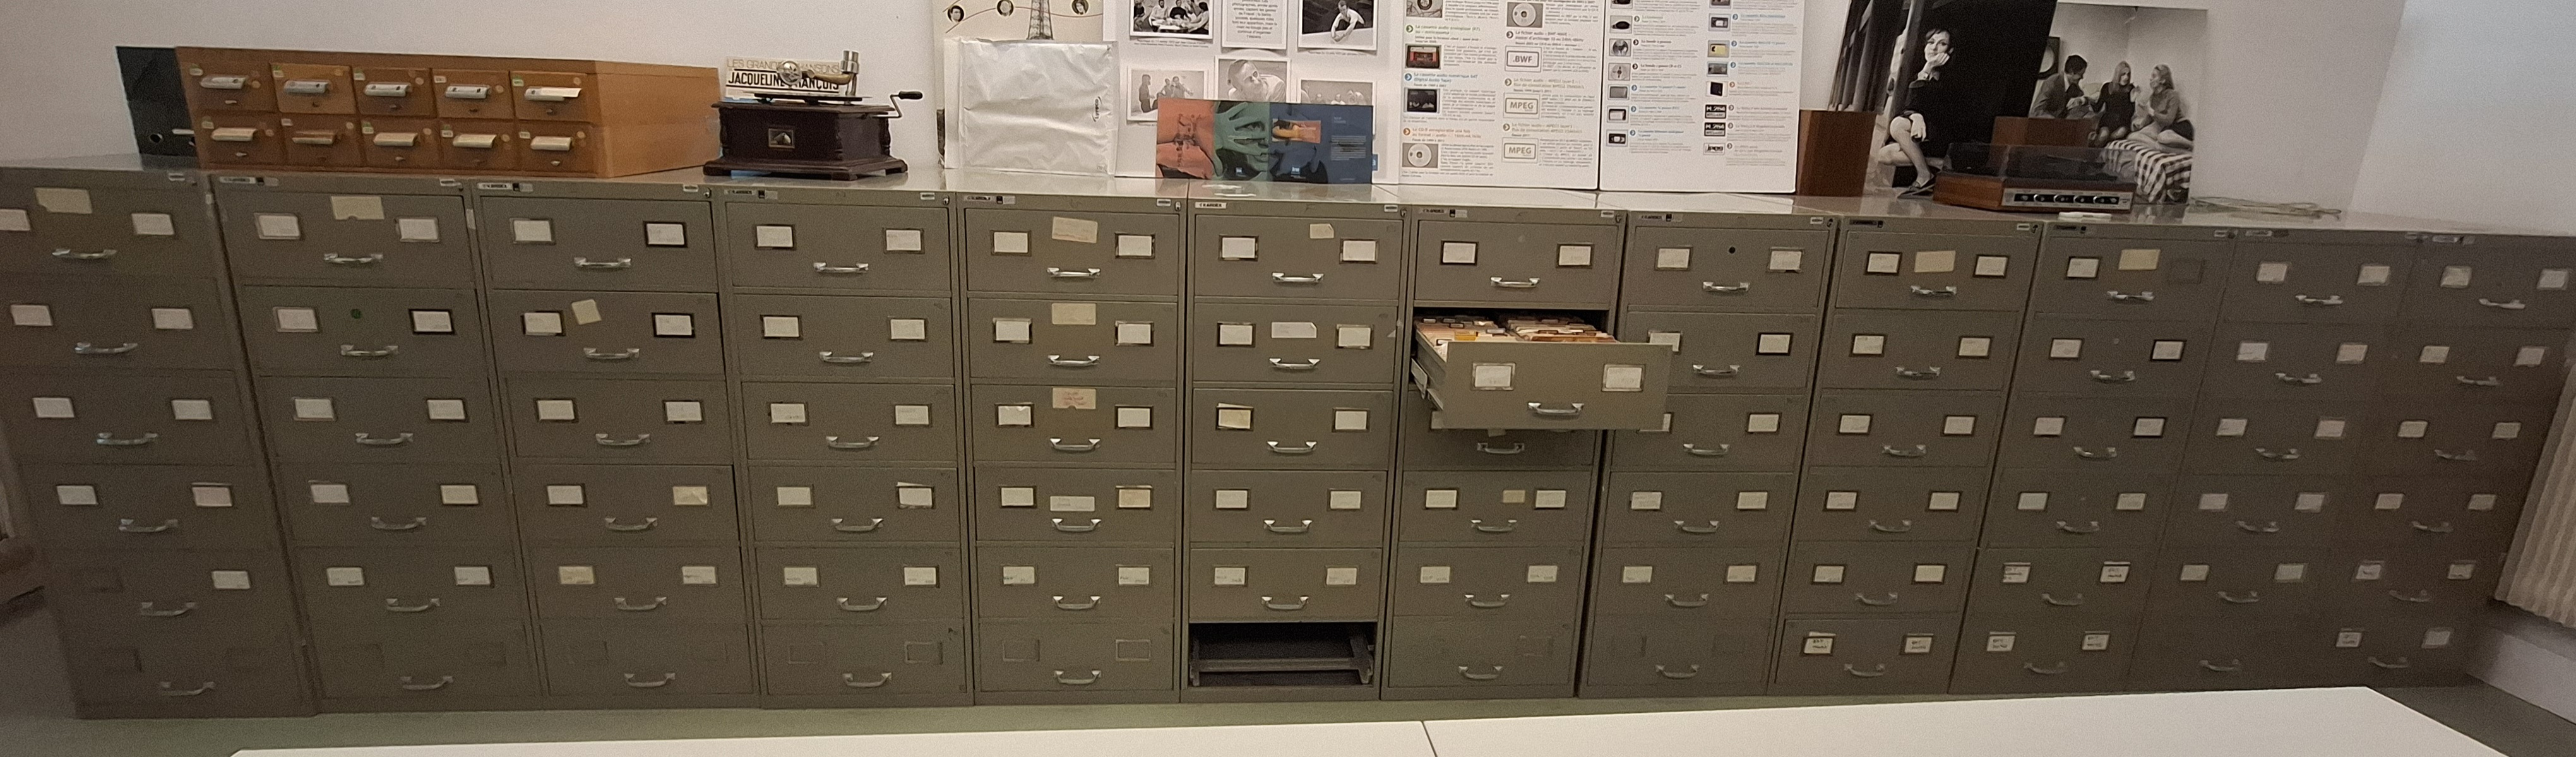
\includegraphics[width=1\linewidth]{./illustrations/tiroir_bry.jpg}
	\caption{Tiroir de classement de fiche papier conservés à Bry 1}
	\label{fig:imgtiroirbry}
\end{figure}

Nous soulevons ainsi un premier obstacle à la compréhension des bases de données. Des notices correspondant à au minimum deux politiques documentaires cohabitent, une politique commerciale et une politique patrimoniale. Les campagnes de reprises d'antériorité sont nombreuses et peu documentées. De plus, certaines notices, considérées lacunaires sont parfois reprises par des documentalistes au cas par cas, parfois sur le signalement de professionnels de l'audiovisuel via la plateforme inamediapro.fr\footnote{(Voir entretien de Pascal Lebeurier sur les outils et services de l'INA ~\ref{ann:transcriptions},\nameref{ann:transcriptions}), p.~\pageref{ann:transcriptions}.}, ce qui diminue une fois de plus le lisibilité des collections dans les bases de données. 

En abordant la reprise d'antériorité comme première approche de la politique documentaire qu'apporte le dépôt légal, nous pouvons souligner l'importance que prend le choix. Un nouveau regard se pose sur les contenus qu'ils conservent et l'usage dont on pourrait en faire. On questionne ce que les publics attendent, les informations qui pourraient les intéresser. Bien que ces reprises concernent également les archives professionnelles, la politique documentaire doit désormais convenir à d'autres publics, différent de ceux qui ont produit ces fiches. L'éloignement temporel que l'institution prend avec ses première notices de description et l'instauration du dépôt légal donnent une place importante à la patrimonialisation de leurs documents. Il n'est plus question de les conserver pour être réutilisé dans un temps court par un public qui connaît ces collections et sa description mais bien pour être communiqué, sur le temps long, autant à un public externe qu'à un public interne n'ayant pas conçu ces descriptions. L'importance du choix dans ces politiques consiste donc à déterminer, à prévoir les informations que l'on souhaitera voir ressortir. Cette notion est particulièrement importante quand on considère que le périmètre du dépôt légal s'étend, accentuant l'importance du choix des contenus à décrire et des informations à inscrire sur ces fiches. 

\subsection{Les types de traitements documentaire}

Il n’est plus question de sélectionner les informations que l’on écrit dans les notices selon le temps dont on dispose mais de sélectionner parmi une grande quantité de données, quelles émissions méritent d’avoir une notice plus fournie qu’une autre. Auparavant, il est essentiel de rationaliser, les 28 millions d’heures captées au titre du dépôt légal évoquées plus tôt. Parmi elles, une partie outrepassent les obligations du dépôt légal mais pour mieux comprendre quelles émissions sont comprises dans le cadre du dépôt légal, il faut revenir à ses tout débuts, avant que les avancées technologiques ne permettent de capter une centaine de chaînes 24 heures sur 24. A ses débuts, le dépôt légal était un \enquote{dépôt} au premier sens du terme et c’était aux chaînes de télévision de déposer leurs émissions, qui étaient ensuite décrites par les documentalistes. Les émissions déposées étaient les émissions de production française diffusées pour la première fois. Ces émissions étaient et sont toujours les émissions décrites. Aujourd’hui, toutes les heures de diffusions captées au titre du dépôt légal sont conservées par l’INA mais seules les premières diffusions de production françaises sont décrites. Ainsi s’opère une première différence concernant les informations de descriptions des émissions. Si l’émission a été captée mais qu’elle ne répond pas à ces premiers critères pour être décrites par un ou une documentaliste, les données de descriptions dans la base de données correspondent aux imports de documentation externe à l’INA. Ils comprennent les grilles du programmes télé\footcite[Pour exemple :][]{admin} ou encore des informations sur les audiences\footcite[Pour exemple :][]{sensio}. Ces données sont rentrées, complétées et vérifiés par des TGDM, des Techniciens de gestion de données multimédia. NB : Revoir pour définition plus précise. 

La réflexion sur le traitement documentaire ne s’arrête pas là car il reste une quantité conséquente de données qui ne peuvent pas toutes êtres prises en charges. S’effectue alors une sélection des émissions sur lesquelles un traitement plus conséquent sera effectué. Loin d’être exceptionnelle, ce choix a déjà été effectué par la BNF, qui pour faire face à une quantité de données numériques massive applique par exemple un traitement moins poussé aux manuels scolaire, considérés moins pertinent pour la recherche\footcite[][70]{bermès2024}. A l’INA, le traitement documentaire est divisé en plusieurs types, identifiés par des codes. La liste qui suit les décrit, en excluant les données de description déjà présentes dans les types de traitements précédents :
\begin{itemize}
	\item \textbf{IDENT}, pour \textbf{identification} correspond à l’absence de traitement documentaire, les notices correspondant à ce traitement doivent comprendre, grâce aux imports : le titre, le générique correspondant aux personnes ayant participées à l’émission, devant ou derrière la caméra, la typologie de l’émission (Journal Télévisé, Documentaire etc\dots) et la nature de production (si l’émission est produite par la chaîne de diffusion ou non).
	\item \textbf{CATS}, pour \textbf{Catalogage signalétique} présente strictement les mêmes informations que IDENT mais vérifiées par un ou une documentaliste. C'est à partir de ce type de traitement que l'on considère que nous nous situons dans du traitement documentaire à proprement parlé car il y a l'intervention d'un ou d'une documentaliste.
	\item \textbf{CATED}, pour \textbf{Catalogage avec descripteurs}. Ce traitement ajoute les descripteurs, correspondant à des mots clés.
	\item \textbf{CATSY}, pour \textbf{catalogage synthétique}. Il ajoute un « chapeau », résumant le contenu de l’émission et le type d’images diffusées.
	\item \textbf{CATA}, pour \textbf{catalogage analytique} auquel s’ajoute un résumé dans lequel sont décrites les principales séquences et une liste des intervenants dans l’émission si il excèdent 5.
	\item \textbf{IND}, pour \textbf{Indexation de contenu} qui propose un résumé plus précis avec une description chronologique détaillée des différentes phases de l’émission, presque au plan par plan\footnote{(Pour plus de détail, consultez la fiche d'aide au dépôt légal ~\ref{ann:aidedl},\nameref{ann:aidedl}), p.~\pageref{ann:aidedl}.}.
\end{itemize}

C’est au cœur de l’utilisation de ces types de traitement que né le projet de cartographie du traitement documentaire. En effet, il n’y a pas, avant la naissance de ce projet, de récapitulatif clair et complet de la chronologie des traitements appliqués aux chaînes et aux émissions captées au titre du dépôt légal par l’INA. La sélection est faites selon les usages que l'on fera de ces images et des ressources que nécessitent leur traitement mais ces informations sont transmises par mails et ces derniers sont finalement perdus dans des boîtes mails personnelles ou supprimés. Le savoir sur la chronologie des applications de traitements repose donc en partie sur les souvenirs des documentalistes \footnote{(Voir entretien d'une documentaliste de l'INA sur l'impact de la politique documentaire sur les données de description qui évoque le traitement documentaire de \enquote{Soir 3} mais qui demande de ne pas trop d'appuyer sur ce savoir étant donné que cette information remonte au début de sa carrière ~\ref{ann:transcriptions},\nameref{ann:transcriptions}), p.~\pageref{ann:transcriptions}.}. De plus certaines considérations se perdent. Par exemple, malgré le fait que les traitements CATS sont considérés comme du traitement documentaire car cela suppose qu’un documentaliste vérifie les informations, dans les faits, le temps manque pour ces vérifications. C’est pourquoi, lors des réflexions de ce projet de cartographie du traitement documentaire, il a été décidé que les notices CATS ne seraient pas comprises dans ce que nous considérons comme du traitement documentaire\footnote{(Voir Cahier des charges du projet de cartographie du traitement documentaire ~\ref{ann:cdc},\nameref{ann:cdc}), p.~\pageref{ann:cdc}.}. Pour appuyer ces considérations, les notices de types IND sont assez rares et ont été progressivement abandonnées dans les années 90 pour des raisons d’économie de temps. Ainsi, même si une personne effectuant des recherches dans les bases de données décide de rechercher les notices IND car il recherche des descriptions très précises, au plan par plan, des émissions, il risque faire ressortir très peu de résultats. Surtout dans une temporalité plus récente, et il ne pourra pas comprendre pourquoi. Pour terminer sur ces défauts dans l'utilisation des types de traitement documentaires, certaines informations ne sont pas transmises au même moment aux documentalistes et aux TGDM, chargés de déterminer quel traitement documentaire est appliqué à une émission donnée. De cette façon, certaines émissions peuvent être indiquées d’un type de traitement en particulier mais ne pas avoir été décrit par un.e documentaliste, voire pas décrit du tout. 

Si nous ajoutons les notices précédant la mise en place du dépôt légal et de ces différents types de traitement, nous commençons à visualiser les problèmes qui s’opposent à la pleine compréhension des bases de données de l’INA pour un public extérieur autant que pour un primo-arrivant à l’INA. En prenant place à l'INA, le dépôt légal entraîne une réflexion sur le traitement documentaire, les politiques documentaires reflètent cette évolution en questionnant les informations qui doivent être renseignées en fonction de différents critères visant à mettre en avant les informations dont les chercheurs, nouveaux public de l'INA aurait besoin. Cette réflexion n'est pas la seule influence qu'a eu le dépôt légal sur le traitement documentaire. A un niveau strictement humain, l'INA divise ses services de traitement de ses collections en deux. Cela entraînera un déséquilibre dans le traitement documentaire qui plus de 30 ans après la création du dépôt légal a toujours des conséquences majeure sur l'accessibilité aux collections. 
	 
	\section{Impact des changements institutionnels : le facteur humain dans les données}
	
	%% Introduction %%

Bien que ces deux deux services suivent les mêmes missions de conservation et communication, ils s'opposent à plusieurs niveaux. Là où le dépôt légal applique ces missions aux documents captés ou déposés au titre du dépôt légal, le service des archives professionnelles concerne la conservation et l’exploitation commerciale des archives de l’ORTF et les archives confiées par la loi à l’INA sur lesquels l’institution a un droit d’exploitation. Au delà de leurs fonds, ces services s'opposent aux archives du dépôt légal dans leur organisation. Les archives professionnelles fonctionnent en « stock », elles gèrent des stocks, des programmes, des émissions à l’unité, qu’elles exploitent, au contraire du dépôt légal qui a une gestion en « flux », selon les tranches horaires, les grilles de programmes\footcite[][23]{varra2023}. Les archives professionnelles conservent un programme dans la meilleures qualité possible, le dépôt légal le conserve autant de fois qu'il a été diffusé. C'est la manifestation des publics et usages différents qu'ils servent et que nous avons déjà évoqués plus tôt. Les archives professionnelles communiquent avec les professionnels de l’audiovisuel : les chaînes de télévisions, les journaux télévisés, ils ont donc besoin d'accéder à leur contenu par sujet, par programme unique. Le dépôt légal communique avec les chercheurs de l'INAthèque, qui peuvent aussi bien travailler sur un programme que sur une chaîne ou sur une tranche dans leur ensemble. Pour répondre à ces usages différents, les deux services adoptent deux politiques documentaires différentes. 

\subsection{Des données de descriptions divergentes}

Aujourd’hui, ces deux services ont disparu à la suite de plusieurs réorganisations des services, dont la dernière, en 2020, qui répartit ces deux services dans la « Direction des Patrimoines »\footnote{(Voir organigrammes de la direction des Patrimoines :~\ref{ann:org},\nameref{ann:org}), p.~\pageref{ann:org}.}. Cependant, ils transparaissent toujours de diverses manières au sein de la politique documentaire en vigueur. Nous avons déjà vu que leurs objectifs et leur public n’était pas les mêmes, mais nous n’avons pas vu de quelle façon cela se répercutait sur le traitement documentaire. Pour illustrer nos propos, prenons pour exemple deux notices d’une même émission\footnote{(Pour consulter les notices voir :~\ref{ann:notices},\nameref{ann:notices}), p.~\pageref{ann:notices}.}, une notice provient de Totem, l'outil de consultation de la base de données des archives professionnelles, l’autre vient de DLTV, la base de données du dépôt légal. Évidemment, les deux notices présentent des informations de description identiques telles que le titre, la date de diffusion, le genre d’émission, le générique et même le sommaire. Mais les informations sur la diffusion diffèrent. Du côté professionnel, nous trouvons la date, l’heure mais l’information importante du côté dépôt légal est que cette émission est en première diffusion. Cette information a peu de valeur dans le cadre d’une commercialisation mais elle en a une à la fois pour les TGDM chargés de déterminer le type de traitement à appliquer à cette émission et pour les chercheurs de l’INAthèque. Les autres informations de diffusion sont présentes dans la fiche Hyperbase mais elles sont réparties entre différents champs afin de permettre la recherche par ce champ. Les autres données de description le confirment. Dans la fiche des archives professionnelles, nous retrouvons les informations concernant le statut de numérisation, essentiel pour partager ce document, la dévolution, sur laquelle nous allons revenir, et surtout des informations précises sur les fichiers, pour la diffusion de ce document. Toutes ces informations sont absentes de la fiche du dépôt légal. Au contraire, nous trouvons dans la fiche du dépôt légal des informations sur les documents d’accompagnements, pouvant compléter une recherche et les audiences permettant, entre autres, de réaliser des statistiques. Usage courant pour un chercheur mais improbable pour un professionnel de l'audiovisuel.

\subsection{Un fossé entre les services de conservation} 

En comparant ces deux fiches, il est évident que même actuellement, des années après la réorganisation des services, deux politiques documentaires cohabitent. Pourtant, l’écart entre les deux services patrimoniaux est bien moins important qu’il ne le fut. À la création du dépôt légal, il est nécessaire de trouver de nouveaux locaux pour accueillir ce nouveau service. Le service du dépôt légal investit des locaux à une centaine de mètres des locaux historiques de l’INA à Bry-sur-Marne\footcite[][24]{varra2023}, creusant un fossé entre les deux services, même physiquement. C’est un ressenti évoqué par une documentaliste interrogée, anciennement au dépôt légal, qui souligne l’écart entre les deux services. L’accès aux notices, aux images et aux sons des documents du service des archives professionnelles étaient compliquées avant leur numérisation car ils n’avaient même pas accès à l'outil de consultation du service\footnote{(Voir entretien d'une documentaliste de l'INA sur la différence entre le dépôt légal et les archives professionnelles~\ref{ann:transcriptions},\nameref{ann:transcriptions}), p.~\pageref{ann:transcriptions}.}. Dans ces circonstances, on peut difficilement imaginer une bonne communication sur les politiques documentaires. D'autant plus que ce n'était pas la première fois de l'histoire de la conservation des documents audiovisuels que différents services de l’INA furent séparés géographiquement. Avant même sa création, la cinémathèque était séparée entre les services « Film d’Actualités » à Cognacq-Jay et « Film Production » aux Buttes Chaumont. Ils seront réunis pour une courte durée à la création de l’INA, à l'occasion de laquelle ils réunissent leur fiches papiers, non sans difficulté\footcite[]{saintville1994}, avant de se séparer à nouveau puis d’être réunis à Bry-sur-Marne. Nous pouvons donc imaginer, en conséquence, les nouvelles incohérences générées dans les politiques documentaires. Une fois de plus, nous savons qu'elles existent, mais difficile de pointer avec exactitude lesquelles sont affectées tant la communication étaient compromises et l'archivage des pratiques documentaires absentes. 

Nous pouvons terminer en soulignant toutes les erreurs d'origine humaines : fautes de frappes, erreurs d'orthographes notamment des noms, omission volontaire ou non. Le contexte de description de ces notices peut également avoir un impact. Dans le cas des prises d'antenne, si une grève a lieu, il n'y a pas de description et d'indexation. Certaines notices sont indiquées \enquote{non indéxé parce qu'en grève}\footnote{(Voir entretien d'une documentaliste sur l'impact de la politique documentaire sur les données de description~\ref{ann:transcriptions},\nameref{ann:transcriptions}), p.~\pageref{ann:transcriptions}.}. Cela dit, le manque de communication n’est pas ignoré, à plusieurs reprises, il sera tenté d'harmoniser les méthodes. Des référentiels, des thésaurus sont mis en place nous pouvons plus particulièrement souligner la création de la DDCOLL, direction déléguée des collections, en 2010 qui met en place une structure transversale « méthodes et qualités » et qui donne lieu à la réunification des services, évoqués plus haut\footcite[][29]{varra2023}, ainsi que la création du « lac de données » sur lequel nous reviendrons. 

%% Conclusion %%

Ces perturbations d’ordre institutionnel ne trouvent pas leur pareil au sein des institutions patrimoniales ayant pour mission le dépôt légal. Il n’y ni au sein du CNC, ni au sein de la BNF de distinction entre les documents du dépôt légal et les documents commercialisés. C’est une exception que l’on doit au statut d’EPIC (Établissement public à caractère industriel et commercial en France) de l’INA que l'on ne retrouve pas à la BnF ou au CNC. Cette exception est responsable de cet écart actuel entre le traitement documentaire réalisé sur des archives professionnelles et celui sur les archives du dépôt légal. C'est aujourd'hui un enjeu d'accessibilité car il peut-être difficile de savoir quelles informations peut-on trouver et où ? 
	
	\section{Impact du contexte économique}
	
	%% Introduction %%

L'aspect monétaire n'a pas seulement un impact sur le traitement documentaire dans le cadre de la commercialisation des archives professionnelles comme nous l'avons démontré plus tôt. A plusieurs reprises le manque de moyen eu un impact sur des politiques documentaires. 

%% Recyclage des bobines %%
\subsection{Économie de matériaux}

A commencer par le tout début de la conservation des documents audiovisuels télévisés. Les moyens manquaient et il était courant de recouper les bobines pour utiliser la bande restante ou pour les faire fondre afin de récupérer l'argent qui couvre les pellicule ou les recycler. C’est une problématique déjà importante pour les archives du cinéma. Pour les archives de la télévision, c’est ce qui motiva Violette Franck à conserver ces documents. C’est cette décision qui donnera naissance à la cinémathèque de l'ORTF et plus tard l’INA. Sans cette héroïne des temps modernes nous pouvons supposer que ces documents auraient connus le même sort que les débuts de la radio en France dont il est périlleux de trouver des traces avant 1944\footcite[14]{jean-michel1986} ou encore des débuts des radios libres, presque impossible à consulter\footcite[16]{jean-michel1986}. De même que dans les débuts du cinéma où les supports de films n'étaient guère considérés que comme des consommables, abandonnés dans des hangars dès l'instant où ils deviennent inutiles, usés jusqu'à la dégradation pour rentabiliser chaque seconde d'image ou découpés, comme le fut la télévision pour recycler les précieuses bandes\footcite[][28]{olmeta2002}. Nous pouvons même nous aventurer aux Etats-Unis où les bandes ont connus cette même menace du coup de ciseau pour économiser les bandes d'enregistrement\footcite[17]{zotero-item-763}. Pour autant beaucoup de documents des débuts de la télévisions ont disparu. C'est ainsi que même aujourd'hui, beaucoup de documents, d'émissions diffusées par l'ORTF manquent toujours. 

%% Stock Gambais %%
\subsection{Le stock Gambais}

Dans ce cadre, le \enquote{stock Gambais} se revêt d'une importance capitale. C'est le nom que l'on donne aux quelques 160 000 boîtes de supports physiques d'archives audiovisuelles retrouvées dans un ancien hangar de l'ORTF à Gambais et aujourd'hui stockés au centre de conservation de Saint-Remy-l'Honoré\footcite[]{theque2024}. Depuis sa découverte au début des années 2000, c'est un travail de longue haleine qui s'est engagé pour dépouiller chaque support et vérifier dans les fonds de l'INA si c'est un document manquant ou si la version retrouvée est de meilleure qualité. De nombreux extraits et programmes complets furent retrouvés ainsi, y compris un fond importants d'émission d'outre-mer, négligés par le traitement documentaire. C'est ainsi que de nouveaux, notices anciennes et récentes se mélangent, entre les notices de documents datant de l'ORTF, documents ayant fait l'objet d'une reprise documentaire et documents issus du stock Gambais, ou repris lors de la découverte d'une meilleure copie. Ainsi, même quand un ou une documentaliste met en garde un chercheur de l'INAthèque contre les documents antérieurs à 1975 pour leur absence de mots clés\footnote{(Voir entretien d'une documentaliste de l'INA sur l'expertise du documentaliste~\ref{ann:transcriptions},\nameref{ann:transcriptions}), p.~\pageref{ann:transcriptions}.}, il y a toujours plusieurs couches d'informations à prendre en compte lors d'une recherche dans les fonds de l'INA. 

%% Coupures budgétaires %%
\subsection{Un budget contraignant}

Pour finir, certaines décisions furent prises pour des raisons financières, notamment dans le cas des types de traitement IND que l'on a cessé d'utiliser pour des raisons de temps et par extension, de budget. Les documentalistes et leur temps sont une ressource précieuse. Il en est finit de recruter en masse des documentalistes comme ce fut le cas à la création du dépôt légal, ce temps doit donc être alloués à ce qui rapporte potentiellement le plus. Ce manque de temps opposé aux quantités de données de plus en plus importantes se ressent dans les politiques documentaires. A partir de 2019, le type de traitement appliqué à un document commence à être déterminé selon son appartenance au fonds dévolu à l'INA. Nous appelons fonds dévolu un fonds incluant les documents pour lesquels la loi a substitué les droits et obligations des sociétés nationales de programme à l'INA (ou le cas échéant à une institution donnée). L'institut a donc tous les droits pour exploiter ces documents. Le fait de déterminer le traitement documentaire sur l'appartenance du document à ces fonds signifie que les documents desquels l'institution peut réaliser un profit aura une description plus appliquée. L'aspect économique prend donc une telle importance qu'il affecte le traitement documentaire du dépôt légal en priorisant une fois de plus l'aspect financier sur le patrimoine. En contrepartie, le traitement de ces émissions repose de plus en plus sur les TGDM, chargés d'ajouter les imports de données, qui voient progressivement s'élargir leur périmètre d'action. Par exemple, récemment, le traitement documentaire de la chaîne France 2 s'est arrêté au profit du traitement des documentalistes de la chaîne télévisées. Il y a certes toujours l'action d'un.e documentaliste et ils utilisent les mêmes référentiels mais les pratiques ne sont pas tout à fait les mêmes, ils ne donnent pas la priorité aux même termes, par dans le même sens car leur mission n'est pas la patrimonialisation en priorité. La nécessité de commercialisation et de rentabilité s'oppose à la communication patrimoniale. 

%% Conclusion %%

L'aspect économique n'influence pas le traitement documentaire de la même façon que le font les usages du traitement documentaire. Il ne contraint les champs descriptifs des documents mais il contraint le périmètre du traitement. Plus les conditions économiques sont favorables, plus le temps des documentalistes est généreusement distribués et plus le périmètres de l'application du traitement documentaire est large et plus il est précis. Cela compromet l'accessibilité aux collections car il n'est pas envisageable de demander à utilisateur des bases de données de l'institution, quel qu'il soit de connaître ces aléas et de comprendre en quoi il affecte son expérience. Cela rejoint le constat que nous avions déjà effectué selon lequel l'accessibilité est compromise par plusieurs facteurs empêchant l'utilisateur de comprendre quelles informations ils peut trouver dans ces bases de données. 
	
\chapter{Une informatisation du patrimoine}

	\section{Documentation et informatisation : discipline historique et nouvelles technologies}
	
	%% Introduction %%

Pour compléter notre propos, il est essentiel de comprendre que ces changements s'accompagnent d'une informatisation progressive des institutions patrimoniales et en conséquent du traitement documentaire. En effet, dans les années 70, la société s’informatise progressivement et l’INA ne fait pas exception. Elle se dote de ses premières bases de données et des questionnements documentaires qui les accompagne. 

\subsection{Histoire de la documentation}

%% Introduction %%

Pourtant, il est essentiel de ne pas négliger que ces questionnements sur le traitement et la politique documentaire n’ont pas attendu l’informatisation de la société pour être posée. Bien au contraire, ces nouvelles réflexions reposent sur des bases posées dès la naissance des livres imprimés. Pour comprendre les décisions prisent pour le traitement documentaire à la création de la cinémathèque puis à l'instauration du dépôt légal, il est important d'en comprendre les origines, les premières définitions et premières réflexions. Ils ont ouvert la voie à la mise en place d’outils et de techniques d’accès à l’information desquels les outils que nous utilisons aujourd'hui sont les héritiers. 

%% Naissance de la documentation %%

Ils naissent d’abord dans des cercles privés, avant de devenir collectifs\footcite[][15]{fayet-scribe2000}. Pour le constater, il nous suffit de nous plonger dans les origines de la BNF, quand à la révolution française Lefèvre d’Ormesson lance le projet de Bibliographie universelle de la France qui vise à constituer un inventaire des livres de la nation française, c’est à cette période que naît le terme « documenter », reprenant le sens ancien du terme « documenter » soit instruire et enseigner. A l’occasion de cette bibliographie nationale on y interroge également pour la première fois « l’ordre des connaissances »\footcite[][21-22]{fayet-scribe2000}, soit l’organisation des savoirs, comment réunir ces documents par les connaissances qu'ils renferment. 

%% Paul Otlet %%

En 1895 est crée à Bruxelles l’Institut international de bibliographie grâce à Paul Otlet et Henri Lafontaine. Ils sont considérés comme les créateurs de ce nouveau domaine qu’est la documentation\footcite[][45]{fayet-scribe2000} dont ils définissent le périmètre : 
\begin{displayquote}
	[…] des méthodes seront trouvées pour dépouiller les ouvrages avec suite et ensemble et permettre de retrouver instantanément, sans peine ni difficultés, les matériaux mêmes dont chaque publication fait apport à l’ensemble du savoir\footcite[Paul OTLET, « Les sciences bibliographiques et la documentation », Bulletin
	de l’IIB, 1903, pp.125-147. Retranscrit dans][48]{fayet-scribe2000}
\end{displayquote}
A cette occasion ils se séparent de la matérialité du manuscrit pour parler d’un « document », qui sert diffusent des informations, quelles que soient leur forme\footcite[][49]{fayet-scribe2000}. Cette définition trouve toujours un sens aujourd'hui. Nous utilisons au long de ce mémoire le terme général de \enquote{document} pour parler des images et sons conservés à l'Institut National de l'audiovisuel. Ces \enquote{documents} permettent de diffuser des informations, quelles qu'elles soient et nécessitent d'être organisés de façon à ce que tout un chacun puisse avoir accès aux connaissances qu'ils renferment. La documentation doit savoir s’adapter, peu importe la forme que prend le document et fournir toutes les informations permettant son identification et son partage\footcite[][55]{fayet-scribe2000}. Son projet se matérialisera en France à travers Charles Gariel et le général Hippollyte Sebert avec le Bureau bibliographique de Paris (BBP), branche française de l’Institut international de bibliographie\footcite[][62]{fayet-scribe2000}. Dans un objectif de normalisation, ils appliquent le classement décimal et naîtra en 1926 l’AFNOR, l’Association française de normalisation\footcite[][79]{fayet-scribe2000}. Paul Otlet et Henri Lafontaine poseront donc une base solide de l’institutionnalisation et l’internationalisation de la documentation des « documents ». Par cette internationalisation établissent l'importance de permettre le partage des description documentaire.

%% Suzanne Briet %%

A sa suite, Suzanne Briet, représentante de la Bibliothèque nationale au Bureau Bibliographique de Paris à partir de 1932. Elle constatera à la bibliothèque nationale que les outils documentaires mélanges nouveaux et anciens usages. En conséquent, elle créera un fichier d’information à l’attention des lecteurs afin de rassembler l’ensemble des catalogues, répertoires et bibliographies à leur disposition\footcite[][129]{fayet-scribe2000} et contribuera à l’ouverture de la salle des catalogues et des bibliographies à la bibliothèque nationale. Elle appuie ainsi l'importance de permettre aux chercheurs de comprendre ce que l'on pourrait appeler \enquote{l'architecture} du traitement documentaire auxquels ils sont confrontés. En ce sens, notre projet de cartographie du traitement documentaire de l'INA peut être rapproché de son projet. Tous deux ont pour volonté de donner toutes les clefs nécessaire aux chercheurs et plus largement aux utilisateurs des collection d'une institution patrimoniale pour réaliser la recherche la plus complète possible dans le catalogue de ces collection. En cela, le documentaliste est placé comme la clef du partage de ce savoir. Dans son manifeste « Qu’est-ce que la documentation ? », elle définit ainsi le métier de documentaliste : 
\begin{displayquote}
	1° est un spécialiste du fond, c’est-à-dire qu’il possède une spécialisation culturelle apparentée à celle de l’organisme qui l’emploie ; - 2° connaît les techniques de la forme des documents et de leur traitement (choix, conservation, sélection, reproduction); - 3° a le respect du document dans son intégrité physique et intellectuelle; - 4° est capable de procéder à une interprétation et à une sélection de valeur des documents dont il a la charge, en vue d’une distribution ou d’une synthèse documentaire.\footcite[][19]{briet}
\end{displayquote}
Définition qui plus de 70 ans plus tard entre toujours en résonance avec le métier de documentaliste actuel, malgré toutes les mutations que ce métier a connu. 

Nous distinguons déjà, dans ce même manifeste, les prémices de la transformation majeure que s’apprête à connaître le traitement documentaire : 
\begin{displayquote}
	A côté des fichiers et des catalogues qui présentent l’image schématisée des documents, par description abstraite de leur aspect formel, accompagnée ou non de photographie, on voit depuis peu de temps se constituer des fichiers parallèles obtenus par codification des éléments pouvant donner lieu à statistique ou à sélection. Le mot ici disparait, la lettre même est parfois absente, lorsque l’on a affaire aux machines à cartes perforées. La mécanographie statistique nous habitue à doubler les fichiers lisibles en clair par des fichiers où chacune des notations est la traduction conventionnelle des signes directement intelligibles. […] Le documentaliste sera de plus en plus tributaire d’un outillage dont la technicité augmente à une vitesse grand V. L’homo documentator doit se préparer à commander, toutes facultés en éveil, aux robots de demain\footcite[][28]{briet}.
\end{displayquote}

%% Rapprochement des disciplines %%

L’Histoire de la documentation et du traitement qui s’en accompagne est encore doté de plusieurs figures importantes et nous pouvons toujours y trouver des échos à la discipline que nous connaissons aujourd’hui. Tout au long de son évolution s’est toujours posé la problématique d’allier nouveaux et anciens outils. C’est une problématique à laquelle les institutions patrimoniales n’échapperont pas non plus. En 1993, Michel Melot, président du Conseil supérieur des bibliothèques évoque comme les disciplines propre aux bibliothèques, archives et documentation sont en train de se rapprocher grâce à la numérisation :
\begin{displayquote}
	La numérisation réduit tous les documents au même dénominateur commun, au même support physique. Nous entrons dans l'ère de l'unimédia. [...] 
	Bibliothèques et archives se rapprocheront. Quand les documents issus de la marche d'un service ou d'une entreprise seront disponibles sur les réseaux domestiques, la notion d'archives rejoindra celles de l'édition et lorsque l'éditeur sera le propriétaire de bases textuelles stockées sur serveur et accessibles à la demande, la notion d'édition aura rejoint celle des archives. Les accès en texte intégral auront, de même, fait se rejoindre les fonctions bibliothécaires (accès à l'unité bibliographique) et documentaires (accès au contenu des documents)\footcite[]{melot1993}.
\end{displayquote}
C'est en effet ce que nous pouvons constater en nous intéressant à la façon dont l'informatique s'est appropriée la documentation. 

\subsection{Prise en main de la documentation par l'informatique}

Nous pouvons reprendre notre développement aux années 70 et au début de l'informatisation de la société. Les bases de données commencent à être adoptées et comme l’avait introduit Suzanne Briet, ces « fichiers parallèles » s’imposent et les institutions s’adaptent. En 1968 émerge le format MARC (Machine-Readable Cataloging), permettant le stockage et l’échange de notices bibliographique par ordinateur qui sera rapidement adopté par de nombreuses bibliothèques, y compris la BNF. A l’INA, la première base de données est mise en place avant même sa création, par la vidéothèque de production. Nommée MIOR, elle garde toujours la structure de leur catalogue papier dans la continuité de ce mélange d’anciens et de nouveaux outils. Tout comme le système IMAGO en 1975, qui n'est pas une base de données à proprement parlé. Cette première version d’IMAGO est adaptée au thésaurus de l’INA et centralise toutes les collections qu’elle conserve\footcite[][42-44]{bassaïstéguy2025} mais elle reste toujours très attachée à la logique d’un catalogue de bibliothèque. Les notices étaient dans un premier temps saisies sur papier par les documentalistes puis saisies informatiquement par des prestataires. Deux fois par mois des index titres, générique et analytique étaient imprimées sur microfiche, ce qui se révéla néfaste pour certains champs du générique qui n'apparaissaient sur une seule émission d'une série pour gagner de la place\footcite[]{saintville1994}. La deuxième version d'IMAGO, en 1985 s’éloigne un peu plus des catalogues de bibliothèque grâce à différentes normes mises en place par la Fédération internationale des archives du film (FIAF), les \textit{Cataloging Rules for Film Archives}, pensées pour s’adapter à l’informatisation des catalogues de documents audiovisuels et permettre leur partage\footcite[][50]{bassaïstéguy2025} ainsi que par l'AFNOR avec les premières normes de l'image animée auxquelles l'INA a participé\footcite[]{saintville1994}. Nous pouvons souligner le parallèle avec l’importance que Paul Otlet donnait à l’internationalisation des normes de documentation. L’évolution des moyens informatiques y prend également une grande importance, les données sont transférées dans une base de données Mistral. Ce nouveau système permet cette fois la saisie en temps réel, la gestion informatisée des supports d'archives et la recherche documentaire\footcite{saintville1994}. Avec cette deuxième version, nous pouvons pour la première fois parler d'une base de données. 

%% Indexation %%

%En parallèle, les indexations évoluent en fonction des demandes professionnels. La demande de la première apparition d'une personnalité à la télévision revient souvent alors on ajoute l'indexation \enquote{première apparition}\footcite[]{saintville1994}, c'est une indexation adaptée à son public cible.  

%% Impact sur le traitement documentaire

Dans la chronologie des outils de consultation des documents conservés par l’INA, nous nous situons désormais à l’aube du dépôt légal et pourtant, l’arrivée de l’informatisation à l’INA génère déjà les premiers défauts dans les données de description. En passant d’IMAGO I à IMAGO II, certains champs ne correspondent plus. Quand les notices d’IMAGO I sont versées dans IMAGO II, les champs titres, sont automatiquement versés dans le champ titre collection, négligeant le titre de tranche horaire ou à un titre propre. Cela concerne potentiellement 230 000 documents réalisés avec IMAGO I. A la fin des versements, cela ne génère pas de problèmes lors de l’interrogation de la base de données car tous les champs titres sont interrogés\footcite[][53]{bassaïstéguy2025}. Mais aujourd’hui ce sont des défauts supplémentaires qui compromettent la recherche dans les bases de données, surtout dans la nouvelle base de données du dépôt légal. Les modalités de recherches dans cette base de données est tout à fait différente de celle de ce que l’on va désormais appeler les archives professionnelles. Les défauts effacés par cet outil de consultation apparaissent parfois bien plus clairement dans la base de données du dépôt légal. Et comme toutes les perturbations que nous avons déjà soulignées dans les données de descriptions dû à différentes politiques documentaires, la connaissance de ces évènements se perdent ou du moins ne se transmettent à chaque personne nécessitant d’effectuer une recherche dans une des bases de données de l’INA et l’accessibilité est largement compliquée.

%% Conclusion %% 

Malgré tout, cette informatisation, qui met à disposition de nouveaux outils pour la documentation de documents audiovisuels se place tout de même en héritier de cette longue histoire de la documentation. Le terme de document reste applicable aux nouveaux supports que conservent l'INA et la place des documentalistes reste essentielle à l'application des politiques documentaires. De même que ces politiques s'appuient toujours sur des normes favorisant le partage de ces documents. Ces outils commencent à particulièrement s'émanciper de leur héritage en s'adaptant aux besoins de leurs utilisateurs. La meilleure façon de mettre cela en avant est de nous intéresser à la création du nouvel outil de consultation et de production pour le dépôt légal. 
	
	\section{Deux logiciels, deux objectifs, une institution}
	
	\subsection{Les outils du dépôts légal : du sur mesure pour la nouvelle mission patrimoniale}

%% Introduction %%

À l'arrivée du dépôt légal, l'INA possède donc déjà un outil pour la gestion des données : IMAGO, mais il est estimé dépassé et trop rigide pour s'adapter à la nouvelle logique du dépôt légal. Il est nécessaire de mettre en place un outil qui convient aux besoins de cette nouvelle mission. 

%% Intégration du logiciel du dépôt légal : Hyperbase %%

On favorise l'utilisation de nouvelles bases de données. Une pour la radio : DLradio, une pour la télévision hertzienne : DLTV, une pour les chaînes du câble, du satellite et de la TNT : DLSat, une pour les chaînes régionales : DLREG. Un nouvel outil de production est mis en place : DLexe et un nouvel outil de consultation de la donnée : Hyperbase. Chaque champ a son référentiel. L'interface a été réalisé en adéquation avec les besoins de l'équipe du dépôt légal. Le dépôt légal fonctionnant en flux et pas en stock comme le font les archives professionnelles, les outils sont de ce fait concentrés sur les chaînes, puis les tranches horaires. Le fonctionnement des outils de production et de consultation devait être élaboré en fonction de ces prérequis. Ils fonctionnent avec trois interfaces : 
\begin{itemize}
	\item Gestion des journées de programmes : Contiennent l'ensemble des émissions d'une tranche horaire. Se présentant sous forme de liste. Aujourd'hui, c'est une fonctionnalité gérée par les TGDM.
	\item Gestion des matériels : Cette fonctionnalité évoluera bien évidemment avec la numérisation mais à la création du dépôt légal, les chaînes déposent encore le dépôt légal en supports physiques. 
	\item Saisie des documents\footcite[]{Rodes1994}
\end{itemize}
La traitement documentaire, quant à lui, se recentre sur la structure de l'émission. Les \enquote{notices de collection}, décrivant une émission, une collection et pas seulement une diffusion prend plus d'importance. Dans la même lignée. Dans l'indexation on donne une grande place à la description de décors techniques. Notion qui n'intéressait les correspondants de chaînes télévisées. 

%% IMAGO III et Totem %%

Les archives professionnelles étant en stock, les outils de production et de consultation de données sont plus concentrés sur l'émission, l’œuvre, le thème. L'unité est à un niveau inférieur à l'émission. La description est concentrée sur le \enquote{sujet} traité par l'émission car c'est ce qui sera recherché. L'indexation décrit avant tout l'image. Ceci dit, il est important de considérer que les notices pour les archives professionnelles ne sont pas créées ex nihilo, elles sont transmises de la base de données du dépôt légal, le traitement documentaire est donc adapté à des fins commerciales. 

\subsection{La recherche au dépôt légal et dans les archives professionnelles}

Ainsi, ces deux outils de consultation ne sont pas construits pour être utilisés de la même façon. Hyberbase, l'outil de consultation à disposition des documentalistes de l'INA et des chercheurs de l'INAthèque est construit pour combiner des requêtes afin de construire un corpus. Dans le sens inverse, \enquote{Totem}, l'outil de consultation et de production qui a succédé à \enquote{IMAGO} est tourné sur la recherche d'images pour les professionnels. Il est déjà organisé en corpus, élaboré par les documentalistes. Il est conçu pour lancer une première recherche que l'on peut affiner par la suite\footnote{(Voir entretien d'une documentaliste sur les bases de données de l'INA~\ref{ann:transcriptions},\nameref{ann:transcriptions}), p.~\pageref{ann:transcriptions}.}. 

Les outils de production des archives professionnelles et du dépôt légal sont particulièrement représentatifs de la séparation du traitement documentaire qui a opposé des années durant les services des archives professionnelles et du dépôt légal. Par leur fonctionnement, ils illustrent l'opposition des politiques documentaires qui ont opposé ces deux services des années durant et il contraignent les utilisateurs des bases de données internes à l'INA à toujours mobiliser ces deux politiques documentaires, ce qui ne facilite pas la compréhension des collections dans leur ensemble, tant elles sont décrites et présentées au public sous différents angles. 

\subsection{Le lac de données}

Cela fait de nombreuses années que l'INA a conscience de ces déséquilibres entrainés par la séparation des services et des outils du dépôt légal et des archives professionnelles. C'est ainsi que né le \enquote{lac de données} en 2015. Il a pour objectif de centraliser l'ensemble des données de l'INA en une seule infrastructure. Cette fois, il n'est plus question d'élaborer les outils en fonction des usages mais en fonction des données\footcite[]{institutnationaldhistoiredelartinha2019a}. En conséquent, un nouveau modèle de données est mis en place dans lequel toutes les données sont misent en relation et tous les référentiels des différents services de l'INA sont repris et mis en commun. Les collections sont divisées en trois entités, elles-mêmes décrites par des métadonnées : le contenu (les images, le son, l'émission en elle-même), l'évènement (date de diffusion, de production etc\dots) et le matériel (le support, le fichier sur qui contient le contenu)\footcite[87]{bassaïstéguy2025}. Ainsi, il doit être plus facile de convenir aux usages des données de tous les services de l'INA. 

Le lac permettrait de résoudre beaucoup des défauts que nous avons constaté précédemment. On opère une migration des données à partir de 2017 vers les nouvelles bases de données et on opère dans le même temps un énorme travail sur la qualité des données. Les données en double sont dédoublonnées, les erreurs corrigées, les données enrichies. Mais aujourd'hui, après plusieurs migrations des métadonnées et référentiels c'est un traitement différentiel qui est mis en place et encore une fois, il marque une différence entre les données du dépôt légal et des archives professionnelles. Aujourd'hui les données de la base de données des archives professionnelles sont synchronisées avec le lac de données toutes les 30 minutes quand ce sont seulement les référentiels du dépôt légal qui sont synchronisés, une fois par jour\footnote{\enquote{Le modèle de données de l'INA}, présentation powerpoint conçue par Axel Roche-Dioré, mis à jour par Soline Doat, 6 novembre 2025.}.  

Malgré les avantages que représente le lac de données pour notre outil, il n'est pour le moment pas possible de le mobiliser sans faire impasse sur une partie des données récentes du dépôt légal, sur lequel repose cette cartographie du traitement documentaire. 
	
	\section{Trop de données tue la données ?}
	
	%% Introduction %%

Pour terminer sur cette accumulation de facteurs résultant en cette absence de visibilité sur le \gls{td} dans les bases de données actuelles de l'INA. Il est important de souligner la quantité massive de données que conserve l'INA. Nous avons déjà évoqué à plusieurs reprises cette quantité massive de données. Afin de comprendre en quoi cela affecte l'accessibilité aux données, nous allons nous attarder dessus un temps. 

 %% Sources des données %%

C'est un fait, l'INA conservent une quantité très importantes de données, elles sont le résultat d'une collecte provenant de sources multiples et très productrice de données. Nous en avons cité les principales avec la captation au titre du dépôt légal, elle enregistre 24 heures sur 24 120 chaînes télévisées, ce qui ajoute aux collections numériques 1 millions d'heures par an.  A cela s'ajoute les fonds de l'ORTF les Actualités françaises, les fonds issus de divers dons, le dépôt légal du web etc... 

%% PSN %%

Mais le premier et principal déclencheur de cette quantité de données est le PSN, Plan de Sauvegarde Numérique déclenché en 1999. Nous sommes dans une période où la numérisation se répand dans les institutions patrimoniales. Dans beaucoup, il est nécessaire de sélectionner les documents à numériser. C'est le cas à la BNF qui choisit les documents de ses collections à numériser en fonction de critères juridiques, techniques et intellectuels\footcite[][155]{bermès2024}. L'INA ne fait pas face aux même problématiques concernant la sélection des documents numérisés. Au contraire, les supports physiques qu'ils conservent atteignent leur limites. Ils se dégradent rapidement, ce qui ne leur permet pas d'être exploités d'aucune façon, certaines émissions n'étant conservés qu'en un seul exemplaire. Ce à quoi nous pouvons ajouter les équipements de lecture pouvant manquer ou amenés à disparaître dans un futur proche pour certains supports. S'ajoutaient à la difficulté d'exploitation de ces supports vieillissants la difficulté et le coût pour faire parvenir ces documents pour leur exploitation\footcite[28]{varra2023}. Ainsi, des années durant, au cours d'une campagne qui devait durer 15 ans mais qui s'étendit bien au delà, l'INA numérise ses collections. C'est un pari gagnant, la communication est plus aisée, les documents échappent à la disparition totale mais en contrepartie l'INA rentre dans ce que l'on appelle le \textit{Big Data}. 

%% Le Big Data %%

Le Big data, que l'on peut traduire en \enquote{données massives} en français identifie les bases de données contenant un nombre très important de données, souvent hétérogènes nécessitant de nouvelles technologies accordée à cette quantité de données pour en faire ressortir des informations. Ce terme est devenu très populaire dans le milieu des bibliothèque grâce à ce mouvement de numérisation dont le projet \enquote{Google Books}\footcite[]{demauro2016}, numérisant une quantité astronomique de livres, en est un exemple. Tout comme le sont la campagne de numérisation des collections de la BNF et de l'INA que nous venons d'évoquer. Ces deux campagnes correspondent parfaitement à cette définition car elles contribuent à rassembler, par la numérisation, des quantités massives de données, hétérogènes à cause de leurs origines (captation, numérisation), de leur support d'origine (physique : livres, CD, carte, estampe ou nativement numérique) ou même de l'objectif de leur collecte (conservation, communication). C'est pourquoi les méthodes de catalogage et de \gls{td} telles que pensées par Paul Otlet et Suzanne Briet ne correspondent plus aux nouvelles collections constituées par les institutions patrimoniales. Elles nécessitent de nouveaux outils et de nouvelles méthodes, autant pour être stockées que pour être exploitées. En conséquence, l'échelle du \gls{td} change drastiquement, leurs usages également. L'information peut circuler plus rapidement alors les pratiques métiers doivent s'adapter\footcite[][145]{caporiondo-prost2026}. Le \gls{td} doit être effectué plus rapidement qu'il ne l'avait jamais été et pourtant, les fonds doivent rester cohérents malgré cette hétérogénéité. 

%% Conclusion %%

Si les collections des institutions patrimoniales n'avaient que les incohérences que nous avons citées précédemment mais que la quantité de données était plus réduite, l'accessibilité aux collections serait facilitée. Mais dans le cas du \enquote{Big Data}, ces erreurs et incohérences créent ces données hétérogènes en une quantité plus difficilement gérable. Cette quantité massive de données peut provoquer un bruit important lors de la recherche, surtout dans notre cas où la cartographie du traitement de ces données n'est pas clair. Les documentalistes ont l'habitude d'être confrontées à ces données mais ils ont conscience que cela peut être un obstacle à la recherche et mettent en garde les personnes nécessitant de faire des recherches dans les bases, dont les chercheurs\footnote{(Voir entretien d'une documentaliste de l'INA sur l'impact de la \gls{pd} sur les données de description et de Pascal Lebeurier sur l'expertise du documentaliste ~\ref{ann:transcriptions},\nameref{ann:transcriptions}), p.~\pageref{ann:transcriptions}.}. A cette occasion, l'expertise du documentaliste devient essentielle. Il sait autant quels pièges éviter lors de la recherche que quelles informations rechercher et dans quels champs. Dans son entretien, Pascal Lebeurier souligne que sans méthode, il est aisé de se noyer dans cette masse de données et Arthur Hénaff souligne l'importance que prend la médiation de données à une époque où les quantité de données sont si démesurées, d'autant plus maintenant que les résultats des traitements IA se sont ajoutés.
	
	\section{L'impact de l'IA sur le traitement documentaire}
	
	\subsection{L'IA et l'INA}

%% Introduction et présentation des utilisation de l'IA à l'INA %%

L'IA est en train d'avoir un impact profond dans le traitement documentaire des institutions patrimoniales et sur toute la médiation des contenus. A l'INA, outre les projets destinés à améliorer les documents (augmentation de la résolution, restauration d'images, colorisation, doublage synchro-labiale)\footnote{Projets évoqués dans la formation e-learning \enquote{Formation à la data à l'INA} sur \enquote{Le déploiement de l'IA dans le traitements de l'image à des fins de vente}}, les principaux travaux utilisant l'IA sur le traitement documentaires visent à semi-automatiser l'analyse des collections. En passant par l'analyse et la reconnaissance de l'image, des voix et des sons. Différents projets visent à automatiser la segmentation des émissions (délimitation de séquences temporelles d'une émission), la reconnaissance d'entité nommées ainsi que l'indexation automatique, grâce à laquelle il serait possible de générer des résumés et des mots-clés pour les notices des émissions.\footcite[91]{bassaïstéguy2025}. La vitrine de cette utilisation de l'IA à l'INA est le site data.ina.fr\footcite[]{dataina} qui met à contribution l'analyse des transcription, du sons et des images de journaux télévisés et de chaînes d'informations en continu pour proposer des datavisualisations sur certains sujets. Par exemple, le graphique suivant met à contribution l'analyse des transcriptions automatisées par IA et le repérage d'entité nommées pour faire ressortir les personnalités les plus mentionnées des journaux télévisés.
\begin{figure}[H]
	\centering
	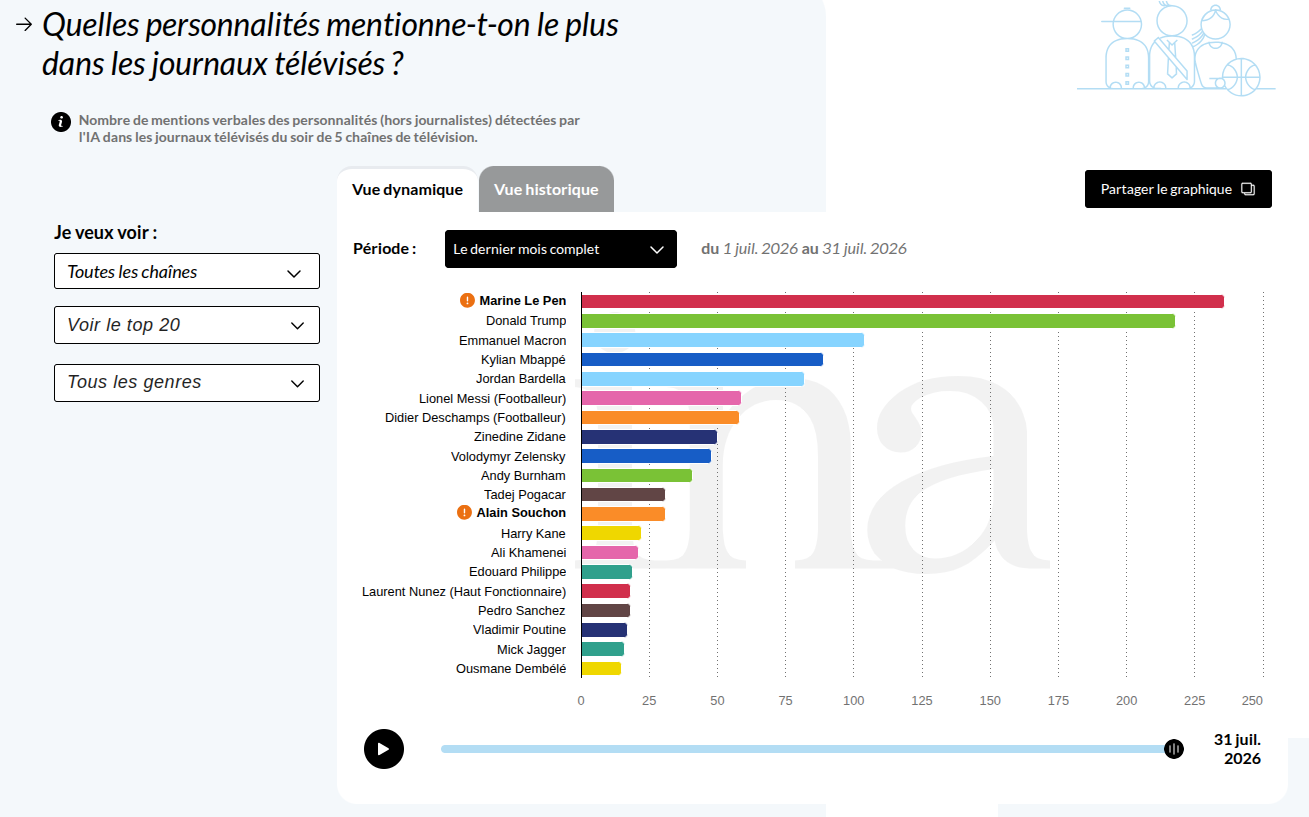
\includegraphics[width=1\linewidth]{./illustrations/dataina.png}
	\caption{Capture d'écran du site data.ina.fr du graphique des personnalités les plus mentionnées dans les journaux télévisés au cours du mois dernier (à la date du 09 septembre 2026).}
	\label{fig:dataina}
\end{figure}
L'existence de ce site manifeste l'aboutissement des travaux sur l'INA sur l'IA et la capacité qu'elle a à se soustraire à une analyse humaine. 

\subsection{l'IA et les documentalistes}

%% Point sur le rôle qu'ont les documentaliste dans l'implantation de l'IA à l'INA et leur avis sur le sujet %%

Si tous ces projets d'utilisation de l'IA ont pour objectif d'améliorer le traitement documentaire d'une façon ou d'une autre, ils ont également un impact sur le cœur même du métier de documentaliste. Si ce sont aux ingénieurs de penser et développer ces outils. C'est aux documentalistes de construire les prompts, de superviser l'apprentissage des outils, et vérifier le travail réalisé et de le corriger. C'est un sujet qui suscite beaucoup d'échanges entre documentalistes : entre la peur de voir disparaître l'essence de son métier et l'assurance de voir de plus en plus de fonds pouvant être décrit et indexé. Ces sentiments se retrouvent auprès des deux documentalistes interrogés. Sont remis en question notamment la légitimité à utiliser de plus en plus d'IA pour des questions de temps et d'argent quand cet outil entraîne également des coûts non négligeables ainsi que des interrogations d'ordre écologiques. Mais aussi le soulagement de ne plus avoir à traiter des sujets considérés ennuyant ou peu stimulants. 

Et d'un autre côté, sont toujours évoqués l'importance de l'expertise du documentaliste. Il ne semble pas y avoir de crainte pour le moment que l'Intelligence Artificielle soit capable de remplacer l'expertise et l’œil de ces documentalistes. Pour mettre en marche ces IA, la médiation humaine reste au centre de cette évolution. De plus notre documentaliste interrogée remet en cause sa fiabilité. Nous avons évoqué à plusieurs reprises que l'erreur humaine imprégnait le traitement documentaire, quel que soit l'institution patrimoniale mais elle est le plus souvent de l'ordre de l'omission ou de la faute de frappe. Ces erreurs mettent en péril leur repérabilité dans la base de données comme nous l'avions vu avec la notice d'\enquote{Images de Turquie} mais elles ne produisent pas de contre-sens comme le ferait une intelligence artificielle qui hallucine. La documentaliste cite dans ce cas une émission indexée par IA lors de tests qui faisait remonter le terme de terrorisme, jamais évoqué dans l'émission. Cette technologie est toujours en cours d'amélioration mais cela questionne la plus-value d'un outil dont les résultats nécessitent la vérification d'un documentaliste. Dans ce cas le gain de temps supposé est remis en question. 

D'autant plus que l'INA tient une posture de référent dans la conservation et communication d'archives audiovisuelles et qu'il n'est pas envisageable de garder des résumés provoquant des contresens pour l'utilisateur\footnote{(Opinions recueillit lors d'entretiens avec une documentaliste de l'INA, Pascal Lebeurier et Arthur Hénaff, voir la section \enquote{L'impact des nouvelles technologies - de l'IA} ~\ref{ann:transcriptions},\nameref{ann:transcriptions}), p.~\pageref{ann:transcriptions}. Pour plus d'informations sur l'impact de l'IA sur le métier de documentaliste le mémoire \enquote{Evolution du métier de documentaliste dans le contexte du déploiement de l'IA à l'INA} par Ghitta Mellah est à paraître.}. 

De la même façon que l'IA entre de plus en plus dans les habitudes de la société, certaines documentalistes ont également recours à l'IA dans leurs pratiques quotidiennes, en dehors des outils mis à leur disposition ou à tester. Des grands noms parmi les intelligences artificielles conversationnelles comme ChaptGPT, Copilot, Claude sont autant utilisées dans le développement des outils de l'INA que chez les documentalistes pour les accompagner dans leurs missions, en les aidant à rédiger, à se corriger etc... Ici aussi les avis divergent, notre documentaliste interrogée dit préférer rédiger en autonomie mais comprend que d'autres collègues puissent y avoir recours. 

\subsection{L'IA et l'accessibilité aux collections}

%% L'impact direct de l'IA dans le traitement documentaire actuellement (Hors documentalistes)%%

Des documentalistes interrogés, ce ne sont pas forcément toutes ces avancées de l'IA qui revenaient le plus mais plutôt la transcription automatique par IA qui utilise la reconnaissance de la parole et des outils d'indexation assistée\footcite[][150]{caporiondo-prost2026}. Cet outil est souligné comme étant une compensation au manque de description de certaines émissions du à la quantité massive de données, certaines typologies comme les fonds régionaux, longtemps négligés\footnote{(Voir entretien d'une documentaliste de l'INA sur l'impact de la politique documentaire sur les données de description ~\ref{ann:transcriptions},\nameref{ann:transcriptions}), p.~\pageref{ann:transcriptions}.}. Ils contribuent à compenser les différences de politique documentaire et de vocabulaire, notamment lors de l'indexation. Dans ce cas, Pascal Lebeurier nous cite une commande traitant du réchauffement climatique. En se fiant à l'indexation, le document le plus ancien était de 77 mais grâce aux transcriptions, les documentalistes ont pû faire ressortir un document de 1950 utilisant déjà le terme de \enquote{réchauffement climatique}. Encore une fois, les données descriptives décrivaient seulement une \enquote{expédition Groenland}. Les transcriptions viennent compléter les descriptions pré-existantes et parfois compenser leurs défauts et ainsi facilitent l'accès à toutes les collections. 

Mais aujourd'hui, et ce malgré le complément important que ces transcriptions apportent aux notices lacunaires, les transcriptions ne sont pas accessibles à tous les publics. C'est principalement les personnes internes à l'INA qui bénéficient de cette avancée et en écoulement, des personnes qui bénéficient des services de recherche de ces documentalistes comme les professionnels de l'audiovisuels. En effet, ces transcriptions ne sont pour le moment accessibles que sur l'outil de consultation Notilus, toujours en développement et inaccessible aux publics. Pourant la demande est forte, notamment au sein du Lab. Mais il est pleinement envisagé de mettre à disposition des publics ces transcriptions dans les outils en développement comme l'ont évoqué Pascal Lebeurier et Arthur Hénaff\footnote{(Voir transcription des entretiens~\ref{ann:transcriptions},\nameref{ann:transcriptions}), p.~\pageref{ann:transcriptions}.}. 

%% Conclusion %%

L'intégration des transcription par IA est une transformation importante des méthodes de recherche qui permettent de contrebalancer certaines difficultés à la recherche dans les bases de données dues à l'évolution des politique documentaires et à la massification des données. D'une autre part, cela impacte également la pratique du traitement documentaire, leur implication dans les outils d'intelligence artificielle suppose que les institutions ont une grande responsabilité dans la fiabilité des données, surtout pour des institutions comme l'INA ou la BNF qui ont une posture de référents dans leur domaine. Il est également sensé de questionner l'impact que cela aura sur le métier de documentaliste. Ce métier tiens une posture d'expert des collections mais il court de risque de glisser vers une statut de contrôleur des données générées par IA. Nous sommes au cœur d'une évolution majeure des politiques documentaires. Avec l'intelligence artificielle s'ouvre la possibilité d'améliorer l'accessibilité aux collections. Bien qu'elle vienne également avec son lot de nouvelles réflexions. Outre les interrogations sur l'impact écologiques et économiques de telles pratiques ainsi que sur la gouvernance des données, elles portent sur la place de l'expertise des documentalistes mais aussi sur la place à donner à des analyses réalisées par IA dans les notices descriptives. Questionnant au passage la posture de référence que tiennent ces institutions en terme de documentation si la description vient à être totalement automatisée. 
	
\chapter*{Conclusion de la partie 2}

%% Général %%

Dès leur création, les institutions patrimoniales font face à plusieurs facteurs d'influence sur leur traitement documentaire. Nous en avons soulevé les principaux concernant l'institut national de l'audiovisuel. Certains de ces facteurs ont affecté d'autres institutions, c'est particulièrement le cas des nouvelles technologies. Au fil des années, la documentation et le traitement documentaire se sont continuellement adaptés à ses évolutions, des balbutiements de l'informatique à l'avènement de l'intelligence artificielle. D'autres facteurs sont eux plus spécifiques à l'institution. Dans ce cas, la fragilité des supports conservés par l'INA ont motivé une campagne de numérisation exceptionnelle. D'un point de vue plus institutionnel, quand l'institut national de l'audiovisuel se voit confier le dépôt légal des diffusions télévisées, le traitement documentaire s'en voit affecter de diverses manières. De façon directe quand il faut adapter la description des documents à de nouveaux publics et de nouveaux usages mais aussi de façon indirecte. Quand il est affecté par la séparation des services patrimoniaux de l'institution pour séparer les archives professionnelles des diffusions du dépôt légal puis quand le budget impose une retenue dans la sélection des documents traités et le traitement qui leur consacré. 

%% INA - Première partie %%

Ainsi, si nous tentons de retracer les principales politiques documentaires et leurs perturbations nous commençons à la première cinémathèque de l'ORTF. La politique documentaire est à des fins commerciales, les documents sont traités en stocks et les informations que l'on y trouve servent les cinémathécaire de l'ORTF pour retrouver facilement des images d'illustrations pour les journaux télévisés. Les fiches correspondant à cette politique crées avant 1975 ont été reprises par des prestataires et vérifiées par des documentalistes dans les années 90. A partir de 1975, les premières bases de données font leur apparition. Dans un premier temps suivant la logique de bibliothèque puis s'adaptant aux nouvelles normes. Entre les deux bases de données, lors du versement, certains champs ne correspondant pas ont été versés de la première base à la deuxième. En 1992 la loi du dépôt légal est voté, la conservation et la communication patrimoniale à des fins scientifique s'inscrit dans les missions de l'INA. Tout en continuant sa conservation et communication à des fins commerciales, l'INA met en place une nouvelle politique documentaire appliquée au flux. Cette nouvelle politique est au service de ce nouveau public de chercheurs qui étudient autant les émissions que leur diffusion. Pour cela les professionnels de l'INA se séparent en deux services et utilisent outils de production et de consultations, appuyés sur différentes bases de données. Pour faire face à l’afflux massif de données, les professionnels de l'INA mettent en place différents types de traitements. C'est par ce prisme que le traitements documentaire est désormais affecté car une fois mis en place, ils ne changeront presque plus. Ce qui changera, c'est la question de programme, quel chaîne se voit assigner quel traitement. Pour répondre à cette question, de nombreux critères rentrent en compte : quelle quantité de données l'INA collecte-t-elle, combien en conserve-t-elle, quel temps son budget lui permet-il d'assigner à leur traitement. En 2020, les deux services patrimoniaux fusionnent mais les deux politiques documentaires persistent. Malgré une communication facilitées entre les responsables de fonds dévolus et non dévolus, les outils de production et de consultation restent résolument doubles. Et ce alors que le traitement documentaire continu d'évoluer face à l'intégration de l'IA dans les pratiques documentaires. 

%% Reprise d'antériorité %%

Et pour conclure, parmi toutes ces notices issues de politiques documentaires différentes, affectées par plusieurs facteurs internes ou externes à l'institution, certaines de ces notices anciennes ont potentiellement été l’œuvre de reprises d'antériorité, elles aussi effectuées, selon les politiques documentaire et les situations institutionnelles, technologiques et budgétaires en vigueur à leur époque, éliminant l'indexation utilisée à la création de la première, surtout pour les fiches papiers postérieures à 1975 dont nous n'avons plus de traces, au contraires des fiches papier précédent 1975. Tout cela alors que très peu de ces changements ne sont documentés. 

%% Technologies - Les solutions déjà mises en place %%

De plus, le traitement documentaire en vigueur n'est pas figé dans le marbre, il est en constante évolution, notamment avec l'utilisation de l'intelligence artificielle générative  qui permet d'améliorer l'accessibilité aux collections tout en remettant en question le métier de documentaliste. Il faut prévoir son impact sur le traitement documentaire.   

%% Ouverture à la partie qui suit %%

C'est avec toutes ces informations en tête que nous avons élaboré un outil ayant pour objectif de faciliter l'accessibilité aux collections de l'INA. Désormais nous avons conscience des enjeux que représentent l’accessibilité aux collections dans les institutions patrimoniales et plus particulièrement à l'INA ainsi que l'origine des de ces enjeux. Nous disposons de toutes les informations nécessaire pour construire un outil pouvant mettre à contribution les outils facilitant l'accès aux collections tout en offrant une solution pour tous les défauts résultant de l'évolution du traitement documentaire. 
		
\part{Conjuguer découvrabilité et recherche précise}

Notre préoccupation, lors de l'élaboration de ce projet de cartographie du traitement documentaire a donc été, non pas de proposer un outil pour l'exploration des collections étant donné qu'ils existent déjà et que de nouveaux outils sont développés, mais d'un outil proposant aux utilisateurs de nouvelles perspectives d'accessibilité aux bases de données qui permettent de contourner les contraintes d'accessibilité dues à l'évolution des politiques documentaires. Cet outil a été pensé en complémentarité aux outils de consultation des données, comme un outil améliorant l'accessibilité les collections afin de permettre aux utilisateurs de préparer leur recherches. 

Dans ce but, nous allons déjà présenter les outils dont nous disposons pour améliorer la découvrabilité des collections par le traitement documentaire. Puis nous conclurons notre propos en évoquant comment nous pouvons adapter le processus de recherche des utilisateurs de la base de données à ces enjeux d'accessibilité notamment en appuyant l'importance que nous avons porté à l'expérience utilisateur dans le cadre d'une recherche avec notre outil.  

	\chapter{Permettre la découvrabilité}
	
		\section{Cartographier les données}
		
		%% Parler de data.ina.fr : parce que nous aussi on permet d'avoir plusieurs clefs d'entrée etc... A la conclusion de toute fin dire que la réalisation du projet est incertain et dépend de l'aboutissement d'autres projet (comme Notilus et compagnie)
\subsection{La découvrabilité dans les institutions patrimoniales}

%% Introduction : Définition de la découvrabilité %%

La \enquote{découvrabilité}, dans l'environnement numérique, se définit comme la capacité à voir, accéder et consulter un contenu parmi un ensemble important d'autres contenus\footcite{decouvrabilite}. On le différencie de la repérabilité, qui définit la capacité à trouver un contenu en ligne, par son caractère non intentionnel. Un contenu est découvrable si un utilisateur peut s'y trouver confronté, sans que cela soit son intention première. Au cours des dernières années, cette notion a pris une grande importance pour les institutions patrimoniales, notamment lors du basculement de la consommation des contenus en ligne avec le confinement\footcite{decouvrabilite}. Cette notion s'applique en général au contenu sur le web mais ce n'est pas le cas dans ce projet. Précédemment, nous avons constaté que, grâce au web et aux réseaux sociaux, l'INA est aujourd'hui une institution de référence en matière d'archives audiovisuelles. Il est fort probable qu'une personne francophone, à la recherche de contenus audiovisuels d'archives finira par entrer en contact avec un site ou un réseau social de l'INA. Nous en avons nous-même fait l'expérience en tentant de nous mettre dans la peau de ce profil. Dans le contexte d'une recherche en ligne avec le moteur de recherche Google, le site de l'INA \enquote{ina.fr} est le premier résultat aux recherches \enquote{vidéos d'archives}, \enquote{archives audiovisuelles} et il apparaît dans la première page de résultat avec les recherches \enquote{Cinq colonnes à la une}, \enquote{anciennes émissions tv}, \enquote{début TF1}, \enquote{passage à la couleur tv france}. Dans le contexte des réseaux sociaux, il est plus difficile de déterminer la vitesse à laquelle nous pouvons rencontrer un contenu de l'INA ou de toute autre institution patrimoniale car le fonctionnement algorithmique des réseaux sociaux est très opaque et change régulièrement\footcite[252]{farchy2023}. Nous pouvons tout de même supposer que la production de parodies de documents diffusés par l'INA ou la production de fausses archives par intelligence artificielle génératives reproduisant les codes de ce même document sont tous deux des indicatifs de la forte présence de l'INA sur le web et les réseaux sociaux. 

Nous avons pu constater, au cours du développement de cet exposé, que la découvrabilité des contenus des institutions patrimoniales est une problématique au centre des stratégies de communications de ces institutions, y compris l'INA. C'est pourquoi l'outil que nous souhaitons mettre en place n'a pas pour objectif d'améliorer la découvrabilité des collections de l'INA sur le web mais plutôt la découvrabilité de tous ses documents dans ses bases de données. Actuellement, la principale méthode d'utilisation des bases de données de l'INA est de savoir ce que l'on recherche tout en possédant une connaissance des changements de politiques documentaires s'appliquant aux périodes qui nous intéressent. La découvrabilité est restreinte car l'outil de consultation Hyperbase n'a pas été pensé dans un objectif de découvrabilité mais de recherche.

\subsection{Cartographier les données}
%% Définition de datavisualisation %%

Le premier outil auquel nous avons eu recours pour faciliter l'accessibilité aux collections est la datavisualisation. Elle permet de mobiliser une quantité massive de données afin d'en faire ressortir des informations plus accessibles à l'échelle de l'utilisateur. Grâce à cet outil, il est possible de faire correspondre une quantité importante de données à des structures graphiques\footcite[][42]{fourlinnie2016} permettant à un utilisateur ne connaissant pas ces bases de données de comprendre ce qu'elles contiennent et ce qu'il peut y trouver. Face aux données massives que représentent les collections numériques de l'INA, c'est un outil qui est précieux. Par l'utilisation de formes graphiques, nous pouvons simplifier la complexité des bases de données de l'institut. 

%% Premier type d'utilisation : Vision globale des données de toute la collection %%

Parmi les différentes manières de représenter nos données, la première, et celle qui semble la plus évidente, est de réaliser une visualisation de l'ensemble des collections. C'est ce qu'a fait le laboratoire de recherche de la bibliothèque publique de New-York (NYPL Labs) en réalisant une projection graphique de leurs collections. Ils ont rapproché les différents sujets indexés dans leur collections selon le nombre d’occurrence de ceux-ci dans les ouvrages de leurs collections. Plus un terme d'indexation apparaît, plus la \enquote{bulle} qui lui associée est grosse.

\begin{figure}[H]
	\centering
	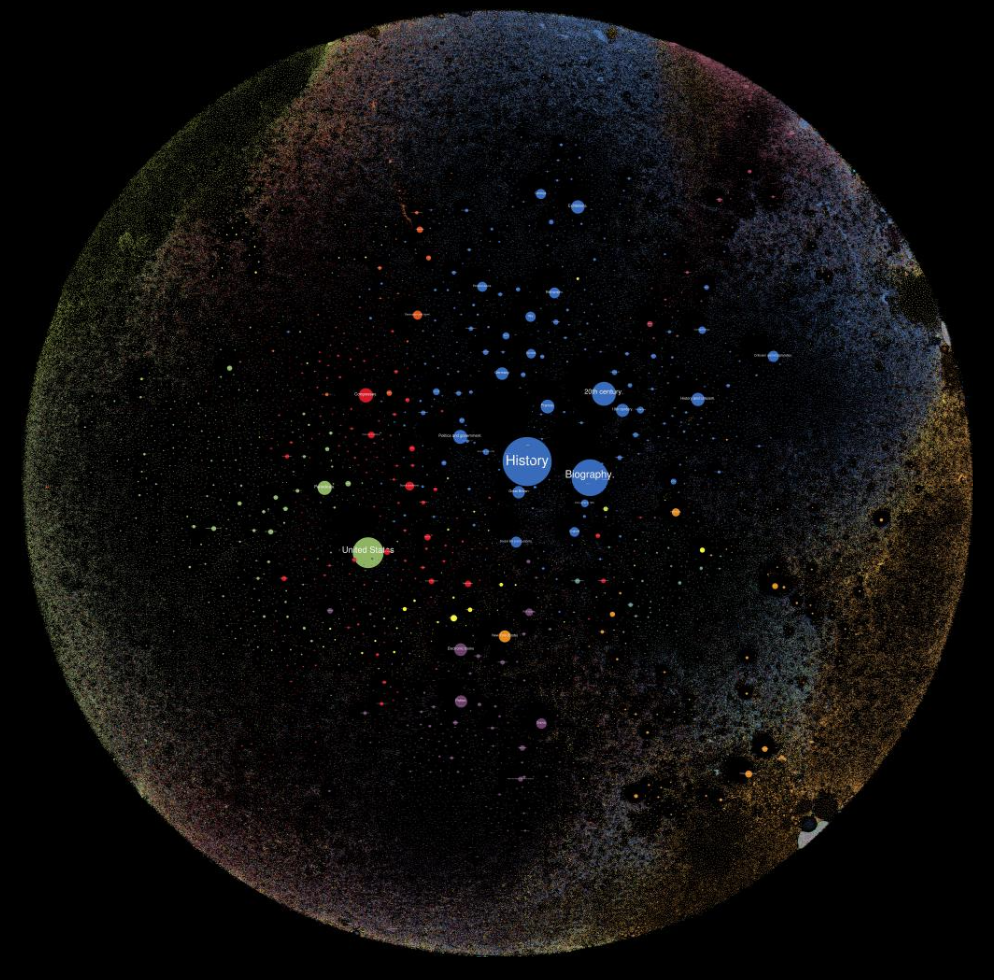
\includegraphics[width=0.70\linewidth]{./illustrations/NYPL_graph.png}
	\caption{Capture d'écran du graphique de la NYPL Lab}
	\label{fig:NYPL_graph}
\end{figure}

%% Application à l'INA %%

Cet exemple nous permet de questionner les données à choisir lors de la conception d'une visualisation de données : quelles informations à quels questions cette visualisation doit-elle répondre ? Selon l'angle que nous abordons dans ce mémoire, il n'est pas pertinent de faire ressortir les données d'indexation des collections comme l'exemple cité précédemment car notre outil est concentré sur la compréhension du traitement documentaire des collections. Faire ressortir les données d'indexation ne ferait qu'accentuer le manque de visibilité des collections n'étant pas indexées. Pire, car nous pouvons toujours utiliser cette visualisation pour mettre en avant les documents non indexés, ce qui en un sens illustrerait une histoire de l'institution que nous avons déjà précédemment décrit. Mais quid des documents indexés avec des termes désuets qui disparaîtraient totalement dans la masse, ce qui irait à l'encontre de cette volonté d'utiliser les datavisualisations pour accompagner l'utilisateur dans l'exploration de ces collections avec un traitement documentaire inégal. Notre objectif est de faire ressortir la richesse de notre base de données, pas d'accentuer ses défauts. Dans le cadre de l'utilisation de datavisualisations au service de la découvrabilité des collections, nous souhaitons utiliser ce premier type de datavisualisations afin d'introduire l'utilisateur aux différences de traitement documentaire qui se présenterons lors de son exploration de la base de données. C'est pourquoi, nous avons fait le choix de présenter aux utilisateurs, sur la première page de notre outil, une visualisation en bulles groupées de l'ensemble des collections\footnote{Toutes les visualisations de données ont été réalisées sur Tableau Public avec une extraction de la base de données du dépôt légal DLTV contenant toutes les émissions en première diffusion de la chaîne France 2 et Arte, voir Annexe \ref{ann:cdc},\nameref{ann:cdc}), p.~\pageref{ann:cdc}.}. 

\begin{figure}[H]
	\centering
	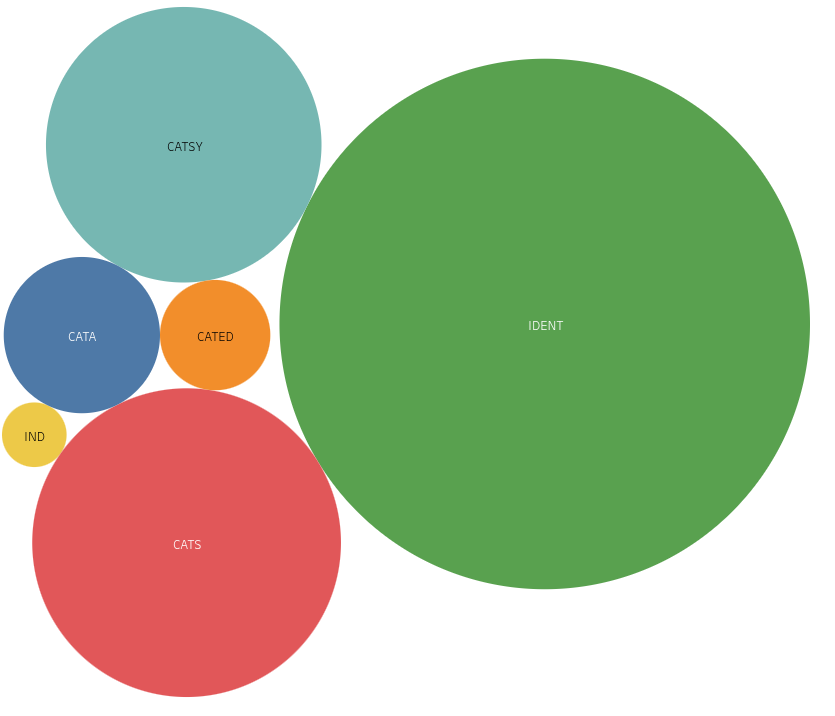
\includegraphics[width=0.75\linewidth]{./illustrations/graph_ina_tout.png}
	\caption{Graphique en bulles groupées du traitement documentaire dans les bases de données de l'INA}
	\label{fig:graph_ina1}
\end{figure}

Ce graphique permet à l'utilisateur de faire une première entrée dans la base de données et d'en comprendre la composition. Il a la double fonction d'introduire l'utilisateur aux informations qu'il peut trouver dans la base de données et de servir d'illustration à un texte expliquant les différents traitements appliqués aux documents, dans une version bien plus simplifiée, semblable aux connaissances que dispenseraient les documentalistes de l'INAthèque. Cela dit, grâce à cette visualisation, l'utilisateur comprend que les données qu'il va exploiter n'ont pas un traitement égal, mais cela ne suffit pas à permettre la découverte des collections. Tout au long de ce mémoire, nous avons à de multiples reprises appuyé sur le fait que ce manque d'accessibilité aux données étaient dues à un enchaînement de politique documentaire. En conséquent, il est important de prendre en considération les données temporelles dans nos datavisualisations. 

%% Image d'un phénomène non perceptible visuellement %%

Pour cela, une vue chronologiques des données permet de démontrer l'évolution de ces pratiques documentaires. C'est l'idée qui est mise en avant par la représentation chronologique de l'entrée des données des arbres et plantes conservées dans l'aboretum de Harvard\footcite{loukissas}. Cette base de données est également marquée par des changements de politiques documentaires, dans ce cas ce sont les numéros d'accessions dont la logique d'élaboration a été affectée par différentes politiques documentaires. Cette visualisation permet de mettre en avant l'activité d'indexation dans le temps.

%% Application à l'INA %% 

Cette visualisation est plus pertinente dans notre démarche de médiation du traitement documentaire de collections patrimoniales. Elle permet à l'utilisateur de ces bases de données de comprendre en un coup d’œil la situation des collections qu'il consulte et aviser ses pratiques en conséquence. Il peut se diriger vers le traitement qui contiendra les données qu'il recherche ou adapter sa recherche aux champs que comprennent les notices qu'il désire. En adoptant une approche temporelle, cette visualisation est particulièrement adaptée à une étude historiques. La visualisation qui suit a été crée avec l'outil \enquote{Tableau Public}, d'après une extraction de toutes les notices d'émissions en première diffusion de la chaîne France 2 sur la base de données du dépôt légal.

\begin{figure}[H]
	\centering
	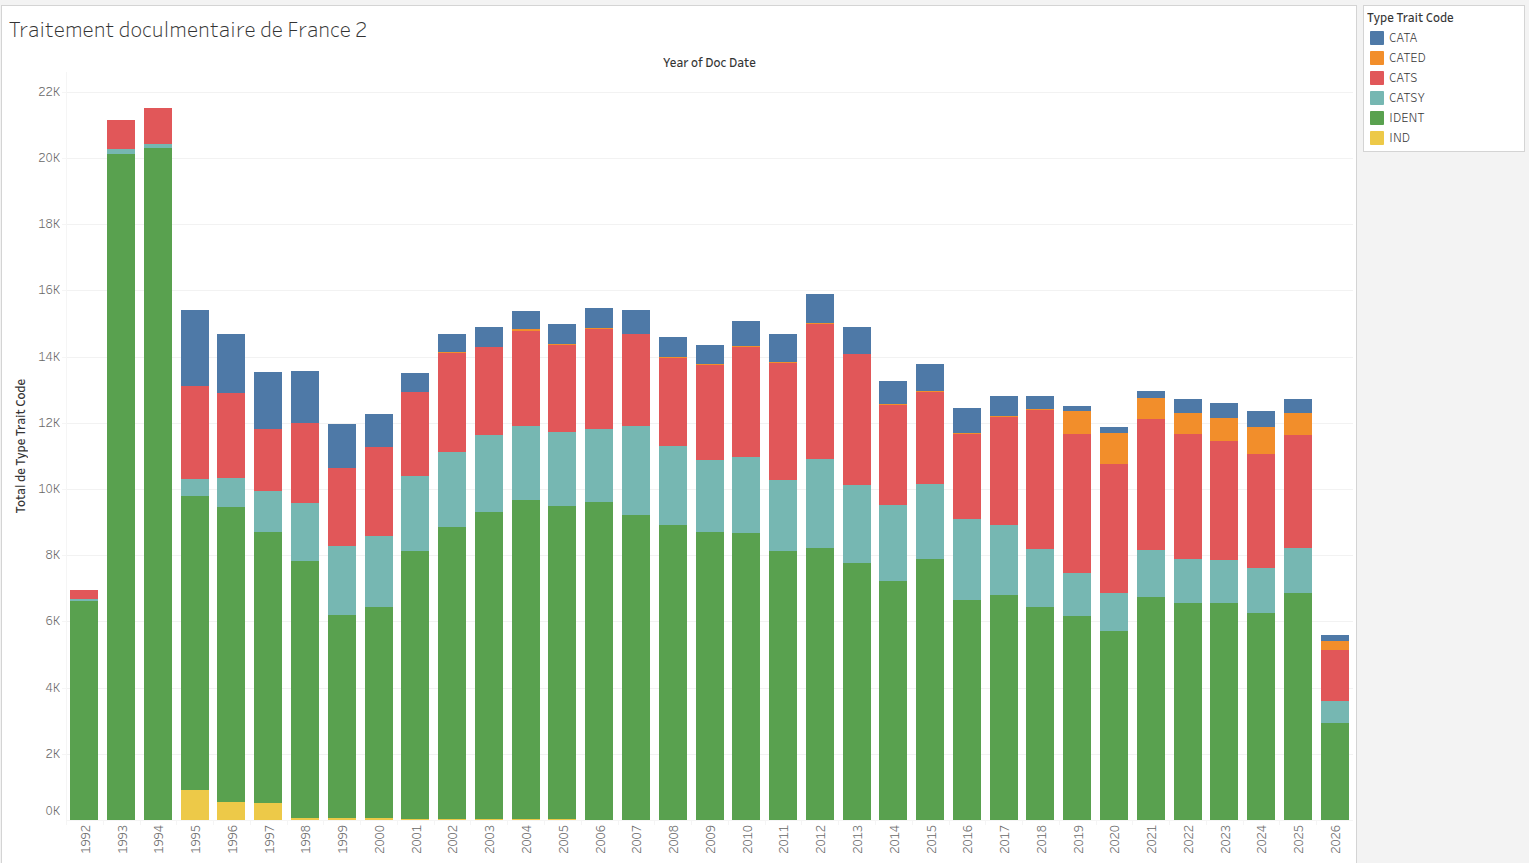
\includegraphics[width=1\linewidth]{./illustrations/traitement_FR2.png}
	\caption{Visualisation du traitement documentaire chronologique de la chaine \enquote{France 2}}
	\label{fig:traitement_FR2}
\end{figure}

Dans ce graphique en barre réalisé sur les données de la chaîne télévisée France 2, l'utilisateur peut récupérer en quelques instants les informations dont il peut avoir besoin. Sur l'axe des ordonnées s'affiche le nombre de notices et sur l'axe des abscisses les années. Grâce à ce graphique, l'utilisateur peut donc savoir le nombre d'émissions traitées chaque année ainsi que le traitement le plus utilisé, à la fois pour chaque année mais aussi sur l'ensemble de la période durant laquelle cette chaîne a été traité. Grâce à ces informations, tirées des données des bases de l'INA et mis en forme grâce à ce graphique l'utilisateur a une vue générale sur le traitement documentaire de cette chaîne et peut donc orienter ses recherches sur la période durant lesquelles le traitement correspond aux informations qu'il recherche ou au contraire, si il a déjà effectué une recherche sur cette chaîne, sans succès, il peut comprendre pourquoi. Le présent exemple fonctionne sur une chaîne mais également sur un programme isolé ou même sur un genre.

\begin{figure}[H]
	\centering
	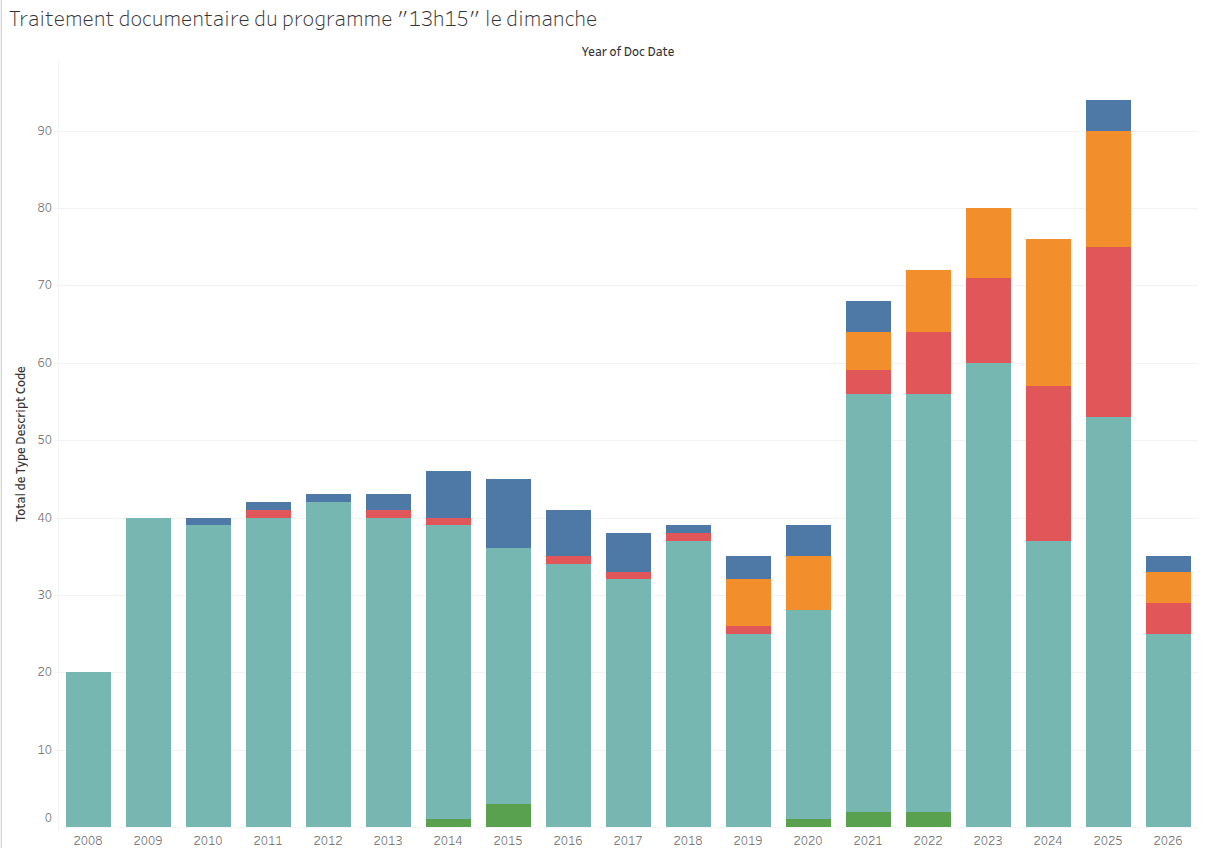
\includegraphics[width=0.75\linewidth]{./illustrations/graph_ina_programme.png}
	\caption{Visualisation du traitement documentaire chronologique du programme \enquote{13h15 le dimanche}}
	\label{fig:traitement_13h15}
\end{figure}

\begin{figure}[H]
	\centering
	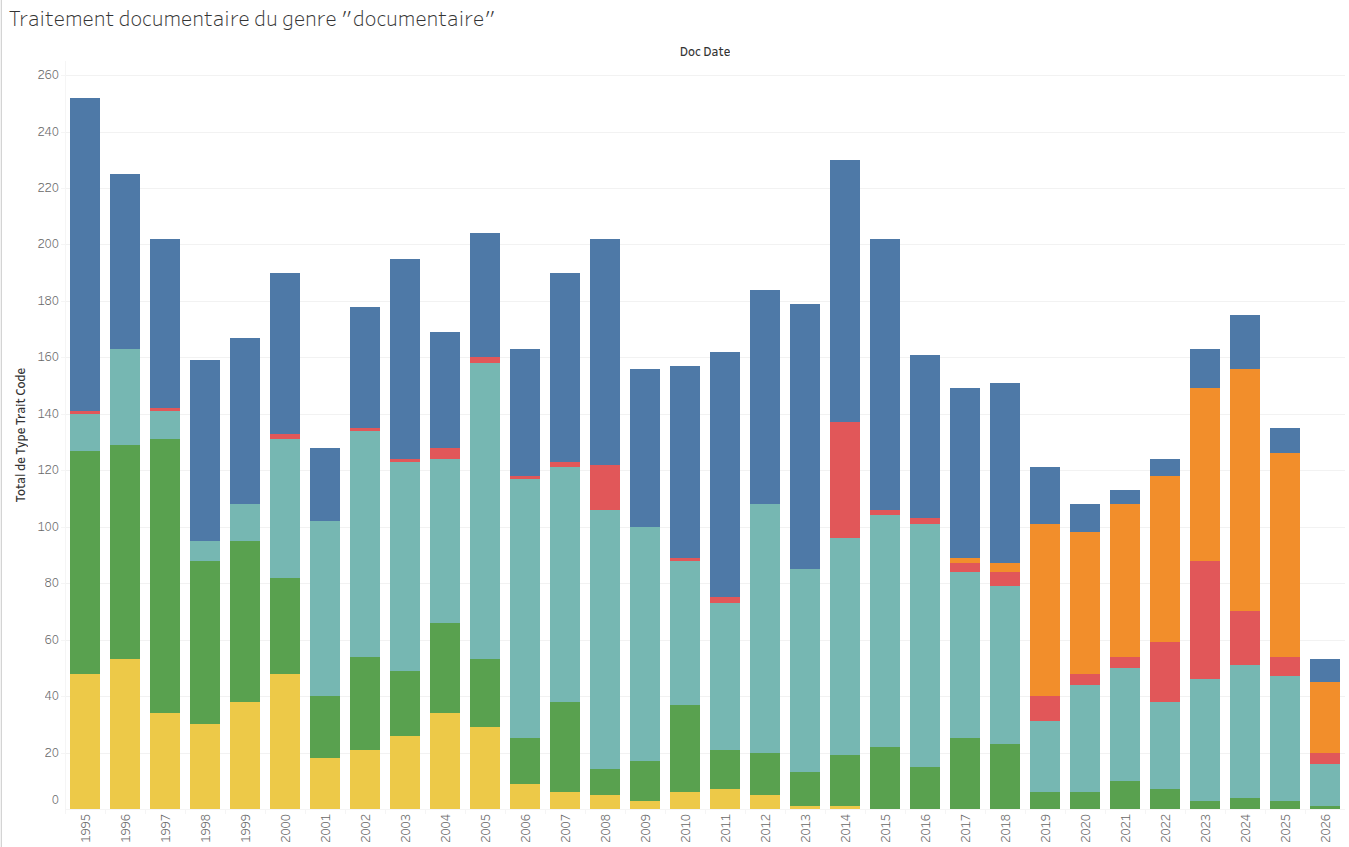
\includegraphics[width=0.75\linewidth]{./illustrations/graph_ina_genre.png}
	\caption{Visualisation du traitement documentaire chronologique du genre \enquote{documentaire}}
		\label{fig:traitement_docu}
	\end{figure}
	
En mettant à disposition toutes ces datavisualisation, mettant à contribution les données des dates de diffusions et du type de traitement appliqué, nous parvenons à donner aux utilisateurs trois différentes portes d'entrée dans les données. 

%% Utilisation de l'INA pour la découvrabilité : data.ina.fr : Montrer que c'est courant d'utiliser les datavisualisations pour améliorer la découvrabilité des données %%
		
		\section{Expliquer les données}
		
		%% Correction des données %%

Ces visualisations peuvent également contribuer à mettre en avant les irrégularités des bases de données. Dans le cas de l'INA, nous avons soulevé que certaines politiques documentaires ne circulaient qu'à l'oral ou par mails, ce qui signifie que nous ne pouvons pas les suivre. Grâce à la visualisation de ces collections, nous pouvons cibler ces irrégularités, comprendre pourquoi elles existent et mettre en place une médiation pour permettre aux utilisateurs d'accéder à ces données ou même les corriger. Il semble moins insurmontable de cibler des erreurs qui sont ostensiblement visibles plutôt que d'aller rechercher la trace de chaque petit changement de \gls{pd} dans des milliers de mails. Lors de la réalisation de tests de visualisation du \gls{td} chronologique de la chaîne \enquote{France 2}, nous avons notamment relevé des erreurs se prêtant à ce cas. La chronologie commence en 1992 parce c'est la date de création de la chaîne sous le nom \enquote{France 2}. Ce qui nous interpelle, c'est qu'avant 1995, date à laquelle le dépôt légal a été mis en place à l'INA, il y a un nombre plus important de notices, plus que toutes les autres années et toutes les notices sont en IDENT (Identification), donc sans aucun \gls{td}. Cela force la réflexion sur ce sujet. 
%REDEMANDER EXPLICATION. 

%% Attention aux biais %%

%% Les biais sont très courants dans les datavisualisations. On peut faire dire n'importe quoi à des images, en l'occurence des graphiques. C'est pourquoi il est important que les documentalistes restent impliqués dès le départ. 

%% Conclusion de la sous-partie 2 : %%

Cela dit il est important de souligner que cet outil a été pensé pour les bases de données du dépôt légal. Il n'est pas possible de faire des recherches dans les champs utilisés par le dépôt légal. De la même façon qu'il tente de régler des problèmes qui ont sans doute été réglés par les nouveaux outils à venir. Certains problèmes soulignés ont déjà été étudiés et corrigés par le service qualité de l'INA. Mais ces corrections concernent principalement la qualité des données. L'avantage de cet outil et plus précisément des datavisualisations est qu'il a été adapté pour correspondre à différentes bases de données. Ainsi, il est possible de l'utiliser sur d'autres bases, comme le lac de données car les enjeux d'accessibilité aux collections dues à cet enchaînement de politiques documentaires est propre à ces collections. Cet outil reste pertinent pour d'autres bases de données plus adaptées aux nouveaux modes de consommation des données, sans perdre de sa pertinence, même si il nécessite d'être adapté en conséquence. 

%% Conclusion du chapitre :%%

Cela dit, nous ne devons pas négliger que cet outil est à destination de personnes ayant pour objectif d'utiliser les bases de données de l'INA et plus précisément du dépôt légal. L'utilisateur peut rencontrer de nouveaux contenus par hasard, mais il reste important d'avoir une idée de départ de ce qu'il recherche : une chaîne, une genre etc... En partant d'une des clefs d'entrée de notre outil peut découvrir des documents qu'il n'aurait jamais rencontré involontairement lors d'une recherche sur Hyperbase mais il ne peut pas partir de vraiment rien. Cet outil a avant tout été imaginé en appui à la recherche, de ce fait, c'est la fonctionnalité à laquelle nous avons prêter le plus d'attention. 
		
	\chapter{Permettre la recherche}
	
	\section{L'expérience utilisateur}
	
	%% Introduction %%

L'objectif premier, lors de la création d'un outil, est qu'il soit utilisé par le public visé. Il n'y a pas d'intérêt à créer un outil si l'utilisateur ne le trouve pas assez attractif et avantageux pour l'intégrer à ses habitudes. Étant donné que nous souhaitons ajouter cet outil à la grande palette d'outils des utilisateurs des collections, nous avons particulièrement d'intérêt à prêter attention à l'expérience de l'utilisateur. 

%% Définition expérience utilisateur %%

Le terme d'\enquote{expérience utilisateur} est utilisé pour désigner les interactions d'un utilisateur avec un outil numérique. Une expérience utilisateur réussie assure que cet outil offre une expérience suffisamment agréable pour que l'utilisateur revienne plus tard à l'utilisation de cet outil ou qu'il rentre dans ses habitudes. De cette façon, les fonctionnalités doivent être suffisamment accessibles, pertinentes et performantes pour ancrer cet outil dans les habitudes des différents utilisateurs\footcite{silberstein2024} des bases de données des institutions patrimoniales. Cela ne passe pas forcément par le design mais plutôt les interactions de l'utilisateur avec l'outil. Elles doivent être agréables et lui fournir le résultat qu'il attend. 

\subsection{Garder l'attention de l'utilisateur et lui donner envie de revenir}

%% Application expérience utilisateur dans notre outil %%

Appliqué à notre outil, notre objectif est d'offrir la meilleure expérience possible avec notre outil, quel que soit son objectif en commençant à l'utiliser. Ainsi, si il n'a pas de recherche précise ou qu'il en cherche une et qu'il utilise, en conséquent cet outil dans une posture de découvrabilité des collections. Il doit disposer de plusieurs clefs d'entrée dans nos collections sans que l'expérience soit étouffante à cause de la quantité massive de données. Il doit pouvoir naviguer d'un contenu à l'autre sans se sentir perdu dans la structure des bases de données. Et surtout il doit pouvoir comprendre quelles informations il trouvera sur ces documents et pourquoi sans avoir à apprendre l'entièreté du fonctionnement des politiques documentaires à l'INA. Dans un autre sens, si il utilise cet outil avec une idée de recherche précise. Il doit pouvoir réaliser précisément la recherche qu'il souhaite sans que ni la qualité des données, ni le \gls{td} appliqué ne l'empêche d'accéder à tous les documents qui correspondent à sa recherche. Le résultat est clair, il ne se retrouve pas étouffé sous une quantité de données massives, il peut affiner sa recherche autant qu'il le souhaite puis sélectionner les notices qui l'intéresse et les sauvegarder pour pouvoir les rechercher sur les outils de consultation à sa disposition. La navigation entre ces différentes fonctionnalités est fluide, il ne perd pas de temps à chercher ce qui l'intéresse afin de ne pas le frustrer et le voir quitter l'outil. 

Afin d'atteindre cet objectif, nous nous sommes principalement concentrés sur la structure que mettra en place cet outil. Tout part de la page d'accueil sur laquelle sont développés les différents types de traitement appliqués par l'INA à ses documents. Nous dispensons ainsi une médiation sur le \gls{td}, par un.e documentaliste, contribuant à la fois au partage et à la conservation de ses connaissances. Cette explication est illustrée par la datavisualisation démontrant le type de \gls{td} majoritaire dans toute la base de données. De cette façon, cette illustration est la représentation graphique de ce qui est expliqué. A partir de cette page l'utilisateur a accès à deux onglets, l'un pour accéder à la recherche par chaîne, l'autre pour la recherche par programme. Ces deux onglets mènent tous deux à une page avec un moteur de recherche et des filtres pour affiner leur recherche. La seule différence entre les deux étant que pour la recherche par chaîne, toutes les chaînes sont déjà affichée en résultat. Pour la page des programme, nous avons estimé que cela serait trop lourd de charger toutes les émissions des bases de données et que cela serait trop envahissant pour l'utilisateur. Les résultats d'une recherche s'affichent sous la forme d'un tableau affichant un titre, les dates de diffusion, un résumé et un diagramme en secteur représentant la proportion de chaque traitement sur ce programme ou cette chaîne. 

\begin{figure}[H]
	\centering
	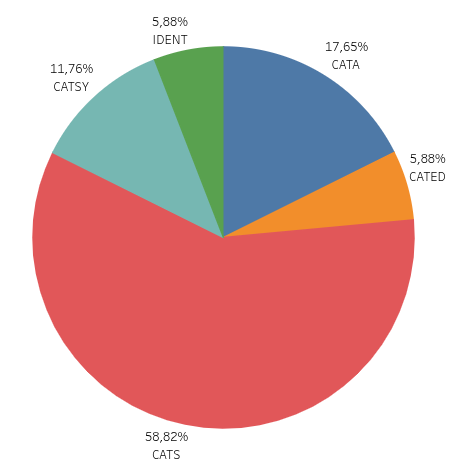
\includegraphics[width=0.5\linewidth]{./illustrations/graph_FR2_2.png}
	\caption{Visualisation par secteur du \gls{td} de la collection \enquote{13h15 l'après-midi}}
	\label{fig:traitement_secteur}
\end{figure}

En cliquant sur un résultat, une fiche s'affiche dispensant certaines informations sur la chaîne ou l'émission permettant de les situer dans le temps. Tout cela accompagné bien des graphiques en barre, représentés dans le \hyperref[fig:traitement_FR2]{chapitre précédent}. Ces graphiques sont personnalisables selon l'information que l'utilisateur recherche, en définissant des dates extrêmes pour les deux typologies (chaîne et émission) et en ajoutant des filtres pour choisir le genre pour la fiche chaîne. Auquel se rajoute le graphique de \gls{td} des genres sur cette chaîne. Avec cette structure, les utilisateurs suivent un cheminement simple, il y a peu de pages, toutes visibles dès la page d'accueil avec une organisation comportant strictement les informations dont les utilisateurs ont besoin pour construire le corpus dont ils ont besoin : identification du document ou de la collection et traitement appliqué, selon leurs critères personnalisés. 

\subsection{Garantir la lisibilité des informations : les datavisualisations}

Pour correspondre à l'expérience que nous souhaitons offrir, la notion de \gls{td} ne doit pas repousser l'utilisateur. C'est pourquoi nous avons fait appel aux datavisualisations. La représentation graphique simplifie visuellement l'information et en gardant le même code couleur pour chaque type de traitement sur l'ensemble de l'outil, les informations concernant le \gls{td} est plus facilement intégrable et l'ensemble des résultats et notices répondant aux mêmes codes visuels, l'utilisateur peut mobiliser rapidement l'information. 

%% Conclusion %%

Une des manières dont nous avons choisi de concrétiser cette expérience utilisateur favorable est l'utilisation des filtres afin de permettre à l'utilisateur de personnaliser au maximum sa recherche. 
	
	\section{Personnaliser la recherche}
	
	Toujours pour garantir cette expérience utilisateur, il est nécessaire d'ouvrir la recherche à plusieurs clefs d'exploration des données, de ne pas restreindre la recherche et anticiper les recherches des utilisateurs. Pour ce faire, l'utilisation des filtres prend une grand importance. Ils permettent d'éviter le phénomène de \enquote{surabondance de choix} généré par une quantité massive de données. Ce phénomène paralyse l'utilisateur dans ses choix\footcite[242]{farchy2023}, ou dans notre cas créer une \enquote{fatigue muséale} qui appliquée au numérique peut être identifié comme une fatigue mentale devant une quantité massive de données apportant plus d'informations qu'il n'est impossible d'appréhender\footcite[Notion développée dans :][5]{griveau2024}, ce qui est l'opposé de ce que nous souhaitons faire ici. Pour faciliter la recherche, nous avons divisé les filtres appliqués en deux.  

\subsection{Filtres de \gls{td}}

Premièrement, les utilisateurs disposent en page d'accueil d'une médiation du \gls{td} à l'INA, mais il est contre-productif de construire notre outil en partant du principe que ces informations seront lus, comprises et retenus par les utilisateurs. Cela sera le cas pour les documentalistes, mais pour un chercheur il serait frustrant de ne pas pouvoir accéder aux fonctionnalités de cet outil uniquement par l'apprentissage de notions assez précises de la documentation. L'expérience utilisateur serait compromises car le chercheur pourrait être réticent à intégrer cet outil à ses habitudes. Nous avons donc opté par l'adoption d'une recherche par filtre. Pour que les utilisateurs n'aient pas à retenir quel traitement contient quelles champs, nous avons établi qu'ils pourraient, en remplacement, sélectionner les informations qu'ils souhaitent trouver parmi : 
\begin{itemize}
	\item Descripteurs/mots-clés
	\item Chapeau : le terme étant un peu trop opaque pour un externe à l'INA, ce choix sera remplacé par description des images diffusées
	\item Résumé par séquence
	\item Liste de tous les intervenants
	\item Description plan par plan
\end{itemize}
Ces filtres correspondent aux champs trouvés dans les différents types de \gls{td}. Les résultats fourniront en conséquence les notices pour lesquels ces champs contiennent des données sans qu'il n'ait à intégrer que cela correspond à tel type de notices. 

\subsection{Filtres de documents}

Il sera également possible de réaliser cette recherche grâce à une barre de recherche qui cherchera la chaîne de caractère demandée dans le titre du document, de sa collection (dans ce cas, le terme de collection désigne le champs de la notice qui correspond au nom de la \enquote{série} au sein desquels il y a plusieurs \enquote{épisodes}) ou de sa tranche horaire. Nous avons en effet réduit les résultats à ces typologies de notices car chercher un résultat plus précis généreraient beaucoup de bruit et ne serait pas pertinent pour notre outil. Il ne sert à rien d'utiliser un outil tiers pour chercher une information que l'on retrouve déjà dans l'outil de consultation \enquote{Hyperbase}, notre objectif est de rassembler plusieurs données pour en faire ressortir des informations, pas d'afficher les mêmes informations mais sur un outil différent. 

Mais comme nous souhaitons offrir plusieurs clefs d'entrée dans nos données, sans restreindre la recherche, nous offrons également la possibilité de rechercher un contenu par l'utilisation de filtre. Les chercheurs n'ont pas toujours un titre d'émission précis en tête. De cette façon, si les filtres que nous avons décrit précédemment déterminaient quels champs l'utilisateur souhaitait voir, cette catégorie de filtre permet de choisir ce que les champs donnés doivent (ou peuvent selon leur choix) contenir. Quand les possibilités ne sont pas trop nombreux, le choix se fait par l'intermédiaire d'un menu déroulant affichant les champs possibles. Par exemple, pour la recherche par chaîne les filtres peuvent être entre autres : 
\begin{itemize}
	\item mode de transmission\footnote{A noter que dans ce cas cette information l'information recherchée n'est pas un champs mais plutôt quelle base de données interroger étant que les bases de données du dépôt légal sont divisés en chaîne hertziennes et satellites}. 
	\item Dates de diffusions : date de début, date de fin ou les deux.
\end{itemize}
Et pour les programmes : 
\begin{itemize}
	\item Genre : documentaire, journal télévisé...
	\item Chaîne de diffusion, de production 
	\item dates de diffusions
\end{itemize}
Cet outil doit libérer l'utilisateur du choix d'avoir à demander une chaîne de caractères précises dans un champs précis. Il est libre de savoir exactement ce qu'il recherche, comme en avoir une vague idée et de préciser ou agrandir sa demande en fonction des résultats. 
	
	\section{Situer un nouvel outil dans une structure institutionnelle et technologique en pleine transition documentaire}
	
	%% Introduction %%

Cela dit, le gros bémol que cet outil présente est la difficulté à le situer dans le temps. Pour le moment, cet outil figure parmi les projets du département de la direction des patrimoines. Son développement ne prendra place qu'à la direction Data \& Technologies dans une temporalité que nous ignorons. Il devient alors difficile d'évaluer quand débutera son développement et en conséquent de quels outils actuellement en développement, réflexion et en tests les utilisateurs des collections de l'INA disposeront-ils ? Les besoins peuvent varier si par exemple les chercheurs et professionnels de l'audiovisuel disposent des transcriptions des émissions ou encore de si les résumés par IA ont pleinement intégrés les bases de données. 

\subsection{Une question de base de données}

Le point sur lequel l'outil peut particulièrement varier est la base de données dans laquelle cet outil ira récupérer ses données. En l'état actuel, il a été pensé et construit sur l'exploitation des bases de données du dépôt légal. Si le lac de données vient à être en place pour plusieurs des publics visés, les défauts de qualités des données peuvent avoir été corrigés par cette nouvelle base de données. Il sera nécessaire d'adapter les datavisualisation pour le nouveau modèle de données. Les informations récupérées ne seront plus exactement les mêmes. Nous avions par exemple imaginés faire appel à wikidata afin de faire apparaître quelle chaîne succédait à quelle chaîne, sous quel nom. Ce que la base de données du dépôt légal ne permettait pas de faire mais que le nouveau modèle de données permettrait. 

D'un autre côté, il est pour le moment difficile de se projeter dans le lac de données car pour le moment, les données du dépôt légal ne sont pas intégrés à cet outil, mais seulement ses référentiels. 

\subsection{Manque de pertinence pour tous les publics}

Cet outil manque de pertinence pour les professionnels de l’audiovisuel qui seront confronté avec cet outil à des documents sur lesquels l'INA n'a aucun droit d'exploitation sans que ces indications ne paraissent dans les fiches créées par cet outil. Par nature, cet outil est conçu pour comprendre et suivre le traitement documentaire du dépôt légal. Les recherches sont effectuée par le titre de l'émission, de sa collection ou de sa tranche horaire. Ses fonctionnalités de correspondent pas aux besoins de professionnels de l'audiovisuel. Ces derniers vont donc continuer à se reposer sur les documentalistes. 

%% Conclusion %%

C'est pourquoi cet outil a été pensé pour s'adapter à toutes les évolutions possibles. Les datavisualisations ont été conçu pour montrer certaines informations. Le nom que prend les champs affichés et le modèle de données que suit la base de données ne sont pas de la plus grand importance. Nous avons conçu un outil fait pour fournir un service. Il est conçu pour le faire et s'adapter, peut importe les changements. 
	
\chapter*{Conclusion de la partie 3}

L'outil auquel nous avons réfléchi permet donc aux utilisateurs de se préparer en amont de leurs recherches avec les outils de consultation. Cet outil leur permet de comprendre et de voir la structure des bases de données du point de vue du \gls{td}. De cette façon, il leur est plus rapide de trouver les notices des documents contenant les informations qu'ils désirent. Ils peuvent réunir des corpus de document qu'ils désirent consulter en sachant exactement quelles informations il y trouvera. De cette façon, les utilisateurs de cet outil sont moins dépendants à la fois des connaissances des documentalistes et des outils vieillissants de l'INAthèque ne correspondant plus aux modes de consultations actuels. 

\chapter*{Conclusion}

Les enjeux que présente l'accessibilité aux collections des institutions patrimoniales ont donc trait à notre capacité à avoir accès à l'ensemble des collections, sans avoir connaissance des pratiques documentaires utilisées. En l'état actuel, il est difficile d'avoir une utilisation autonome des collections sans avoir de connaissances sur l'histoire du traitement des collections. Nous avons identifié les raisons de ce manque de visibilité sur l'ensemble des collections comme étant à la fois un mélange de plusieurs politiques documentaires facilement identifiables comme des périodes clés dans l'histoire de l'institution, une accumulation de changements mineurs non documentés et une adaptation des pratiques de traitement documentaire à l'informatisation des pratiques documentaires. Il en résulte une accessibilité qui repose principalement sur la transmission orale des connaissances approfondies des documentalistes. Afin d'offrir une meilleure accessibilité de ces documents, nous avons proposé la conception d'un outil d'appui aux outils de consultation des bases de données, proposant une cartographie du traitement documentaire des collections afin de fournir à l'utilisateur une représentation graphique compréhensible des données qu'il exploite, ainsi qu'une plateforme à même d'accueillir et de conserver les connaissances des documentalistes.

Cela dit, nous avons également constaté, tout au long de cette analyse, que certains outils sont en cours de développement. Ces outils offrent des solutions aux défauts des bases de données. Le lac de données, notamment, a effectué un travail important sur la qualité des données lors de la migration des bases de deux services patrimoniaux de l'INA. De plus, si nous avons constaté l'impact de l'enchaînement de différentes politiques documentaires, force est de constater que l'utilisation de l'intelligence artificielle est en passe de devenir la prochaine évolution des politiques documentaires. Seul l'avenir ne peut nous dire si cette nouvelle évolution sera avantageuse pour l'accessibilité aux collections ou si, au contraire, le bruit que provoquera ces données générées n'accentuent la confusion. 
	\addcontentsline{toc}{chapter}{Conclusion}
\newpage{\pagestyle{empty}\cleardoublepage}
	

%%%%%%%%%%%%%%%%%%

\appendix %Des appendices: tables figures, etc

% 1. Ajouter "Annexes" dans le sommaire
\phantomsection
\addcontentsline{toc}{chapter}{Annexes}

\renewcommand{\addcontentsline}[3]{}

	\chapter[Transcriptions des entretiens avec des professionnels de l'INA]{Entretiens avec des professionnels de l'INA}
	\label{ann:transcriptions}
	
	Les entretiens qui suivent ont été réalisés par Mélina Franot au cours d’un stage de 6 mois à la Direction des Patrimoine. Toutes les personnes ayant participé à ces entretiens ont accepté d’apparaitre dans ce mémoire, dont une anonymement. Les entretiens enregistrés puis transcrits ont subi quelques légères modifications (suppression de répétitions, d’hésitation, tics de langages…) afin d’améliorer le confort de lecture et la compréhension. Conformément au Règlement Général sur la Protection des Données (RGPD) les acteurs interrogés ont eu droit d’accès et de rectification.\newline

Ces échanges prenant la forme d’entretiens dirigés, certaines questions ont été posées à chaque personnes et certaines à une seule, selon le déroulement de l’entretien.

\section*{Présentation des participants à ces entretiens}

\subsection*{Documentaliste}  

\textbf{Documentaliste :} […] l'INA a organisé un concours de recrutement en vue de la mise en œuvre du dépôt légal de la radio-télévision.  On était en 1993. Mais le dépôt légal n'a pas été mis en œuvre tout de suite, malheureusement, parce qu'il y a eu un changement de majorité politique et le décret d'application qui devait être passé a été retardé d'un an et demi. J'ai eu la chance entre-temps que l'INA me propose un CDD à la Vidéothèque d'Actualité en attendant la mise en œuvre effective. Parce que, qui dit décret d'application dit aussi budget. L’INA avait organisé un concours de recrutement mais ne pouvait plus proposer les postes prévus. J’étais donc au service des “commandes” à la Vidéothèque d'actualité, rue de Patay à Paris. Je répondais en priorité aux commandes de TF1, mais aussi aux commandes dites “commerciales” (émanant d’autres producteurs, d'autres chaînes privées françaises ou des chaînes étrangères). À l'époque, les occasionnels n'avaient pas le droit de toucher à l'indexation puisqu'ils n'étaient pas formés. Il n'existait pas encore de formation de documentaliste audiovisuel. On était formés après le concours. Les débutants étaient jetés “dans le grand bain” des commandes, ce qui n'était pas simple non plus. J'ai fait ça pendant un an. Ensuite, j'ai travaillé à la préparation de la saisie des fichiers de la Vidéothèque d’actualité. Avant 1975 et l'introduction d'un système informatique à l’INA, les émissions étaient décrites sur des notices cartonnées classées dans des tiroirs. Ces tiroirs étaient en cours de saisie dans la base informatique et j'étais chargée, en tant que CDD, avec des collègues CDI planifiés à tour de rôle, de préparer ces tiroirs pour compléter les données avant de les envoyer à un prestataire. Au bout d'un moment, les tiroirs ont été envoyés directement au prestataire pour compléter les données ensuite. Mais là, on était dans une première phase de test. Il s'agissait de compléter les noms des journalistes, de vérifier la présence du matériel, etc., des choses comme ça.  Cela, jusqu'à la création du dépôt légal. Et donc fin 1994, toutes les personnes qui avaient été recrutées lors du concours un an et demi avant, plus d'autres qui avaient été repêchées - parce que certaines personnes avaient dû se désister, avec déjà un emploi ou ne pouvant pas attendre. Donc, on a commencé la mise en œuvre du dépôt légal, officiellement le 1er janvier 1995.  On a eu trois mois de formation.  Pas une formation uniquement sur l'indexation, aussi sur l’histoire de la télévision, de la radio, la sémiologie, le droit de l’information, avec une visite des services de l'INA. Et des modules de travaux pratiques, où l’on nous expliquait comment analyser les émissions, faire les résumés, travailler avec le thésaurus, utiliser les logiciels développés pour ce nouveau département, etc. A l'issue des trois mois de formation, en février 1995, on a commencé à travailler pour le dépôt légal. Je suis restée au service du dépôt légal jusqu'à la réorganisation récente des départements de l'INA, qui a éclaté un peu tous les services. Je fais partie de ce qu'on appelle les ex-DL, qui y ont fait leur parcours pendant plusieurs années, sauf au début où j'ai travaillé à la Vidéothèque d'actualité, que l’on appelait “les archives professionnelles” (à destination des “professionnels”, journalistes, producteurs). Ensuite, je suis restée au dépôt légal, que j'aimais bien, parce qu'on travaillait à la fois sur la radio, la télévision, et sur plusieurs chaînes. J'aimais bien indexer, faire des résumés.

\subsection*{Pascal Lebeurier}

\textbf{PL :} Je suis à L’INA depuis 30 ans. J'ai été documentaliste de 1995 à 2012, plutôt côté actualité. À l'époque, il y avait séparation entre actualité, production, phonothèque et j'étais plutôt actualité. Je suis devenu cadre en documentaire en 2012, c'est la partie commande. Donc, j'encadre les documentalistes qui répondent aux demandes clients, ça peut être de la demande pour un JT : TF1, comme pour un documentaire : l'histoire de l'Algérie qu'on avait fait il y a 3-4 ans, en 5 fois 52 minutes, ça peut être des formats très différents. Donc les recherches sont un peu différentes quand tu travailles pour une expo à cinémathèque, ou pour un documentaire Arte, tu travailles pour un JT TF1, c'est assez différent. J'ai aussi refait un master histoire et patrimoine en 2018 et ça m'a donné du recul sur l'archivistique et la prise de recul sur les demandes, notamment histoire. 

\textbf{MF :} Quelles sont vos missions actuelles ?  

\textbf{PL :} Je suis toujours responsable de la partie commande, on appelle ça plutôt communication des fonds.  Des fonds, mais plutôt aux clients professionnels, pas aux usages du publics, il y a des services à part, moi, c'est Clients et Partenaires. Ce sont les JT privés comme TF1, CNews ; tous les documentaires faits par l'INA, les productions : ce sont des émissions INA comme ADN, Rambobina. Là, il y a une nouvelle émission qui s'appelle « Témoins d'Actu », donc des émissions INA. C'est aussi la partie commerciale, les projets commerciaux. Donc ça peut être des plateformes, comme Netflix, ça peut être plein de choses. Et puis il y a la partie SAC, donc c'est la partie culturelle, c'est-à-dire les expos, à la Cinémathèque, à la mairie de Paris.  

\subsection*{Arthur Hénaff}

\textbf{AH :} Je suis Arthur Hénaff, je suis responsable de l'INAthèque depuis octobre 2025 et je fais partie de l'équipe de pilotage du Lab de l'INA. Avant ça, je suis conservateur de bibliothèque en détachement à l'INA. L'INAthèque, pour le dire très rapidement, c'est un des services du département de valorisation scientifique à la direction des patrimoines. L'autre service étant « manifestation et partenariat scientifique ». Par ailleurs, il y a aussi les éditions de l'INA qui se trouvent dans ce département.

\section*{Bases de données de l’INA }

\subsection*{Documentaliste} 

\textbf{MF :} Et du coup, là, actuellement, au niveau des logiciels, des bases de données surtout, lesquelles tu utilises ? 

\textbf{Doc :} En fait, maintenant, je travaille sur tous les logiciels, parce qu'en étant à TEC, Traitement et Enrichissement des Collections, je continue le traitement documentaire du flux, donc j'utilise les anciens outils du dépôt légal, qui s'appellent DLTV, DL Radio. Ce sont les outils de saisie qui travaillent avec Oracle. On utilise le logiciel de consultation des données Hyperbase. En même temps, je fais aussi de la “reprise d'antériorité”, c'est-à-dire du traitement documentaire d'anciennes collections du secteur professionnel, enfin ex-professionnel, et donc sur Totem. Je travaille aussi sur les inventaires, ce qu'on appelle les dépôts de fonds, ce sont des fonds audiovisuels, que des personnalités de la radio ou de la télévision déposent à l'INA, ou leurs descendants, ou des institutions. C'est Malika Mekdad qui s'occupe de ça, et je participe à certains inventaires. Là, on crée dans Totem des notices qui seront reliées au matériel déposé. Totem, je ne le connais pas de façon aussi fine que les collègues qui travaillent pour les archives professionnelles, qui y font des recherches. Je ne suis pas aussi experte, mais je me débrouille avec ce dont j'ai besoin.  Mais je sais qu'il y a des fonctionnalités que je ne connais pas très bien dans Totem.

\textbf{MF :} Mais du coup, même en l'utilisant pas forcément à 100\%, est-ce que tu vois des incohérences dans les données, qui t'empêchent en tout cas d'avancer dans ce que tu fais ?  

\textbf{Doc :} Dans les données ? Par rapport à ce qu'on voit ou par rapport à la façon de rechercher ?  

\textbf{MF :} C'était plus vis-à-vis de ce que l'on voit, mais c'est vrai que dans la façon de chercher, c'est intéressant aussi. 

\textbf{Doc :} Les stratégies de recherche sont différentes entre Hyperbase et Totem. De fait, mes recherches, par habitude, je les fais plutôt dans Hyperbase parce que je me sens plus à l'aise dans cette logique de recherche qui combine des requêtes. Les usages étaient différents.  Hyperbase a été conçu pour créer des corpus, pour des chercheurs, des étudiants. Donc en fait, pour agglomérer des recherches, des requêtes, et constituer peu à peu un corpus. Par association d'idées, recombiner les requêtes pour élargir la recherche, ou faire des petites variations pour récupérer des notices qui nous auraient échappé, dans le but de créer un corpus, en tournant la base dans tous les sens. Totem, c'est plus à vocation des professionnels, donc pour des recherches d'images ou de sons précis, généralement. Il a été constitué plutôt pour faire des recherches puis les affiner. Totem est un peu postérieur à Hyperbase avec des fonctionnalités plus récentes. Ils avaient pu créer ce qu'on appelle des facettes. À partir d'un lot résultat, l’outil analyse ce lot et permet d'éliminer certains éléments dont on ne veut pas, sélectionner une chaîne, par exemple, ou une collection. Ça permet d'affiner la recherche. On peut le faire dans HyperBase en rajoutant une requête. C'est une autre approche, une autre logique. Dans Totem, on affine la recherche pour pouvoir cibler des émissions pertinentes que le client veut retrouver. C'est une approche un peu différente, une logique un peu différente. Dans Totem, on peut plus difficilement combiner des requêtes. On peut le faire, mais c'est un peu plus laborieux, disons qu'il faut d'abord avoir un lot résultat et puis après le récupérer pour le combiner à une autre requête. Alors que dans Hyperbase, on peut le faire très facilement en deux secondes. Ce sont des usages différents dès l'origine, donc des conceptions aussi un peu différentes. Et puis selon les habitudes que l'on a... J'ai des collègues côté archives professionnelles qui préfèrent utiliser Totem parce que, pour eux, ils sont plus familiers de ce module-là. Et inversement, Hyperbase, ils trouvent ça trop compliqué. Donc chacun fait selon ses habitudes.

\textbf{MF :} Mais du coup, même s'il n'y a plus clairement et institutionnellement la différence entre pro et DL, les habitudes font que 

\textbf{Doc :} Dans Totem, il y a des émissions, des notices qui sont présentes et qui ne seront pas dans Hyperbase, pour différentes raisons.  Dans ces cas-là, je commence toujours mes recherches dans Hyperbase, mais après je complète dans Totem pour être sûre de ne pas manquer quelque chose, parce que je sais que tout ne sera pas dans Hyperbase, où l’idée est de rendre compte de ce qui était diffusé, donc c'est un peu la priorité. Dans Totem, il y aura d’autres choses, comme des éléments de montage, des éléments de travail, des choses comme ça, qui ne seront pas dans Hyperbase, parce que ce n'est pas diffusé, ou sont à usage interne à l’INA.  La mission du dépôt légal, c'est de rendre compte de ce qui est diffusé, c'est la première mission. Alors que dans Totem, il y a toutes sortes de documents dont les étudiants, enfin le public, l'extérieur, n'a rien à faire. En fait, les deux outils se complètent. Après, il y a le fameux Notilus, un nouvel outil, qui réunit tous les fonds. J’ai un peu de mal à faire des recherches dans Notilus donc je préfère travailler avec ce que je sais. Je sais où je mets les pieds, je vois un petit peu si ça répond ou si ça répond pas je peux savoir si j'ai fait une erreur dans ma question, si je peux rebondir de telle ou telle façon. Dans Notilus, je me sens moins à l'aise. Mais par rapport à ce que tu disais, ce qu'on trouve dans les notices, justement, c'est le fait de ces périmètres un peu différents entre Totem et Hyperbase.  C'est pour ça que là, c'est intéressant. Moi, je sais qu'il ne faut pas se contenter de l'un ou l'autre selon les types de recherches que je dois faire.  Parce que je sais qu'il y a des éléments qui figureront dans Totem et que je n'aurai pas dans Hyperbase. C'est difficile à décrire comme ça, mais il y a des choses qu'on n'aura pas de la même façon. C'est difficile à expliquer. Il y a par exemple des champs qui n'apparaissent pas du tout dans Hyperbase. Il y a le champ « dispositif » dans la notice qui donne par exemple le plan par plan de certaines émissions.  Eh bien ça ne s'affichera pas dans Hyperbase. 

\textbf{MF :} D'accord. Pour une même émission ? 

\textbf{Doc :} Absolument. Ça pose question, par exemple pour France 2. On ne traite plus le journal de 20h depuis quelques temps. Or, France 2 fait une description plan par plan, qui arrive dans le champ séquence. Et les chercheurs n'ont pas accès à ce champ dans Hyperbase. Donc, pour faire des recherches... Il y a des petites choses comme ça que l'on sait et dont on doit tenir compte quand on fait des recherches particulières.

\textbf{MF :} Comme ce sont des logiciels qui sont quand même vieillissants, est-ce ça peut poser problème ? Est-ce qu'ils peuvent planter ou ne pas fonctionner comme tu le voudrais ? 

\textbf{Doc :} Ça, non.  On n'est pas confronté à ça.  Les seuls plantages qui pourraient arriver, ce sont les plantages de serveurs.  Oui, dans ces cas-là, il n'y a plus rien.  Enfin, je veux dire, on n'accède plus à rien.  Mais des bugs d'affichage ou des choses bizarres, non.  Moi, j'ai une confiance.  S'il y a eu des bugs, c'était dans les débuts, mais ça s'est stabilisé avec le temps. Donc, je sais que si je n'ai pas de résultat, c'est plutôt moi. Je m'interroge sur ma stratégie de recherche.  Je me dis que je n'ai peut-être pas utilisé le bon mot, le bon vocabulaire. Mais c'est lié à l'expérience aussi de l'outil.  

\subsection*{Pascal Lebeurier}

\textbf{MF :} Du coup de votre côté, c'est la base de données totem ? 

\textbf{PL :} Nous c'est totem et un peu Notilus maintenant. Comme Notilus fait des choses que Totem ne fait pas notamment la recherche dans les transcriptions.  

\textbf{ML :} Quand vous n'utilisiez que Totem, puisque Nautilus, c'est encore assez récent, est-ce qu'il pouvait vous manquer certaines informations sans la transcription ? 



\textbf{PL :} Oui, en fait, c'est plutôt le problème de l'histoire de l'indexation des fonds, on a récupéré la cinémathèque à l’ORTF, on a un fonds tellement énorme que parfois, il y a juste un titre, parfois, il manque des infos. Donc ça veut dire que si tu cherches un nom, il peut ne pas être dans la notice. Donc la transcription, ça va nous aider par rapport à ça.  Si tu cherches, je ne sais pas, Charles Aznavour, tu peux très bien essayer de chercher dans la transcription, s'il n'y a pas d'émissions qui ne sont pas indexées, dans lesquelles il y a Charles Aznavour qui y est. Mais autrement, on va chercher. Les documentalistes, en plus, sont expérimentés, certains connaissent très bien les fonds, et donc ça veut dire qu'ils savent qu'il faut aller chercher à côté, si tu veux trouver. Tu vas d'abord faire une recherche avec le nom, au générique, tu vas avoir déjà beaucoup de résultats, mais tu sais que tu peux aller chercher ailleurs pour trouver d'autres émissions. 

\section*{Impact de la politique documentaire sur les données de description }

\subsection*{Documentaliste} 

\textbf{MF :} Donc ça arrive parfois que vous n’ayez pas forcément la réponse pour les chercheurs ? 

\textbf{Doc :} Ça, ça arrive, oui. Je sais qu'à un moment donné, par exemple, c'étaient les journaux de « Soir 3 », je pense que ça a été rattrapé depuis, mais à un moment donné, on ne les indexait plus pour x raison, France 3 ne payait plus l’Ina pour ça, ou quelque chose comme ça. Bon, j'étais jeune CDD à l'époque, donc prudence avec ce que je raconte. Mais ça, c'était à l'époque où il n'y avait pas encore vraiment le dépôt légal qui était mis en route. Donc si on voulait faire des recherches sur ces fonds-là, il n'y avait rien qui ressortait parce que ce n'était pas décrit. Et les jours de grève... Parfois, c'est marqué « non indexé parce qu'en grève ». Donc, ça arrive. D'où le rôle de la reprise d’antériorité. Ca fait partie de ces campagnes qui permettent de revenir sur des collections qui ont été peu ou partiellement décrites, enfin, partiellement décrites pour X raisons. Soit manque de temps, manque de moyens, soit que grève, soit que machin. Parce qu'il y a toujours eu des problèmes de temps, de recrutement, des choses comme ça.  Un exemple, c’est « Aujourd'hui Madame ». On a entrepris un gros travail de reprise d’antériorité pendant deux ans, avant l'arrivée de la transcription automatique. Ceci dit, ça n'aurait peut-être pas résolu la question. C'est une collection qui a été diffusée entre 1969-1982, 2000 émissions environ, cinq émissions par semaine. Et elle n'avait pas forcément été traitée de façon très fine tout le temps, pour différentes raisons. On s'est rendu compte que cette émission avait un intérêt à la fois historique et sociologique, parce qu’elle abordait diverses questions de société. C’étaient beaucoup des débats en plateau, avec des téléspectatrices invitées à participer. Il y avait aussi des hommes, mais, comme c'était une émission de l'après-midi, ça a touché plus les femmes. Elle a abordé toutes sortes de sujets de société et, évidemment, le temps passant, ça éveille des échos avec notre temps. Les personnes qui étaient aux “commandes” pour les professionnels, se rendaient compte de l'intérêt de cette émission et de l'intérêt de la décrire davantage, pour ne pas passer à côté. C’étaient essentiellement des discussions en plateau, mais il y avait aussi des micros-trottoirs auprès de jeunes, d'enfants, de vieux, sur tous les sujets, des reportages, etc. C'était vraiment précieux. Pour la reprise, on a été planifié à tour de rôle. Ce n'est pas la même personne qui a fait 2000 émissions. Pour reprendre toutes les notices, compléter celles qui n'étaient pas décrites ou d'autres partiellement, parce que parfois il y avait juste une partie de l'émission qui était décrite. L’autre partie n'était peut-être pas jugée à l’époque intéressante pour une reprise, pour une commercialisation ultérieure. Il y avait ça aussi, il y avait ce regard professionnel d'intérêt commercial ou pas. On n'avait pas de notion de patrimoine audiovisuel à l'époque, pas encore. C'est venu plus tard. Donc, c'est ça qui faisait aussi que dans les descriptions, il y avait parfois uniquement une toute petite partie de l'émission qui était décrite.  Et le reste, “pas intéressant, on s'en fiche”. Alors qu'aujourd'hui, on dit « Ah, mais si ! ».

\textbf{MF :} Oui, donc il y a tout une évolution, justement, de la politique documentaire ? 

\textbf{Doc :} Absolument.  Le regard sur l'archive, tout simplement. C'était l’essor de la télévision, mais les universitaires ne considéraient pas encore que la télévision ou la radio étaient un objet légitime d’étude, comme une source de recherche. Il y avait quelques pionniers, mais c'était vraiment à la marge. Ce regard-là, c'est venu plutôt dans les années 80. On était dans un usage uniquement commercial, professionnel. Et puis le regard sur les sujets de société a évolué.  Évidemment, il y a des questions qui, à l'époque, peut-être, n'apparaissaient pas forcément intéressantes, alors qu'aujourd'hui, on se dit, « ben si ! », au contraire. L'autre question par rapport à la pertinence des notices, il y a une grave question, mais qui n'a malheureusement pas pu être vraiment résolue, c'est qu'en fait, on n'a pas gardé les notices d'origine. En tout cas, pour la partie après 75, parce qu'avant 75, si c'est sur des notices papiers, celles-là, elles ont été conservées. Mais après 75, on a réécrit par-dessus. Donc, on n'a pas la trace du vocabulaire. Et ça, c'est vrai que c'est un peu gênant, le côté patrimonial. Mais en même temps, le logiciel ne permet pas non plus de...  C'est-à-dire que dans le champ notes, on met quand même que la collection a fait l'objet d'un traitement documentaire à telle date.  Pour dire que voilà, ça a été divisé en 73, mai 75, mais ça a été revu et corrigé en 2021-22. On sait que ça a été retrafiqué. Et puis sans parler que toutes les notices, même avant, par exemple, les collègues, quand ils tombent sur une notice qui était avant en papier, il y avait juste le titre et puis un plan par plan, quand ils tombent dessus, souvent ils rajoutent les mots-clés et puis rédigent un petit peu parfois quand ils ont le temps donc ça aussi ça a été refait et corrigé donc la notice d'avant a disparu. 

\textbf{MF :} Du coup dans ce cas-là c'est revu systématiquement ou c'est vraiment quand on passe au cas par cas ? 

\textbf{RD :} En fait c'est au cas par cas. Il y a eu des campagnes de reprise d'antériorité mais, pour les sujets de journaux télévisés, c'est plutôt au cas par cas. En fait, ça dépend un peu des thématiques. Par exemple, pour les périodes comme la guerre d'Algérie, ça a été fait de façon systématique, parce que c'est tellement demandé, tellement précieux, que là, pour le coup, c'est bien balisé. On sait qu'il y a des sujets, pour les fonds anciens, on n'a pas besoin de se poser trop de questions, on sait que c'est traité, c'est carré. Le fonds de presse filmée des Actualités françaises aussi, ça a été bien balisé, tout ça.  Mais on sait qu'il y a beaucoup de notices qui ne sont vraiment pas… Parce que ce sont des sujets un peu pointus ou autre et du coup ça n'a pas été complété.  Il y a tous les fonds régionaux aussi qui sont partiellement, très succinctement décrits parce qu'on s'attachait plutôt aux nationales jusqu'à une date récente. Maintenant ça devient très précieux. D'où l'intérêt des nouveaux outils, parce que la transcription automatique va permettre de récupérer sans doute, de repêcher des masses de documents sur lesquels on ne pouvait pas passer de toutes façons. Ça va être fantastique de pouvoir récupérer tout ça parce que, parfois, on peut avoir des entretiens avec des artistes, lorsqu’il y a des expositions, enfin, tout ce genre de choses.  Donc, on va peut-être faire des découvertes.

\textbf{MF :} C'est quelque chose qui est prévu ou qui serait idéalement ?   

\textbf{RD :} Je pense que ça va se faire, avec la transcription automatique. À mon avis, c'est une question de mois ou d'années. Enfin, moi, je ne suis pas dans les petits papiers, mais j'imagine que ça va forcément venir. Du coup, le travail de reprise d'antériorité tel qu'on l'a conçu jusqu'ici, ça va être amené sans doute à être adapté. On va peut-être prioriser sur certains types de...  Enfin, c'était déjà priorisé, parce que de toute façon, on a ciblé certaines collections jugées intéressantes. J'ai fait par exemple, à un moment donné, un tableau sur les émissions jeunesse, où j'étais amenée à prioriser : telle collection, ça serait bien qu'on puisse la décrire.  Il y a par exemple une émission, ce n'est pas moi qui l'ai détectée, parce qu'elle était bien connue auparavant, qui s'appelait « Pile ou Face », dans les années 50, une sorte de leçon de choses. Il y avait des reportages sur toutes sortes de sujets, les métiers, etc. A l'époque, comme c'était une émission pour la jeunesse, elle n'était quasiment pas décrite. Mais, avec le recul des années, on s'est rendu compte que ça devenait une source précieuse, parce qu'on a des plans sur des artisans, parfois des métiers qui ont disparu, des choses comme ça. En plus, souvent très bien filmé, un beau noir et blanc. C'est le genre de collection qu'il est précieux de revoir et de compléter. Et là, pour le coup, la transcription automatique n'est pas d'une grande aide, parce que c’est souvent sans bande son. 

\subsection*{Pascal Lebeurier  }

\textbf{MF :} Oui, ce n'est pas la même politique des archives (aux Etats-Unis). 

\textbf{PL :} Oui, ils n'ont pas la même les Américains. Après, moi, je ne suis pas spécialiste.  Il faudrait interroger Serge Viallet ou Dominique Forger, qui sont vraiment des spécialistes.  Ils allaient tous les ans là-bas. Mais en fait, ils expliquent que là-bas, tu fais des recherches, ils te sortent les supports, tu as aussi tous les documents d'accompagnement. Serge Viallet m’avait montré tout ce qu'il avait ramené sur le débarquement. Il a une tonne de documentation écrite sur comment les Américains ont filmé le débarquement.  

\textbf{MF :} Oui, c'est un traitement des archives très différents. 

\textbf{PL :} Oui, c'est ça. 

\textbf{MF :}  Et puis l’INA se place quand même un peu, comme une figure de proue des archives audiovisuelles. 

\textbf{PL :} Oui, parce qu'en fait, c'est assez unique l'INA, le fait qu'on ait autant de fonds, qu'on soit un organisme qui gère différentes chaînes. En Italie, tu vas avoir « Luce », qui est le fonds archive-film, et après, tu vas avoir la RAI. Peut-être que la BBC a un gros fonds aussi. Mais c'est vrai que dans d'autres pays, il n'y a pas l'INA. Donc on a un volume de fonds qui est peut-être unique, en effet. Mais qui dit volume de fond, c'est ce que je dis souvent, je fais des cours aux étudiants, au master patrimoine. Le problème, c'est que, le volume de fond est important, donc, si tu ne sais pas chercher, tu vas avoir énormément de bruit. Donc, c'est pour ça que nous, des fois, on nous demande des choses, pour ina.fr, on va te demander en une demi-heure. Bon, pour France Télé, quand les docs sont à France Télé, ils vont te dire, en 30 minutes, fais-moi une sélection de 10 documents sur Édith Cresson ou Edouard Balladur. Pour faire ça rapidement, il faut être expérimenté, savoir trouver 10 documents qui retracent la carrière d'Édouard Balladur. Tu peux t'aider de la doc écrite, tu peux te dire, il a été ministre, il a été premier ministre, et après tu te sors un document. Tu vas mettre sa nomination au premier ministre, tu vas faire des choses comme ça. Tu t'aides aussi de la doc écrite pour faire la recherche dans les fonds. Mais nous, on a des fonds tellement importants, qu'en effet, il faut avoir des méthodes, autrement, tu vas être noyé. Autrement, au bout d'une demi-heure, tu vas dire, ah ben non, laissez-moi. Et le journaliste, il va dire, « ben non, le 13H, il est à 13h, moi, il me faut les trucs tout de suite ».  Alors après, il faut s'habituer, tu dis que ce que tu proposes, c'est une partie, tu vas pas être exhaustif, tu vas peut-être faire un raté, mais pour autant qu'il y ait du contenu pour faire une rétro, voilà.  Plus t'as de fond, plus faut être dans la recherche, être spécialisé, avoir une expérience de la recherche, ça c'est important. C'est pour ça que sur ina mediapro, les personnes qui cherchent eux-mêmes, parfois elles se noient. Elles se noient et au bout d'un moment elles reviennent vers l'INA en disant « Désolé, mais je n'y arrive pas ».  Ça fait cinq jours que je travaille et je n'en suis qu'à la première année. Mais par exemple, sur les AF, quand je parle d'archivistique, c'est vrai que moi, j'avais poussé pour qu'on mette une note. Sur ina mediapro, il y a des personnes qui tombaient sur les activités allemandes ou Vichy, sans se dire que c'était des actualités propagandes. Maintenant on a mis une note. Comme en archivistique, tu auras une note historique de fond en disant ce fond a été produit par les occupants allemands, de telle année en telle année.  En archivistique, tu as forcément ça. Et nous, on a donc on a rajouté une note, peut-être qu'il faut qu'on le fasse pour Radio Paris aussi, qui est pareil, qui est la radio de collaboration. Et il peut y avoir quelqu'un qui tombe sur un document Radio Paris. Ça peut être des fois un stagiaire aussi dans une boîte de prod.  Et il ne va pas se dire que Radio Paris, c'est la radio de collaboration, tu vois. Et il peut très bien se dire, là, ils sont en train de dire ça : « Les Américains ont trop bombardé, c'est un scandale ».  Mais c'est pour ça que là, on sait qu'il y a une réflexion là-dessus.  On a mis des notes sur l’actualité française qui est visible sur ina mediapro. C'est ça la différence aussi avec l’archivistique, c'est que on n'a pas forcément cette tradition de notices.  Alors, on a des notices d’ensemble maintenant, dans totem, mais qui ne sont pas visibles à l'extérieur. Mais toi, tu dois connaître, par l’archivistique, qu'il y a cette tradition de faire des notices, qu’on appelle notices de fond, et historiques du fond. Et ça, c'est quelque chose d'important, quand on te donne un fond privé, on te dit en quelle année il a été arrêté, qui a filmé, quel est l'organisme qui a payé en gros. 

\textbf{MF :} C'est vrai que même dans les archives papier, il y a toute une part importante qui est donnée à la remise en contexte. Parce qu'une archive sans remise en contexte... 

\textbf{PL :} Oui, c'est ça. C'est la base.  C'est pour ça que nous, on se bat beaucoup. Parce que même quelqu'un qui fait un sujet d'histoire, s'il utilise l'archive qui n'est pas la bonne ou dans un mauvais contexte, ça ne va pas parfois. Mais ça, c'est hyper important et les étudiants, je trouve que je leur fais réfléchir à ça aussi, toujours te poser la question, qui a filmé, qui a produit, toujours te poser des questions-là, même quand tu trouves les archives sur ina mediapro. Il faut toujours te poser ces questions-là, ce sont des questions de base, mais il faut toujours se poser.  

\textbf{MF :} Oui, donc il y a un peu une question de responsabilité de l'INA dans la contextualisation de ses archives. 

\textbf{PL :} Oui, on a aussi le fonds Marshall, c'est le ministère des Affaires étrangères. C'est le fonds que les Américains ont produit, c'était une unité américaine, c'est le fonds qui montrait comment les Américains étaient si parfaits après la guerre au niveau industrie, agriculture.  Donc c'est un fonds de propagande aussi, tu vois.  Et quant à ça, il faut toujours avoir cette idée que ce fonds, c'est un fonds produit par les Etats-Unis. Et sur ina mediapro, on a beaucoup de questions partenaires. Donc ça aussi, se poser une question partenaire, parfois, c'est filmé par MSF. Il ne faut pas oublier ça.  Mais en tout cas, aux jeunes générations, c'est important qu'ils se posent cette question-là aussi toujours. 

\section*{Les outils et services de l’INA }

\subsection*{Pascal Lebeurier}

\textbf{MF :} Les professionnels font leur demande sur INA Mediapro ? 

\textbf{PL :} Ça dépend, pas forcément. Soit il y en a qui, en fait, par exemple, pour le SAC, c'est plutôt une demande par mail, ils ont des portefeuilles. C'est-à-dire que quelqu'un s'occupe de la Cinémathèque, quelqu'un s'occupe de la mairie de Paris, quelqu'un s'occupe des grands musées. Là on travaille sur Orsay, qui va fêter ses 40 ans, c'est une demande intéressante. On a reçu une demande du Musée d'Orsay qui a dit « on va fêter nos 40 ans, qu'est-ce que vous avez de bien ? ». Et ensuite on fait une demande plus précise, mais c'est hors Ina mediapro.  Par contre après on leur renvoie le contenu sur Ina mediapro, pour qu'ils puissent visionner. Par contre sur les demandes commerciales, parfois le discours à l'INA dit aux clients commerciaux, quelqu'un qui prépare un documentaire ou une boîte de prod leur dire débrouillez-vous sur ina mediapro, autrement la recherche est payante. S'ils passent par un doc ils doivent payer la prestation.  Donc des fois ils se débrouillent tout seuls. Par contre toutes les productions INA, il y en a quand même beaucoup par an. Là on travaillait sur l'histoire du Téléthon par exemple. Là on a fait un truc sur le football français. Là, dans le contrat entre l'INA et le coproducteur, il y a une partie de recherche documentaire, qui a un nombre de jours, dix jours, douze jours.  Et donc là, il y a un documentaliste INA qui les accompagne. On a fait une grosse production cette année, qui était Renault, le chanteur Renault, qui dure 2h20. Et là, il y a une documentaliste qui a fait vraiment toutes les recherches, qui a envoyé vers le contenu au réalisateur. Et lui, après, il a tout dérushé. Donc il y a différentes pratiques mais parfois oui en effet ils peuvent se débrouiller sur une ina mediapro pour tout ce qui est commercial en effet. 

\textbf{ML :} Ça arrive des fois de ré-indexer quand vous avez recherché ?  

\textbf{PL :} Oui, on le fait quand on trouve et si il manque quelqu'un, on va l'ajouter.  Si il y a quelqu'un qu'on trouve, on va l'ajouter, on va corriger la notice.  Et puis les clients nous demandent eux-mêmes sur Ina médiapro. Sur Ina mediapro, tu as une zone « signaler une erreur ».  Il y a beaucoup de clients en Ina mediapro, des spécialistes de cinéma, qui nous envoient des corrections. Ils nous disent : « ah là vous avez oublié d'indiquer qu'il y avait Truffaut ». C'est contributif et on a plusieurs personnes qui envoient beaucoup de corrections et donc il y a des documentalistes qui les prennent en compte ça s'appelle la hotline documentaire et ils corrigent 

\textbf{MF :} Sur Ina mediapro, finalement, les professionnels n'ont pas, par exemple, les transcriptions. 

\textbf{PL :} Non, mais ça viendra peut-être dans le nouvel outil. Parce qu'en fait, ce qui est prévu, c'est qu'il y aura un nouvel Ina mediapro qui va venir. Nous, on va avoir Notilus, il y aura une nouvelle plateforme. Et il y a une des questions, est-ce qu'ils auront la sémantique ou la transcription ? C'est quelque chose qu'on envisageait. Donc il faudrait que tu poses la question peut-être à Xavier Lemarchand ou quelqu'un qui s'occupe des outils, c'est le spécialiste IA.  C’est quelque chose qu'on débat. Parce que peut-être qu'on ne mettra pas la sémantique dès le départ, c'est le débat, je crois que ce n'est pas tranché encore. Peut-être qu'on ne mettra que la transcription, pas la sémantique. Mais la transcription, sans doute on la mettra. Parce que ça apporte un plus, et ça marche bien. La sémantique, je ne sais pas.  Peut-être que ça restera au début un petit INA. Mais ça, ce n'est pas tranché encore. 

\subsection*{Arthur Hénaff} 

\textbf{AH :} Le service INAthèque est chargé de mettre en consultation l'intégralité des collections de l'INA pour les chercheurs, c'est-à-dire à la fois les archives pro, le dépôt légal Radio / TV  / WEB, les archives écrites et la documentation écrite. Et donc c'est pour les chercheurs au sens du dépôt légal, c'est-à-dire un sens très large, ça peut être des recherches académiques ou des recherches personnelles ou des recherches professionnelles.  Donc on met ces collections en consultation et par ailleurs on accompagne les chercheurs et les différents prescripteurs dans la découverte, l'utilisation, l'analyse et l'exploitation de ces collections. On forme aussi des étudiants, des groupes d'étudiants qui nous sont amenés par leurs enseignants. À partir de la L3 principalement et du master. On forme ces étudiants à la fois à l'histoire des collections, à la nature des collections de l'INA, et puis à la manière dont elles peuvent être utilisées dans le cadre d'une recherche académique. On travaille par ailleurs à valoriser les travaux qui sont produits à partir des collections de l'INA, notamment en tenant un carnet de recherche « hypothèse », qui s'appelle le carnet de recherche de l’INAthèque, je crois, tout simplement, sur lequel on publie plusieurs choses. Les documentalistes qui écrivent des billets sur l'arrivée de nouveaux fonds, par exemple, et notamment de nouveaux fonds écrits, ou qui vont faire des billets sur la manière dont tel ou tel fonds a été traité, avant d'être mis en base de consultation. C’est pour montrer le travail archivistique en train de se faire. Il y a des chercheurs et des chercheuses qu'on accompagne ou bien des chercheurs extérieurs qui travaillent sur des sujets liés aux médias, qui nous proposent la rédaction de billets d'analyse en profondeur d'une thématique. Pareil, c'est dans l'idée de tester des hypothèses de recherche qui leur serviront après dans leurs thèses ou dans d'autres articles, dans des revues académiques. Par exemple, cette année, on a publié une suite de trois articles sur le traitement médiatique du cyclone Chido. On a des articles qui sont des retours d'étudiants et d'enseignants sur les dispositifs pédagogiques qu'on met en place pour eux.  Et puis des articles de découverte des collections de manière globale. Côté Lab, c'est une équipe avec des ingénieurs de recherche qui travaillent au Lab. Ce n'est pas qu'ils font exactement la même chose mais leur travail, c'est aussi la mise à disposition et l'accompagnement des chercheurs, non plus tellement pour l'exploitation et l'analyse des médias en eux-mêmes et des notices documentaires rattachées à un média particulier, mais pour l'exploitation des jeux de données de l'INA, donc sur des grands datasets, sur des corpus beaucoup plus importants.  Le Lab accompagne ces chercheurs à la fois pour la mise à disposition de ces jeux de données et propose un accompagnement théorique et pratique sur la manière dont on fait des humanités numériques à partir de données audiovisuelles. Il les accompagne aussi sur l'utilisation des outils qui peuvent leur être utiles. Et le Lab a un séminaire tous les deux mois, où on reçoit notamment des gens qui sont ou qui ont été accompagnés par le Lab et qui nous font un point d'étape sur leur recherche.

\textbf{MF :} Du coup, dans l'objectif de ce point d'étape, ils peuvent récupérer d'autres informations à ce moment-là ?  

\textbf{AH :} Oui, l'idée, c'est que le séminaire, qui est ouvert à tout le monde, soit l'occasion de discuter.  Et donc, souvent avec du public extérieur ou du public INA, on essaie d'engager une discussion, notamment sur des points méthodologiques, de suggérer des corpus auxquels ils n'auraient pas forcément pensé, de suggérer des méthodes d'analyse auxquelles ils n'ont pas eu encore recours, ou de questionner ce qu'ils présentent dans leur méthodologie. Parce que le but de ces présentations, c'est évidemment d'esquisser des premiers résultats, mais c'est aussi de mettre à l'épreuve de la discussion ces méthodologies. Et chaque séance, il y a deux présentations de ce type-là. Chaque séance commence par une présentation qui est un peu plus une forme de « Keynote », où on fait venir un chercheur ou une chercheuse confirmée qui vient présenter des aspects plus conceptuels du sujet retenu. L'année dernière on a eu par exemple des séances sur sur la santé, sur le climat, sur l’emploi, sur les mobilisations sociales, et sur l'interventionnisme politique dans les médias.

\textbf{MF :} Est-ce que ça arrive qu'à cette occasion, vous voyez qu'il y a certaines erreurs ou certaines incompréhensions dans les données et que des documentalistes y reviennent derrière ? 

\textbf{AH :} Alors, en fait, côté lab, il y a deux choses. Il y a les ingénieurs de recherche qui, eux, vont vraiment se positionner sur la manière dont on traite les données.  Et il y a un accompagnement documentaire qui peut être fait pour justement comprendre comment ces données ont été construites au départ, ce qui relève des imports, ce qui relève des métadonnées qui sont produites par les documentalistes eux-mêmes, etc. Donc il peut tout à fait y avoir des discussions sur ces deux aspects-là.  Après, ce n'est pas tellement dans le cadre du séminaire qu'on va avoir une discussion sur des erreurs manifestes, parce que justement le travail est quand même fait en amont. Les chercheurs qui ont besoin de travailler sur des données INA, qui ont besoin d'un accompagnement, côté lab sont reçus, il y a des permanences toutes les semaines, donc ils peuvent tout à fait venir solliciter les collègues du Lab qui justement, ont fait leurs propres enquêtes documentaires et leurs enquêtes d'ingénierie, on va dire, et qui mettent les chercheurs sur la bonne route.

\textbf{MF :} Est-ce qu'on peut revenir sur les outils qui sont à la disposition des chercheurs 

\textbf{AH :} Il y a plusieurs choses. Côté INAthèque, ce sont des outils de recherche et de consultation.  On fait une distinction à l’INAthèque entre ce qu'on appelle les outils experts et les outils autonomes.  Juste pour rappel, l’INAthèque, c'est une sorte de réseau de consultation, avec une salle tête de pont, une salle principale, qui est la salle au sein de la BNF, qu'on partage avec le service son vidéo multimédia de la BnF, et où les chercheurs sont accompagnés et accueillis par une équipe de documentalistes.  Et là, il y a des outils experts, de même que dans les délégations, puisque dans les six délégations INA, il y a aussi des responsables documentaires qui peuvent faire un accompagnement particulier. On a l'outil de recherche en lui-même qui s'appelle « Hyperbase », qui permet de chercher dans toutes les bases de consultation des collections, qui permet de faire des paniers de documents audiovisuels qui sont ensuite consultables dans un autre outil qui s'appelle « Mediascope », qui permet de faire une forme de segmentation et d'annotation des médias. Par ailleurs, à partir de la liste des résultats, les chercheurs peuvent faire des corpus à partir d'un outil qui s'appelle « Mediacorpus ».  Ce sont des outils très experts qui ont été pensés à l'origine avec les chercheurs et en fonction des besoins des chercheurs.  Mais ce sont des outils aujourd'hui qui sont très anciens, qui ont plus de 20 ans, qui tournent sous les OS qui sont assez anciens. Et de notre côté, c'est vrai qu'il y a un besoin de renouveler ces outils. Et par ailleurs, l'outil autonome, c'est ce qu'on a déployé dans nos postes de consultation multimédia. L'INA a fait le choix, qui à mon avis est un très bon choix, de déconcentrer, de décentraliser la diffusion de son dépôt légal et de conventionner avec une cinquantaine de lieux partenaires qui sont des médiathèques, des bibliothèques universitaires, des cinémathèques et des archives départementales, de conventionner avec ces lieux pour mettre à disposition des postes sur lesquels des particuliers peuvent venir faire des recherches et consulter.  Là-dessus, ils ont accès à la fois à une interface qui s'appelle le « WebMedia », qui leur donne accès au dépôt légal du web, et à une autre plateforme, peu importe, c'est « OpsisMedia » en V1, et on est en train de déployer la V2 avec « Skopus », pour tout le reste, donc dépôt légal, radio, télévision et sources écrites. Et ça, le PCM V2, on va dire, cette deuxième version de l'interface radio-télévision CNC et archive écrite, on est en train de finir de la déployer cette année et on essaye d'y intégrer, de manière expérimentale, des fonctionnalités qui correspondent plus aux pratiques des chercheurs aujourd'hui donc j'anticipe un peu sur une question qui va venir plus tard mais typiquement aujourd'hui dans tous les outils de consultation de collection en bibliothèque, par exemple, il y a un besoin d'avoir un compte personnel, ce qui n'existait pas avant avec les PCM.  Un compte personnel sur lequel on puisse sauvegarder ses recherches, sur lequel on puisse faire des dossiers, et à partir duquel on puisse faire des corpus, corpus à partir desquels on puisse commencer à faire quelques analyses à très grands traits, quelques data visualisations.  Donc ça, ce sont des choses qu'on a inclus dans cet outil-là. Et de toute façon, il y aura un objectif, quelle que soit la trajectoire que prendra la refonte de nos outils, d'intégrer des fonctionnalités qui correspondent aux besoins des chercheurs aujourd'hui.

\section*{L’expertise du documentaliste }

\subsection*{Documentaliste} 

\textbf{Doc :} Quand on reçoit les étudiants à l’Inathèque, c'est notre rôle de les alerter sur le fait que, selon les périodes de diffusion, selon l'ancienneté, il peut y avoir des incidences. Le résultat de recherche peut être différent selon la façon dont on pose la question. Donc, choix du vocabulaire, évidemment, même si, quand on fait de la reprise d’antériorité, on utilise un vocabulaire sans doute plus récent et pas le vocabulaire de l'époque.  Et l'évolution des outils, parce que quand on avait les petites pages cartonnées...  Elles sont dans la base de données, mais elles n'ont pas été toutes complétées. Par exemple, si la notice n'a pas été complétée, il n'y a pas de mot-clé. Donc on sait qu'avant 1975, il faut parfois faire une recherche tout texte et pas uniquement par index mot-clé. Si on ne cherche que par index mot-clé, on risque de ne pas faire ressortir un résultat. En radio, pareil. Il y a beaucoup de notices où il n'y a qu'un titre.  Donc si on fait une recherche par mots-clés, on passera à côté de certaines notices. C'est un peu évident, parce que Google, c'est du tout-texte aussi. On sait que parfois, si on ne veut pas avoir trop de résultats, on peut cibler par les mots-clés. En se disant, par mots-clés, on ne va ressortir que les notices vraiment pertinentes qui parlent de notre sujet. Mais ça, ça fonctionne sur les fonds plus récents. On sait que sur les fonds anciens, il faut parfois lancer un grand filet pour ramasser quelque chose, peut-être parfois trop, mais en tout cas, pour être sûr de ramasser des poissons. Donc selon les périodes qu'on interroge, on va avoir une stratégie un peu différente.  Et ça, ce sont des choses qu'on ne peut pas deviner. Ce sont des choses qu'on doit transmettre, justement.  Alors ça, c'est pour les fonds anciens, mais par exemple pour les fonds plus récents, quand on parlait de l'évolution de l'indexation, par exemple, l'arrivée d'imports. Les imports d’une société prestataire qu'on appelle aujourd'hui « Onclusive », mais qui s'appelait Kantar, ou encore avant TNS. A partir de 2008, cela nous a permis de mettre du contenu sur les chaînes d'information continue sur lesquelles on n'avait pas les moyens de travailler, avant la transcription automatique. Mais on sait que ce n’est pas forcément fiable à 100\% et que ça fait beaucoup de bruit. Donc quand on fait une recherche sur ces chaînes-là, on sait qu'on va avoir plein de bruit et qu'on va être un peu noyé mais que c'est normal. Et ça, on doit pouvoir expliquer aux étudiants pourquoi ils se retrouvent avec beaucoup de notices un peu répétitives. C'est bizarre mais c’est ça ou rien. Alors, évidemment, on ne raconte pas tout aux étudiants la première fois. C'est en fonction de leur sujet de recherche.  Selon […] la période sur laquelle ils travaillent, ou si c'est une période transversale, on leur donne quand même quelques billes pour éviter de faire fausse route. Parce qu'on peut très bien interroger la base, avoir quelques résultats, et se dire, c'est bon, OK. Alors que ce sera peut-être faux. Ou partiellement erroné, parce qu'on n'aura peut-être pas posé les bonnes questions de la bonne façon. Donc, en plus de l'histoire de la radio, de la télé, il faut assimiler l'histoire de l'archivage à l'INA, l'évolution des supports, l'évolution des logiciels. Ce sont des choses qu'on apprend sur le tas, en fait. Parce qu'il n'y a pas de manuel pour ça. Moi, j'apprends toujours en interrogeant la base : parfois je me demande pourquoi je trouve, pourquoi il n'y a rien qui sort, il y a un truc qui ne va pas. Voilà, on découvre toujours, on apprend toujours des choses comme ça.

\textbf{MF :} Donc il y a tout un travail pour comprendre les bases de données, mais du coup, est-ce qu'avec le temps, ce n'est pas une connaissance qui risque de se perdre ? 

\textbf{Doc :} Ça, c'est le risque aussi. C'est notre rôle de le transmettre. On sait que nous-mêmes, on nous a appris des choses. Les anciens, les anciennes, nous ont transmis des choses et maintenant, c'est à notre tour. Mais on en a certainement perdu en route.  Il y a des connaissances sur la façon d'indexer à l'époque, ou des choses qu'on a peut-être transformées dans notre mémoire. Je pense que ça, c'est inhérent à l'histoire de toutes les archives.  Quand on travaille en histoire, sur l'époque médiévale, je suis sûre qu'il y a des questions semblables. On voit un truc, on se demande pourquoi c'est comme ça, mais on ne sait pas.  A l’INA, c'est pareil, à un moment donné, on se dit, mais pourquoi c'est indexé comme ça, pourquoi là, cette collection, elle est indexée sur cette telle période, et puis là, il n'y a rien, et parfois, on ne sait plus pourquoi.

\textbf{MF :} A propos de l’évolution du métier de documentaliste :

\textbf{Doc :} Là, pour le coup, le fond du fond, ça n'a pas tellement évolué. Il faut quand même être assez rigoureux, être curieux parce que quand tu fais de l'indexation, tu traites de tous les thèmes d'actualité. Donc il faut un peu de culture générale pour comprendre de quoi on parle. Avec un peu d'histoire, je pense que ça fait partie des éléments habituels, ça, ça ne change pas. Même pour répondre aux étudiants. Ils travaillent sur toutes sortes de sujets. Même si on ne connaît pas tout, évidemment. Quand les gens s'inscrivent, souvent on a leur sujet. Généralement, on prépare un peu à l’avance. On regarde un peu sur internet de quoi il retourne, si on ne connaît pas, ça arrive. Donc, on se renseigne un petit peu avant pour pouvoir ensuite les guider dans nos bases. Ça fait partie du travail en amont. Qu'est-ce qu'il y a à dire sinon par rapport au métier ? La formation, elle a pas mal évolué, parce que comme je te dis, moi, quand je suis rentrée à l'INA, il n'y avait pas de formation encore de documentaliste audiovisuel. Les gens apprenaient sur le tas, et puis bon, au sein de l'INA, c'est l'INA qui formait, parce que l'INA avait déjà cette mission de formation depuis l'origine, donc elle formait des techniciens, mais aussi des documentalistes en interne, mais uniquement à ses outils, évidemment. A la création de la première formation, je ne sais plus, je crois en 1999, je ne sais plus trop... à partir de ce moment-là, l’INA n’organise plus de concours.  L'accès se fait par un recrutement classique. Cette formation est au départ en partenariat avec le CNAM. Ensuite, ils se sont séparés. Le CNAM a continué à faire sa formation. Et l'INA a créé INA SUP, avec une licence professionnelle 

\subsection*{Pascal Lebeurier }

\textbf{ML :} Oui, donc c'est quand même encore une part d'expérience importante. 

\textbf{PL :} Oui, c'est ça, il y a ça aussi qui est important (montre les fiches physiques). 

\textbf{ML :} Vous recherchez encore dans ces casiers ? 

\textbf{PL :} En fait, il y a des documentalistes très expérimentés, ils ont travaillé à la prod, ils peuvent très bien parfois aller jeter un œil au fichier. Il y a Malika, Nicolas Coste, qui est un documentaliste qui a beaucoup d'expérience, ont encore des fois le réflexe d'aller au fichier.  Voilà, donc c'est bien qu'ils soient encore là. On a des documents d'accompagnement aussi papier, parfois, des classeurs, là où il y a les conducteurs. Et il y a les documents d'accompagnement, c'est-à-dire les rapports en chef de chaîne, ça, on jette [un coup d’œil] parfois.  Quand on se dit, tiens, c'est bizarre qu'il n'y ait pas eu d'émission avec telle personne, tel jour, on va regarder la prochaine chaîne, dans les vidéoprogrammes, dans les Télérama. Donc, par exemple, pour le ministère d'archives avec Serge Gialet, je le faisais souvent, on allait chercher dans les documents d'accompagnement. 

\textbf{MF :} Donc il y a quand même plusieurs sources d'informations pour un seul et un même document. 

\textbf{PL :} Oui, c'est un peu ça. Et puis Notilus, ça nous donne des transcriptions, c'est intéressant.  Et puis il y a les sémantiques qu'on commence à utiliser, mais là c'est un peu différent. La recherche sémantique, ça va te donner des idées, il va te proposer des choses auxquelles tu n'aurais pas pensé, il va te donner des idées. Tu te dis « ah oui, tiens, je pourrais chercher tel mot », et après tu retournes parfois dans Totem pour chercher que le mot. C'est un outil. Le fichier papier c'est quelque chose qui reste, malgré tout, moi j'en ai fait quand j'étais documentaliste, on a passé du temps à remplir dans Totem tout ce qui était en fichier papier.  Mais par contre à l'époque on ne visionnait pas. Donc ça veut dire que parfois on a rempli des choses qui étaient là. Finalement quand tu visionnes l'extrait, tu ne retrouves pas exactement la même chose. Mais bon, tout ça c'est intéressant. Ça a été fait par les cinémathécaires de l'ORTF. D'ailleurs, il n'y a pas longtemps qu'on en a rencontré une, quelqu'un à l’INA ou sa belle-mère, était une des cinémathécaires de l’ORTF. C'est toujours intéressant de dire qu'elles ont travaillé à l'époque. Il y a beaucoup de fautes de frappe, par exemple, en foot, il y a des énormes fautes de nom, mais c'est normal, à l'époque, ils avaient très peu d'infos. 

\textbf{MF :} Oui, puis ça devait aller un peu plus rapidement, parce que c'était en temps réel.   

\textbf{PL :} Oui, oui. Notilus c'est intéressant, mais les fichiers papiers ce sont aussi des outils qui restent très intéressants. 

\textbf{MF :} Même en ayant tous ces fichiers qui sont numérisés ? 

\textbf{PL :} Oui mais tu peux interroger Nicolas Coste, qui est un des documentalistes, il aime bien aller vérifier dans le fichier papier, parce qu'il est habitué, il travaillait à la prod. Là, par exemple, on travaille sur le club de basket de Pau-Ortez. Je sais que, c’est les années 70, quand tu n'as pas un stade 2, il faut aller vérifier. Parfois, le matériel est mal rattaché. Le reportage peut exister, mais la notice est sans matériel, finalement, le matériel existe ailleurs. Il y a toutes les vérifications à faire. Tu peux aller vérifier dans les rétro-régionales. L'équipe de Pau, c'est le Bordeaux, c'est le fonds Aquitaine. Parfois, tous les matériels sont simplement un titre.  Il y avait un hebdo, hebdo actualité, hebdo sport Aquitaine, qui était une fois par semaine et il n'y a rien, il n'y a pas de descriptif.  Donc tu sais que dans l'hebdo, tu auras peut-être les images du basket de Pau. Il y a tout un truc à aller faire. Et ça, si tu cherches la transcription, avec le Pau-Ortez basket, je ne suis pas sûr que les résultats soient forcément très probants. Il y aura moins de bruit, ça dépend comment le journaliste le dit. En tout cas, il faut le savoir que tu as des notices mal indexées. Notamment aussi en radio. Le fond radio est encore moins décrit que le fond télé. Pour la transcription, pour la radio, par contre, ça marche très bien. 

\textbf{MF :} ça peut vous arriver que des professionnels reviennent vers vous parce qu'ils n'ont pas trouvé certaines informations ? Par exemple, avec des fiches anciennes où il n'y aurait pas d'indexation ? 

\textbf{PL :} Oui, ça arrive qu'ils reviennent vers nous. Parfois, ils ont du mal. Les réalisateurs, quand ils cherchent eux-mêmes, ils le disent eux-mêmes, ils ne sont pas de grandes documentalistes.  Donc ça veut dire que tu trouves des choses en tapant le nom celui-là ina mediapro. Mais il y a certaines choses, il faut qu'il passe par un documentaliste. Et les réalisateurs, ils préfèrent dès le départ. Tu vois celui sur Renault, Tancrède Ramonet, qui est un très bon réalisateur. Il a dit, moi, je veux passer par un doc. Et il a demandé à un documentaliste, tu me sors tout ce qu'il y a sur Renault dans les années 70. Moi, je veux tout voir, je ne veux pas passer à côté d'une archive intéressante. Il avait besoin de tout visionner. J'ai un autre réalisateur, pareil. Il a travaillé sur Raymond Devos, on a fait un docu pour la première, il avait demandé un doc.  Parce qu'ils ont raison, ils disent qu'eux, ils sont réalisateurs, ils ne sont pas documentalistes.  Un documentaliste, il va trouver des choses que eux ne trouveront pas. Parce que le doc, il sait chercher autrement, il connaît les émissions, il connaît les fonds, il sait quelles émissions vont être bien, sur lesquelles il ne faut pas passer à côté. Donc, ça l'expérience, on appelle ça l'expertise du documentaliste, elle est hyper importante. La nouvelle chaîne de vente, d'ailleurs, il est prévu, peut-être que les grandes forces qui disent aux clients, vous pouvez trouver vous-même, autrement vous passez par les services d’un doc. Donc ça vous coûtera plus, mais vous trouverez des choses. Tu auras peut-être le truc vraiment plus facile, la haute culture, si on veut, mais c'est prévu qu'il y aura peut-être ces distinctions.  

\textbf{MF :} Mais du coup, est-ce qu'avec le temps, il n'y a pas un risque que ce savoir et cette expertise se perdent un peu, si ça se renouvelle ? 

\textbf{PL :} Non, non, je ne pense pas, au contraire. Parce qu'en fait, il y a des documentalistes qui travaillent beaucoup maintenant aussi sur la connaissance des fonds. Après, alors peut-être que le risque, c'est que ça arrive, par exemple, pour la musique. On a des docs musiques à l’INA, parce que la musique classique ou le jazz, c'est assez spécifique. C'est Brigitte Decroix qui a une expérience énorme de la musique, elle va partir sûrement dans un ou deux ans. Elle forme actuellement des nouveaux docs, mais jamais les nouvelles personnes auront sa connaissance des fonds musicaux parce qu'elle est là depuis 40 ans, 30 ans. Donc il y a le risque que des personnes en effet partent à la retraite, mais toute personne qui part à la retraite, part avec une connaissances que peut-être quelqu'un d'autre n'aura pas forcément. Alors après, on capitalise. Une personne a travaillé sur les fictions, on a un corpus fiction maintenant. Dans Totem, tu as des campus émissions. On a des émissions pour la jeunesse, fiction, et la personne qui a fait les fictions, elle partie à la retraite, mais avant de partir, elle a fait un énorme travail sur les fictions : les téléfilms, les feuilletons. Donc ça, c'est capitalisé dans Totem. Il y en a qui connaissent bien le sport.  Moi, quand j'ai travaillé, beaucoup sur le sport, j'ai quand même fait de la connaissance des fonds, j'ai fait des corpus. Mais c'est comme dans toutes les entreprises.  Avant de partir, Brigitte, c'est ce qu’elle me dit en musique, son grand truc, c'est comment elle va donner le maximum de connaissances avant de partir. Donc c'est pour ça qu'on l'a fait travailler avec d'autres documentalistes. C'est bien parce qu'elle leur donne des connaissances, même des process, mais ils n'auront jamais sa connaissance. Elle fait de la musicologie. Mais bon, c'est comme ça. 

\textbf{MF :} Ce qui ressort de tout ça, c'est que les bases de données sont plus un outil où on va récupérer les données, récupérer les images, et que niveau informations sur ces documents, c'est plus les documentalistes qui les ont.   

\textbf{PL :} C'est ça, quand tu recherches à Gaumont-Pathé ou à l'ECPAD, il vaut mieux parfois demander aux documentalistes. Moi, j'en ai fait déjà.  Nous, on peut faire des recherches en ligne sur leur base. Il suffit d'avoir un compte Gaumont, par exemple. Tu fais des recherches, mais tu t'aperçois que c'est un fonds clos. Et si tu demandes à un documentaliste de Gaumont de faire la recherche, il connaît parfaitement son fonds.  Alors que toi, qui est doc INA, tu as été moins habitué, c'est sûr qu'il y a des spécialistes. Mais parfois, on recherche dans d'autres bases, pour certains, quand on travaille pour des projets. Parfois, on demande de chercher dans d'autres plateformes. Ça peut être aussi le musée de l’Air, ça peut être les archives du NARA, aux Etats-Unis, le NARA, c'est les archives américaines, nationales américaines. Il y a une base en ligne avec des photos, des vidéos. Mais on sait très bien qu'on cherche en ligne. Ce n'est pas choses simples. Bon c’est en anglais, pour ça on s'en sort. Mais en fait, on sait très bien que la meilleure façon de trouver des choses au NARA, c'est d'aller là-bas. Serge Viallet, par exemple, a trouvé des choses sur le débarquement, que même les Américains ne [connaissaient pas]. Parce qu'ils ont encore des supports physiques là-bas qui ne sont pas décrits. 

\section*{L’impact des nouvelles technologies – de l’IA}

\subsection*{Documentaliste} 

\textbf{Doc :} La transcription automatique, c'est bien pour certaines choses, mais je pense que le regard humain...  Par rapport à la mise en forme aussi de l'émission, je parlais d'un beau noir et blanc. Il y a des choses, on ne va pas dire dans la notice que c'est un beau noir et blanc, mais on va faire en sorte que ça puisse donner envie, de décrire un peu la forme de l'émission, parce que ça, l'IA ne sait pas encore très bien faire. Je pense que dans l'avenir, sans doute notre apport premier, ce seront tous ces éléments de connotation, tout ce qui peut transparaître dans l'ambiance d'un débat ou la construction d’une émission, par exemple si c'est un peu plus animé ou virulent, même si nous, dans notre description, on essaie d’être le plus objectif possible. Il y a des moments, s'il y a un incident, on le signale quand même, dans un champ à part. Dans « Aujourd'hui Madame », par exemple, j'ai entendu des propos qu'on qualifierait aujourd'hui de pédophiles. Quelqu'un dit, un intellectuel, qu'il considère que le sexe avec les enfants, oui, c'est bien. Et ça, au détour d'un débat, aujourd'hui, c'est « gloups ».  Du coup, je ne savais pas trop comment tourner la chose. Je l'ai signalé quand même dans le champ « Notes », en citant les propos de l’intervenant, et dans mon choix de mots-clés. Bon, à ce moment-là, il n'y avait pas encore la transcription automatique. En tout cas, je l'ai signalé.

\textbf{MF :} Oui, parce que ça peut être d'intérêt. Même si l'IA arrive et semble pouvoir changer beaucoup de choses dans le métier, il y a toujours l'intervention humaine qui est super importante. 

\textbf{Doc :} Et puis, parce que dans l'histoire de l'IA, il y a la question de la fiabilité. C'est que l'INA est censé être un référent. Donc, on sait bien que même si nous, dans notre description, notre travail, il y a forcément une part subjective qui est loin d'être parfaite, ça, c'est sûr : il y a des fautes d'orthographe, il y a une forme de subjectivité. Dans ce qu'on retient d'une émission quand on fait un résumé, il y a forcément une part de subjectivité, c'est inhérent. Je sais que d'un collègue à l'autre, on ne va pas décrire de la même façon. Donc l'IA, ça va être pareil, il y aura une marge d’erreur. Le problème de l'IA, c'est que si elle fait des hallucinations, si elle invente des choses qui ne sont pas, ça pose problème quand même. Parce que nous, on peut peut-être omettre quelque chose. De fait, comme je disais, l'histoire de la pédophilie et tout ça, à l'époque, ça n'avait peut-être pas été retenu. Déjà, il ne faut pas oublier que c'était indexé en direct à l'époque. Dans le flux de la conversation en plateau, ce n'était pas forcément retenu. Ce n'était pas forcément un thème non plus à l'époque. Du coup, il y avait des choses sur lesquelles on passait, dont on ne parlait pas, par omission. Mais on n'allait pas inventer quelque chose qui n'existait pas. C'est là-dessus que j'ai un peu peur. Pour faire un contrôle qualité, je ne sais pas comment on peut faire sans visionner. On peut imaginer peut-être des outils qui seraient capables de vérifier des incohérences.  Je pense que l'IA peut vérifier des incohérences, mais si c'est cohérent, comment elle peut détecter une erreur ? Enfin, si elle invente un truc qui n'est pas...  Par exemple, au début, je me souviens, il faut demander aux collègues qui ont travaillé sur l'émission de France 5, « C dans l’air », pour rédiger des prompts d’indexation automatique. Quand ils avaient fait leurs premiers tests, dans les résultats, on aurait pu penser que l’émission parlait de terrorisme tout le temps. Alors qu'en fait, pas du tout, c'est juste parce qu'il devait y avoir un mot qui faisait que la machine le reliait au terrorisme. Donc après, ils ont dû affiner le prompt et cela a fini par fonctionner. Mais ça suppose un travail dingue. Donc, s'il faut regarder l'émission et après relire le truc, enfin je veux dire, le temps passé, à un moment donné, je me dis « où est le temps gagné ? ».  Enfin, vraiment, je ne sais pas.

\textbf{MF :} Oui, il y a encore beaucoup d'élaborations nécessaires.   

\textbf{RD :} C'est ça. Malgré tout, l'intérêt pour moi, c'est quand même pour les choses qu'on ne traite pas. Comme les premiers imports en 2008, c'était pour les chaînes d'info continue sur lesquelles on n'avait pas le temps de passer. Ça sera pareil, parce que là, il y a plein de chaînes sur lesquelles on ne travaille plus du tout. Avant, on traitait Europe 1, RTL en radio, RMC. Bon, RMC, je n'avais pas une passion pour RMC, mais en même temps, ça permettait de savoir de quoi ils parlaient. On avait une connaissance des médias qu'on perd nous-mêmes. Parce que de fait, on ne passe plus dessus. Pareil pour les chaînes du Câble Satellite, LCI, BFM, France 24, on traitait toutes ces chaînes-là et on ne le fait plus. Moi, je ne connais plus leur grille, sauf si je regarde un peu chez moi. Là, l'IA aura un rôle pour compléter, parce que ça permettra quand même, plutôt que de n’avoir rien, ça permettra des recherches sur ces chaînes. Pour nous, c'était ingérable, on ne peut pas traiter un truc 24 heures sur 24. Il faut que ce soit complémentaire.   

\textbf{MF :} Oui, ce serait l'idéal.  Parce que du coup, si ces chaînes sont plus traitées, c'est pour quelles raisons ?  

\textbf{Doc :} Je pense que c'est une question de moyens, de personnel, on est de moins en moins nombreux à faire ce travail-là. Mais, à terme aussi, est-ce que la question économique… parce que payer moins de personnel, ok, mais faire travailler l'IA, ça coûte cher aussi.  Donc je ne sais pas économiquement quelles sont les solutions.

\textbf{MF :} On est dans une période de changement.   

\textbf{Doc :} Oui, je pense qu'on ne sait pas trop. […] On parlait aussi du coût écologique, tout simplement environnemental. Parce qu'il faut avoir des grosses machines, des gros d'entrepôts, machin, qui consomment de l'énergie, qui va payer cette consommation-là aussi ?

\textbf{MF :} Oui, et puis même si c'est délocalisé, il y a toute la question de la gouvernance de la donnée, à qui ça appartient vraiment, de qui on dépend. 

\textbf{Doc :} Et puis après, le regard dessus. Parce que même si on dit que ça a été généré par IA, on sait que ça ne sera pas très fiable. Au bout d'un moment, il faudrait voir le retour des étudiants et des chercheurs. Qu'est-ce qu'on fait avec ça aussi ? Parce qu'au bout d'un moment, si on se casse le nez à chaque fois qu'on a le résultat et que ce n'est pas pertinent, à quoi ça sert ? C'est ça la question. Il y a des limites.

\textbf{MF :} Double dépense au final.   

\textbf{Doc :} Oui, c'est ça. 

\textbf{MF :} Actuellement, quels outils ou peu importe quels moyens pour toi améliorerait ton quotidien, ton travail ? Avec les données, si tu en vois. 

\textbf{Doc :} Dans ma pratique, […]. Personnellement, je n'ai jamais pris le temps d'utiliser Copilot.  C'est un peu idiot parce que bon, je pourrais. En fait, moi, tu vois, j'aime bien écrire. J'aime bien rédiger, j'aime bien résumer et du coup, je n'ai pas envie, j'aime bien travailler avec mon cerveau. Et le fait de faire une requête, ça me fatigue en fait. Je préfère réfléchir moi-même et puis pondre moi-même mon truc plutôt que de générer un truc qu'il faudra reprendre et qui n’est pas de moi, ça me gêne. Après, je comprends qu'on puisse l'utiliser pour certains trucs pour lesquels on n'a pas le temps. Tu vois, quand tu veux faire des accroches aux commandes, pour les réseaux sociaux, je peux comprendre qu'ils ont un temps très limité. Mais moi, personnellement, dans mes activités, en tout cas, je travaille sur des fonds, les inventaires, les dépôts de fonds anciens. Alors pour ça, l'IA ne peut pas faire grand-chose. […] Puis le flux, je connais. Ce sont des vieux outils, donc pour l'instant, je n'ai pas d'usage. Et dans ma vie personnelle, non plus. Après, on y est tous confrontés. J'utilise le moteur de recherche Qwant, où il y a un petit module d'IA automatique. C'est une réponse qui fait une synthèse de plusieurs sources. L'avantage de Qwant, c'est qu'il cite les sources, tu sais d'où ça vient. Ce qui est rigolo, c'est quand tu connais bien un sujet et que tu lui demandes un truc, tu te rends compte que ça peut dire n'importe quoi. Mais de temps en temps, c'est bien aussi. De temps en temps, ça marche quand même. En tout cas, ce genre de choses, ce sont des petits outils.  Mais pour l'instant, ça ne va pas plus loin que ça, je ne m'en sers pas vraiment. Après, voilà, c'est une question d'usage, d'habitude aussi.  Peut-être un peu de flemmardise aussi. Mais je ne suis pas contre, contre. Je vois bien l’intérêt, comme je t'ai dit, pour traiter des choses qu'on ne traite plus de toute façon. Après, si un jour ça mange complètement notre travail... pour l'instant, il y a une frontière qui est fragile.  Si, à terme, c'est ce qui se profile quand même, qu'il y ait des résumés automatiques et qu'ensuite on soit amené à les corriger, là je trouverai ça moins rigolo. Je serai peut-être à la retraite d'ici là, mais ça va peut-être venir plus vite qu'on pense. En tout cas, pour l'instant, je savoure les derniers moments de l'indexation avec des vrais morceaux d'indexation. Parce que moi, je dis toujours, même si ce sont des programmes pas intéressants, enfin, un peu chiants, nuls quoi, des fois, des choses bêtes. RMC, c'est insupportable à écouter, parce que c'est plein de pubs, ça hurle, c'est que du sport, tout ça, c'est gavant, mais en même temps, ça m'intéressait quand même de le traiter, parce que ça permet de, voilà, on voit ce que c'est. Sinon, chez moi, je ne l'écoute jamais. Et puis, c'est toujours amusant d'essayer de tourner les choses. Enfin, on essaie de rester objectif, mais en même temps, on se dit, voilà, j'essaie de tourner mon résumé pour faire en sorte que, bon, on rend compte du truc, quand même, de ce qu'il y a dedans. Même un programme nul que tu ne regarderais pas chez toi, finalement, à rédiger, moi, ça m'amuse un peu.

\textbf{MF :} Oui, c'est un métier enrichissant.   

\textbf{RD :} C'est ça. On ne fait pas de critique d’une émission, mais le fait d'essayer d’en rendre compte, déjà rien que ça, en étant prudent, rien que ça, c'est un travail du cerveau, une petite synthèse.  Et c'est quelque chose d'assez plaisant. Enfin moi j'aime bien, quoi. Après je sais qu'il y a des collègues qui ne supportent plus parce qu'au bout d'un moment ils trouvent ça trop répétitif et tout ça. Je pense que ça dépend de l'approche que l'on a, en fait. Il y a des moments, il y a des choses que je trouve chiantes aussi. Des fois, je suis un peu flemmarde, je me dis : j'ai pas très envie de faire ce truc-là. Oui, ça, c'est normal, on est tous comme ça.

\subsection*{Pascal Lebeurier }

\textbf{MF :} Pour l'instant, la transcription, c'est surtout sur les nouveaux documents ?  

\textbf{PL :} Non, ce sont les anciens. Puis on a des outils, on a Quicksand, si tu as besoin de transcrire. Et les recherches de la transcription, c’est dans les anciens aussi, on utilise ça. 

\textbf{MF :} L’IA a un fort impact actuellement ? 

\textbf{PL :} L'impact, c'est que le fait d'avoir transcrit une grosse partie du fond, ça nous aide en effet à trouver des documents qu'on n'aurait pas trouvés qu'avec Totem. Il n'y a pas longtemps, on nous a demandé le réchauffement climatique, depuis quand on en parle ? C’était pour « inattendu », une émission de France Info. La journaliste, elle est plutôt partie de 77, où il y avait un document qui s'appelait « Les mystères de la Terre ». On parlait déjà du réchauffement, mais quand tu tapes dans les transcriptions, tu t'aperçois que Paul-Emile Victor, dans les années 50, il parlait déjà du réchauffement quand il revenait du Groenland. 

\textbf{MF :} Mais du coup, dans l'indexation, c'est pas forcément [inscrit]… 

\textbf{PL :} L'indexation, ça va être marqué « expédition Groenland », il n'y aura pas le terme de réchauffement, alors qu'il emploie vraiment le mot réchauffement. Mais la transcription peut nous permettre de trouver ce genre de terme. Alors après, ça met du temps, il faut écouter. 

\textbf{MF :} Autant la politique documentaire a un impact sur l'utilisation des bases de données, autant il y a quand même une grande importance du savoir des documentalistes.  

\textbf{PL :} Oui, oui.  Après, nous, on sait très bien qu'on ne peut pas reprendre notre fond.  Il y a tellement de trous. Donc ça veut dire qu'il faut savoir qu'il y a des trous la transcription ça va nous aider beaucoup pour la radio notamment. Et pour les émissions qui arrivent, par exemple on va récupérer le mandat « C à vous », c'est pareil si on doit refaire 15 ans de « C à vous » en résumé, il faudrait des moyens humains. C'est pour ça qu'il y a aussi eu les représentations IA de résumé. Alors après, le problème de l'IA, c'est qu'un défi, il y a des erreurs, parfois.  Et puis, il y a toujours le problème : qu'est-ce qui fait perdre du temps ? Des fois, c'est plus la transcription.  On l'avait fait sur la gare d'Algérie, quand on avait fait la série pour Arte, on s'est aperçu qu'il y avait beaucoup d'erreurs, c'est les noms propres, les noms algériens, en effet.  Donc, on s'est aperçu qu'en plus, c’étaient les personnes qui avaient un accent.  Donc, ce n'était pas forcément efficace d'utiliser la transcription. Donc, les documentalistes, ont préférés plutôt écouter les entretiens. Et pour les entretiens patrimoniaux, ce serait intéressant aussi que tu interroges des docs qui ont indexé les grands entretiens patrimoniaux : « mémoire composée », « passé simple ». Il y a des analystes qui ont indexé, savoir est-ce qu'ils utilisent beaucoup la transcription ou pas. C'est que Madeleine en a fait, il y a beaucoup de docs. C'est l'équipe d'Emeline, je crois, qui le fait mais c'est intéressant de savoir est-ce que la transcription aide ou pas. 

\textbf{MF :} Oui, entre est-ce qu'en effet ça ajoute quelque chose ?  

\textbf{PL :} Si tu ne fais que vérifier, si tu passes énormément de temps à vérifier, parfois c'est compliqué. Il n'y a pas longtemps, on nous a demandé de vérifier la transcription.  On a une série sur la mode de la préhistoire, un docu. C'est un sujet très précis, la mode et la préhistoire.  Donc ils ont interrogé des paléontologues russes et allemands. Ils ont demandé de vérifier, parce qu'on a un doc qui parle russe ici, une traduction IA. La première fois, Charlotte, qui a fait l'allemand, m'a dit que ça a bien marché pour la première.  Par contre, pour la deuxième, il y avait trop d'erreurs dans la traduction IA. Donc il aurait fallu que je refasse dès le début. 

\textbf{MF :} Donc c'est prometteur mais encore à améliorer 

\textbf{PL :} Oui mais ça dépend des cas. Mais après, la transcription audio, à la radio elle marche très bien globalement ils ont fait beaucoup de progrès. La transition c'est un outil. Et les documentalistes qui l'utilisent pour l’indexation et traitement, ils disent parfois ça, que quand tu travailles pour une émission France Musique qui dure une heure, si tu te fais faire la transcription, ça va t'aider. Tu auras le nom des invités, tu auras le nom des œuvres. C'est vraiment l'outil qui est intéressant. Après, je sais qu'il y a des documentalistes qui l'utilisent, d'autres pas. C'est assez partagé. 

\subsection*{Arthur Hénaff}

\textbf{MF :} Dans ce cadre-là, c'est le métier des documentalistes qui évolue ? Pas forcément ceux qui conseillent à l’inathèque, mais ceux qui vont devoir revoir ces transcriptions. 

\textbf{AH :} Oui, tout à fait. Il y a des évolutions. Alors évidemment, je ne peux pas du tout me prononcer sur ce que vont être les évolutions du travail des documentalistes, mais des choses qu'on peut imaginer et qui en fait existent déjà. C'est que là où il y avait un travail qui se faisait beaucoup au moment de la production, dans le travail sur la qualité des données en amont au moment de la production. Aujourd'hui, il y a un travail qui va s'axer aussi sur le contrôle de la qualité de métadonnées documentaires ou de données de transcription produites par l'intelligence artificielle, par exemple.  Et par contre, à mon avis, le travail de documentaliste va aussi beaucoup, en tout cas à l’INAthèque c'est déjà le cas, et je pense de manière globale, s'axer sur toute la médiation qu'on peut faire autour de la connaissance des fonds et de la connaissance de la manière dont c'est traité, des avantages de tel ou tel type de traitement, notamment par IA et des limites aussi. Et ce sont ces explications-là, de contextualisation, qui vont être, à mon avis, même de plus en plus importantes. D’autant plus importante qu'on aura des masses de données elles aussi de plus en plus importantes. Parce que pour moi, il faut voir que trouver des résultats par une recherche plein texte via une transcription, c'est une première étape. Mais une transcription, elle ne renseigne sur rien d'autre qu'elle-même. C'est juste une transcription.  Et à mon avis, il y aura toujours à un moment ou à un autre un besoin de la mettre en regard d'une notice documentaire qui comportent des informations, à la fois historiques et techniques, qui vont permettre de remettre en contexte les documents qu'on a trouvés via cette recherche plein texte.

\textbf{MF :} Finalement c'est une évolution du métier, mais les notices en elles-mêmes restent très importantes pour leur mise en contexte ?  

\textbf{AH :} À mon avis, que ce soit sous la forme de notices ou sous d'autres formes, liées à la recherche sémantique, etc. Le fait de contextualiser une liste de résultats de recherche, c'est essentiel.  Après, ces éléments de contextualisation peuvent aussi eux-mêmes être assistés par une production IA. Par exemple, à partir de tous les épisodes d'une même collection, de faire des résumés de collection,  etc. Dans cette production-là, de différents niveaux de notices, de collections, de programmes, de transmissions et retransmissions, d’événements médiatiques. Je pense qu'il y a plein de choses qui sont testées, il y a plein de choses à imaginer, et à mon avis, le travail de médiation, justement sur tout ce qu'on fait et tout ce qu'on apprend des collections via ces traitements automatiques et tout ce qu'on apprend aussi grâce aux chercheurs et tout ce qu'on apprend par les traitements qu'on fait nous-mêmes et par le contrôle qualité qu'on fait nous-mêmes. C'est une médiation très humaine. Et à mon avis, il y a vraiment quelque chose à investir de plus en plus dans le métier des documentalistes là-dessus. Et en tout cas, c'est certain que c'est un objectif côté INAthèque de développer de plus en plus des profils qui soient en capacité de faire cette médiation auprès des étudiants et des chercheurs. Et notamment, de faire comprendre ce que c'est aujourd'hui et ce que ce sera demain que la description de contenu audiovisuel par IA. 

\textbf{MF :} Impact de l’IA sur les pratiques professionnelles ? 

\textbf{AH :} Alors, il y a évidemment toutes celles dont on a parlé et dont vous avez beaucoup plus parlé côté TEC sur le traitement documentaire. Mais nous, une partie importante de nos missions, c'est aussi la médiation auprès des étudiants. Et donc, c'est ce que ça veut dire d'utiliser des documents d'archives audiovisuelles dans un travail intellectuel, dans un travail de recherche.  Et aujourd'hui, on est vraiment confrontés à un défi qui est majeur qui est la production de fausses archives via les IA génératives. Ça, on en voit énormément sur les réseaux sociaux. On voit beaucoup de gens qui se mettent en scène dans des archives. On voit beaucoup de gens qui vont utiliser, par exemple, une photographie d'archives et puis qui vont l'animer. Et on voit beaucoup de gens qui produisent des fausses archives. C'est montré de manière plus ou moins assumée, on va dire. Parce que, même dans la production d'une fausse archive, le côté un peu « old school » de l'archive, toute cette patine patrimoniale que l'INA a vraiment rendue extrêmement sensible auprès d'un public, il y a une valeur patrimoniale qui est claire. Et des gens qui vont faire des fausses archives, font des fausses archives parce qu'ils savent que s'ils lui donnent un cachet patrimonial, un cachet ancien, un cachet un peu INA, ça va toucher plus de monde et ça fait un peu office de preuve, ça ancre dans l'histoire d'une technique, etc. Mais il y a vraiment cette question de la différence à faire maintenant entre les archives originales et les fausses archives. On va de plus en plus avoir besoin d'insister sur des points d'éthique de la recherche et de méthodologie de la recherche en l'audiovisuel avec ces IA génératives. Ce n'est pas parce qu'on a de l'IA que d'un côté, les transcriptions ou les métadonnées deviennent transparentes. Derrière, il faut une méthode de recherche, il faut des questions de recherche, il faut des hypothèses, il faut des corpus, il faut faire des choses dans le bon ordre. Et il faut faire aussi le même travail de sensibilisation sur un document audiovisuel. Nous, on doit aussi jouer notre rôle de tiers de confiance. Auprès de la population académique et du grand public qui utilise les collections à des fins de recherche. Donc il faut qu'on soit très attentifs à ce qu'on va devoir, à mon avis, repenser, réinventer en termes de discours, de sensibilisation et de dispositifs qui permettent d'apprécier ce que des documents, on va dire, originaux et des documents produits par l'IA peuvent avoir de différence.

\textbf{MF :} C’est un peu lié d'une autre façon aussi au dépôt légal du web qui, du coup, en contient le plus. Il y a une surveillance, justement, de ne pas aspirer de l'IA. 

\textbf{AH :} C'est un vrai enjeu de savoir l'identifier, de savoir quels discours elle porte et par quels moyens elle porte ces discours-là.  Pourquoi est-ce qu'elle cherche à reproduire des codes ? qui sont ceux de la photographie, ou qui sont ceux du reportage, ou qui sont ceux de l'archive en noir et blanc, etc. C'est-à-dire, quelle symbolique, ou quelle portée, ou quel type de discours ils mettent derrière ces dispositifs, qui sont des dispositifs visuels, ou des dispositifs de montage, ou d'animation, etc. Donc, il y a un vrai travail à faire là-dessus, et un vrai travail à faire sur ce qu'est un document audiovisuel. 

\textbf{MF :} Donc c'est une évolution un peu de tout finalement. C'est des chercheurs, des documentalistes et des archives. 

\textbf{AH :} Oui, tout à fait.  Et nous, comme on a un rôle de médiation auprès du public à l’INAthèque et à MPS aussi, c'est quelque chose qu'on doit absolument travailler. C'est vraiment un sujet qui va être important, d'autant qu'on doit aussi beaucoup composer avec l'évolution des méthodes, des manières de consommer la production du visuel. C'est-à-dire qu'aujourd'hui, elle est énormément consommée par extrait, sur des réseaux sociaux, auprès de comptes ou de diffuseurs qui font énormément d'éditorialisation et de curation, comme l’INA par ailleurs.  Et du coup, c'est vrai que des médias comme la télé ou la radio sont peut-être, je ne vais pas faire de généralité, mais ils sont peut-être, en tout cas les jeunes générations d'étudiants, ont peut-être moins l'expérience ou pensent en avoir moins l'expérience que des générations plus anciennes.  Et donc, de la même manière, l'histoire de la technique et l'histoire de ces modes de diffusion sont un petit peu moins connu aujourd'hui, il y a besoin de plus insister dessus.  Et en même temps, nous, on a aussi besoin de mieux connaître, et c'est l'un des enjeux du dépôt légal du web, de mieux connaître les nouveaux modes de consommation de ces contenus audiovisuels aussi, pour adapter nos discours. Parce que c'est via les réseaux sociaux que tout ce qui relève de l'IA se diffuse, des IA génératives se diffusent très largement. Donc là, il y a une forme de rupture dans les modes de consommation et donc dans la connaissance liée à ces médias traditionnels ou à ces techniques traditionnelles de diffusion qu'il faut absolument que nous, on garde en tête.

\section*{Les profils de recherche }

\subsection*{Documentaliste} 

\textbf{MF :} Mais est-ce que du côté des chercheurs, étant donné que récemment, on a eu vraiment un changement rapide avec l'IA, est-ce qu'ils sont demandeurs ou est-ce qu'ils posent des questions en rapport à l'IA 

\textbf{Doc :} C'est une bonne question. Il faut savoir qu'à l’Inathèque, il y a aussi un service qui s'appelle le Lab, qui répond à des demandes de certains chercheurs, souvent plutôt en thèse, des doctorants, ou d’autres projets de recherche, pour des travaux au long cours sur des grosses masses de données. Donc, le Lab répond à ces nouvelles demandes, parce qu'il développe justement des outils spécifiques. Pour nous, au quotidien, la plupart des usagers que l'on reçoit viennent pour des recherches un peu ponctuelles, ou sont des étudiants qui apprennent, qui sont en Master 1, en Master 2, mais qui sont encore dans l'apprentissage du travail de chercheur. Ils travaillent sur des sujets souvent un peu plus délimités, on leur montre les outils. J'étais quand même assez agréablement surprise, parce que je prends quand même des précautions oratoires quand je présente Hyperbase qui a 30 ans d’âge. Et bien, au final, j'ai eu de bons retours d'étudiants qui ont 20 ans, 22. Ils me disaient, oui, c'est logique, c'est clair et tout ça. Et je me suis dit, finalement, ça va. Peut-être que, justement, quand c’est un mode de recherche assez cadré, par rapport à Google ou tout ça, où on se retrouve avec des masses de données qu'on ne sait pas trop gérer... On prend le début, mais après, voilà, la fin, on s'en fiche un peu. Là, au moins, on a un lot résultat qui peut être plus ou moins pertinent, mais qu'on peut compléter, sur lequel on peut rebondir, c'est assez logique, en fait. Et finalement, cette logique-là, c'est peut-être un peu rassurant, même pour les jeunes générations.  Je ne sais pas, il faudrait leur poser la question. Parce que, j'avais un peu peur, évidemment, ces jeunes sont habitués aujourd'hui à faire des recherches avec Copilot, Chat GPT et tout. Hyperbase, ça peut sembler un peu violent. Mais en tout cas, pour ceux à qui j'ai eu affaire, ils n’ont pas eu l’air traumatisés. Il faudrait voir sur la grande majorité. Ceci dit, ceux qui viennent chez nous, ce sont aussi des gens qui s'intéressent, qui sont en histoire, en info-com. Donc, c'est pas tout le monde non plus. Il y a une forme de sélection. Et puis, ils sont amenés par leur professeur, parfois. 

\textbf{MF :} Est-ce qu'ils ont conscience, par exemple, des questions de traitement documentaire à l’INA ? Est-ce qu'ils savent qu'il y a certains documents qui sont traités avec plus de détails que d'autres ? 

\textbf{Doc :} C'est notre rôle justement, ça fait partie des éléments qu'on doit leur donner dès le départ. Ceci dit, s'ils font une recherche un peu ponctuelle, on ne les bassine pas avec trop d'informations. J'essaie de donner uniquement ce dont ils auront besoin. Mais si, par exemple, quelqu'un en Master 2 commence à faire des recherches et travaille sur le vraiment long terme, là, oui, j'avertis tout de suite. Je dis, voilà, attention, vous allez trouver ça, ça va être plus ou moins décrit. Il faudra chercher peut-être d'une autre façon, peut-être travailler plus large ou travailler par des noms de personnalités, pour essayer de récupérer d'autres documents, plutôt que par thématique, ou vice versa, ça peut être selon les thèmes, selon l'époque. Et là, c'est notre connaissance des fonds qui nous permet d'aider. Même si on ne connaît pas tout, parce que nous-mêmes, on en découvre toujours. Mais c'est à nous, justement, de les alerter pour qu'ils ne fassent pas fausse route. Après, notre travail, c'est aussi de les suivre un petit peu, ça c'est plus délicat, ce n'est pas toujours évident, parce qu'ils n'osent pas trop demander. Alors je leur dis qu’il ne faut pas hésiter à venir nous voir, poser des questions. Il y en a c'est vrai qui viennent spontanément. Mais bon, parfois ils se contentent juste de leur petite recherche. Le risque est que parfois on peut effectivement faire fausse route, on se dit : voilà j'ai des résultats, ok c'est bon. C'est comme l'IA, il dit ok je te réponds, c'est peut-être complètement faux, mais c'est bon, je te donne un résultat.  Là aussi, on peut avoir des résultats un peu faussés par rapport à une réalité, la réalité de la diffusion, etc. Par exemple, avant le dépôt légal, on ne conservait à l'INA que ce qui était produit et coproduit par les chaînes. Tout le reste, il n'y a aucune trace par rapport à la diffusion. Donc ça aussi, ça fait partie des choses qu'on doit transmettre. Si quelqu'un veut travailler sur les séries américaines, ça sera après 95, parce qu'avant, on n'en aura pas de traces. Sauf s'il y a un reportage dessus. Enfin voilà, ça fait toutes sortes de petites informations. Et ça, c'est notre travail, justement, à l’INA thèque. C'est d'aider les chercheurs parce que c'est pas forcément intuitif non plus, la recherche, et puis, souvent, les jeunes générations ne connaissent même pas la télévision. Ils ne la regardent plus, en fait, et donc l'histoire de la télévision, de ses personnalités, ça ne leur dit rien, alors que, nous, on a grandi avec. Donc c'est à nous aussi de leur transmettre aussi quelques petites bases de l'histoire de la télé, l'arrivée des chaînes etc. Pourquoi au début il n'y avait qu'une seule chaîne, etc. Ce sont des choses qu'on n'avait pas à raconter avant. Il y a 20 ans, 25 ans, ce n'était pas la peine, on avait une culture un peu commune.  Maintenant, je me rends compte qu'il y a une fracture, quand même.

\textbf{MF :} Même au niveau des chercheurs, il y a une évolution ?   

\textbf{Doc :} On voit bien que le niveau de connaissance, de références, est différent, ça c'est sûr. Par contre, eux, vont me parler des réseaux sociaux. Parce qu'ils peuvent consulter le dépôt légal du web aussi. Je parle toujours de la radio/télé, mais il ne faut pas oublier le dépôt légal du web. C'est quelque chose qui, à mon avis, va prendre de l'importance.  Pour l'instant, on a des outils, on ne décrit pas très finement les choses mais à terme ça va forcément se développer. On voit bien qu'il y a plein de programmes qui ne sont plus du tout diffusés sur le hertzien, en linéaire en tout cas, et des programmes qu'on appelle natifs web. Arte, c'est eux qui ont commencé, c'était parmi les pionniers. Mais aussi France Télé et les autres chaînes ont des programmes qui ne figurent plus que sur le web, qui peuvent être diffusés ensuite, ou non. Donc, il y a le côté linéaire qui, à mon avis, va perdurer encore pour quelques temps. Mais tout le reste, c'est vrai que ça prend une importance. Et puis, ça fait partie du paysage médiatique. C’est aussi la mission du dépôt légal. Ça en fait partie pleinement.

\textbf{MF :} D'où ça ramène au patrimoine. 

\textbf{Doc :} Exactement. Pour avoir une trace. Pour pouvoir retrouver ce programme-là. 

\textbf{MF :} Il y a une évolution du chercheur sur les sujets qu'il recherche ?  

\textbf{Doc :} Oui, je pense, aussi parce que les anciens profs partent à la retraite. Je l'ai observé récemment, depuis deux ans à peu près, trois ans, parce qu'en fait, ce souvent les mêmes professeurs qui envoient les Master 1 chez nous. Les sujets, pendant des années, c'étaient souvent des sujets du genre comparaison du traitement journalistique entre TF1 et France 2 sur une thématique, c'était le truc classique, ou alors parfois des sujets très complexes, mais volontairement. Ce n’étaient pas les étudiants qui choisissaient le sujet, les professeurs leur posaient une question vraiment assez balèze, presque un sujet de thèse, d'une certaine manière, pour voir comment ils allaient se dépatouiller avec l'archive.  Moi, c'est ce que j'ai compris : c'était le but, en fait, de voir comment ils allaient pouvoir s'orienter. Et moi-même, avec ce genre de sujets, je me disais « Qu'est-ce que je fais ? ». Je n'ai pas de sujet précis en tête, il faudrait retrouver les thématiques. Mais là, je trouve que depuis 2-3 ans, ce sont des sujets plus intéressants. De fait, on est plus à l'aise pour répondre, parce que franchement, il y avait des sujets, on ne savait pas bien comment les prendre. Mais c'était fait exprès. C'était une façon de défier les étudiants un petit peu, pour voir comment ils allaient réagir. Bon, c'est une façon de faire.  Moi, je trouvais ça pas forcément si constructif que ça. Alors que maintenant, il y a des sujets que je trouve un peu plus… sur l'histoire des variétés, autour d'une personnalité, enfin quelque chose sur quoi on peut construire une petite stratégie de recherche, montrer comment on élabore le corpus, et justement savoir pourquoi on peut répondre de telle ou telle façon, pourquoi il y aura des choses qu'on n'aura ou pas. Pour un étudiant, je trouve que c'est bien, parce qu'il se confronte aux questions de la recherche. Comme un médiéviste, il va trouver quelques sources, et puis il y a des choses qu'il n'aura pas, puis d'autres qu'il va pouvoir trouver, ou chercher des biais pour contourner la difficulté. C'est exactement pareil avec nos sources. Et ça, je trouve que c'est constructif, ça permet d'apprendre à chercher aussi. Enfin, de mon point de vue. Alors qu'avant, je trouvais que c'était un peu dur quand même, les questions, enfin, les thèmes. 

\textbf{MF :} Là, du coup, on est sur des personnes qui arrivent avec des questions précises qu'on leur a posées, mais est-ce qu'il y a quand même des personnes qui viennent sans idées précises ? 

\textbf{Doc :} Ça arrive, il y a des chercheurs, notamment ceux qui veulent préparer une thèse, qui ont une petite idée, qui cherchent un sujet. Donc parfois, ils arrivent avec deux, trois sujets sans être vraiment décidés. Ils viennent voir un peu, justement, tâter le terrain pour voir ce qu'on peut avoir, comment ça peut répondre, si ça peut être intéressant ou pas, s'il y a de la matière aussi. Donc ça, ça arrive quelques fois, notamment l'été, parce qu'avant la rentrée, il y en a qui viennent en prospective pour savoir s'il y a de la matière, tout simplement, si ça vaut le coup de travailler sur ce lieu là ou pas. 

\subsection*{Pascal Lebeurier }

\textbf{MF :} Que ce soit des différents professionnels, que ce soit l'INA ou des entreprises privées, est-ce que c'est souvent des recherches par thème comme ça ? 

\textbf{PL :} Ça dépend, ça peut être par thème, par personnalité. Quand on travaille, par exemple, pour les missions ADN. Quand on a travaillé sur Nikos Aliagas, par exemple, évidemment, il y avait la Grèce, la dictature des colonels. Il y a aussi des trucs plus conceptuels. Ils nous avaient demandé quelqu'un qui consommait, qui collectionnait tout, de trouver soit quelqu'un qui parle du matérialiste, de vouloir consommer, ou le contraire. Quelqu'un qui dit qu'en fait, il ne faudrait pas posséder de bien matériel. Donc ça peut être plus conceptuel parfois. Et ça peut-être là-dessus que la sémantique va nous aider. Et pour Lumni, parfois, dans des recherches, on a travaillé sur des pastilles philo pour le programme du bac. C'était genre le bonheur, l'Etat. Et donc les recherches parfois étaient assez conceptuelles. Ils voulaient quelqu'un qui explique le bonheur ou quelqu'un qui exprime le bonheur. Et si tu fais la déclaration classique, c'est pas facile. On arrive à trouver mais on met du temps. Mais le conceptuel existe, c'est ça qu'il faut savoir.  Et parfois il faut faire le contraire.  Parfois, pour trouver quelque chose, il faut chercher le contraire. À un moment, on cherchait pour Paris, pour un musée, il y avait une expo sur les clichés parisiens. Ils voulaient qu'on parle de la saleté à Paris, dans les années 60. Et en fait, on l'a trouvé beaucoup par le contraire. En fait, il y avait des campagnes propretés dans les années 60, ça s'appelait « campagne propreté dans Paris ». Et en fait, quand ils parlaient des campagnes, ils parlaient aussi de la saleté. Mais si tu cherchais de la saleté, tu ne le trouvais pas. Donc il fallait chercher le contraire. 

\textbf{MF :} Est-ce que vous ressentez un changement dans les habitudes des professionnels, ou ça reste constant malgré l'évolution ? 

\textbf{PL :} Non, le changement qu'on peut percevoir actuellement, c'est que c'est assez bizarre, c'est que finalement, il y a de plus en plus de demandes d'illustres très précises. Là on travaille sur Céline Dion. Il va y avoir une demande de plans d'illustres énormes. Et parfois ça peut être aussi des illustres de Québec, des illustres face à de l'Olympia, tout ça. Et on sent que de plus en plus, on allait travailler pour un film CNC de 15 minutes, histoire du CNC, quand on regarde la demande, elle faisait 7 pages. Alors c'est ça, t'as l'impression que maintenant, ils construisent très précisément leur demande. Ce qui fait que c'est très chronophage quand tu dois faire la recherche. Là où on travaille pour les productions INA, parfois, les compositions, ça faisait 20 pages. On leur a dit, si, on suit votre guide, on peut appeler ça guide de recherche, on va y passer 30 jours. Donc va falloir peut-être éliminer des trucs mais on sent qu'il y a de plus en plus de demandes hyper précises, c'est ça qui est bizarre mais parce qu'il y a beaucoup maintenant de trucs du montage cut aussi avec du plan par plan et puis comme ils imaginent leurs trucs dans la tête ils font des demandes très précises.  

\textbf{MF :} Dans ce cadre-là, est-ce qu’ils s'imaginent ce que l'INA peut donner, ou est-ce qu'ils connaissent quand même un petit peu les fonds d'où viennent ? 

\textbf{PL :} Non, des fois, ils sont à côté.  Il y a encore des personnes qui nous demandent des trucs années 10, années 20. On va leur dire non, si vous voulez la Première Guerre, vous allez plutôt aller à la CPAD. Si tu veux, les années 30, la crise aux États-Unis dans les années 30, tu vas pas trouver grand-chose à l'INA. Il va falloir plutôt que tu ailles chercher aux Etats-Unis.  Parfois, il y a encore des personnes qui nous demandent des trucs qui ne sont pas à fond INA.  Pour la grande explication, qui est la série pour Lumni, on a travaillé sur « Bloody Sunday », par exemple, tu vas chercher aussi en Angleterre. Et on a fait l'attentat de Sarajevo, c'est pareil, ça ne sera pas à l’INA, il faudra aller chez Gaumont. Donc, non, parfois c'est nous qui leur disons, ben non, ça, ça ne sera pas à l’INA. 

\subsection*{Arthur Hénaff}

\textbf{MF :} Pour revenir sur les habitudes des chercheurs, au niveau de ce qu'ils vont chercher, est-ce qu'ils iront plutôt chercher dans les mots-clés ou dans le tout-texte ?  

\textbf{AH :} Ça, c'est difficile de vous répondre. Et là, c'est plutôt mes collègues responsables documentaires qui pourraient peut-être vous dire, et les documentalistes en salle. Et puis, ça dépend des cas.  Il y a plein de choses qui sont utilisées.  Il y a les descripteurs, évidemment, en mots-clés, qui vont être importants.  Il y a des chercheurs qui vont avoir besoin de retrouver des entités nommées. Il y a des chercheurs qui vont plutôt se concentrer sur les titres.  Il y a des chercheurs pour qui les données intéressantes  ce sera les dates, heures et durées de diffusion. Donc c'est difficile de vous dire, évidemment les recherches, de manière globale, elles se font de toute façon sur l'index général de l'outil de recherche, et puis ensuite c'est affiné, mais il y a plein de champs qui peuvent être sollicités à la fois en recherche, donc pour trouver les documents qu'on veut à travers nos outils de recherche. Mais il y a aussi plein de données différentes qui peuvent être demandées au Lab pour faire des études quanti plus poussées.  Et des données qui sont de plus en plus demandées, et ça c'est vrai que c'est côté Lab qu'on les fournit, mais il y a à mon avis une vraie réflexion à mener sur la possibilité de les mettre en consultation, toutes recherches confondues, c'est les transcriptions. Presque l'intégralité du fonds INA est transcrit et les chercheurs nous disent ça de manière unanime, qu'au-delà même de la question de les récupérer, ce qu'ils voudraient pouvoir faire, c'est de la recherche en plein texte directement dans les transcriptions.  Parce qu'il y a des entités nommées qui vont échapper à l'indexation, parce que l'indexation, c'est des choix, donc il y a des mots qu'on va retenir, d'autres qu'on ne va pas retenir, et qu'eux, ils vont vouloir récupérer. Par exemple, on a ces discussions assez régulièrement. Si on prend des mots comme féminicide, ce sont des mots qui sont apparus assez récemment, qui n'existaient pas jusqu'à un certain temps dans les notices descriptives, dans les notices des documents.  Et donc si on veut faire des recherches sur les féminicides, une recherche en plein texte dans les transcriptions, va faire évidemment ressortir beaucoup plus de résultats qu’une recherche par mot-clé dans les notices. La possibilité de faire des recherches en plein texte, dans les transcriptions speech-to-texte, et un jour de faire aussi des recherches via les transcriptions des images animées, ce seront des choses qui seront très demandées par tous les chercheurs, que ce soit des chercheurs quanti ou quali.

\textbf{MF :} Et est-ce que vous voyez, dans le futur, par rapport aux nouvelles méthodes de recherche, une évolution des profils des chercheurs ? 

\textbf{AH :} Alors, oui. Il y a plusieurs choses, parce que si on parle des outils, il n'y a pas tellement d'évolution de pratiques de recherche documentaire, vu que les outils n'ont pas évolué.  Après, si on parle de pratiques de recherche au sens large, bien sûr, et ça a été toute l'histoire de la création du Lab, qui est une structure assez jeune. Les demandes des chercheurs, elles portent de plus en plus sur des corpus très importants de données et sur de l'analyse quanti, assisté par des outils de traitement automatique du langage, par des outils d'IA, ou en tout cas des approches qui articulent des analyses qualitatives de critiques documentaires et des analyses quantitatives. Et donc ça, la création du Lab, ça a été la réponse de la valorisation scientifique à l’INA, à l'évolution des pratiques des chercheurs. Et c'est pour ça qu'il a une sorte de double rattachement fonctionnel qui est très intéressant, à la fois l'expertise documentaire de l'INA qui s'incarne auprès des chercheurs dans l'INAthèque, et l'expertise aussi en ingénierie qui, elle, s'incarne dans le service recherche de l'INA. C'est pour ça que le lab est copiloté à la fois côté DPAT (direction des patrimoines) et côté DDT.

\textbf{MF :} Questions récurrentes des chercheurs ? 

\textbf{AH :} Les questions récurrentes de la part des chercheurs, donc évidemment, je vous ai dit les transcriptions. Mais ils ont aussi vraiment des questions et un intérêt très vif pour certains, pour la manière dont on produit des métadonnées documentaires, et notamment pour la manière dont on produit des données d'indexation. On a des discussions très intéressantes avec eux, notamment via un dispositif qui est vraiment un dispositif INAthèque/MPS. On travaille main dans la main depuis cette année sur ce sujet-là. Les chercheurs ont des calendriers et des emplois du temps de plus en plus contraints, ils ont moins de temps pour faire de la recherche, ils sont extrêmement sollicités par leurs enseignements, mais aussi par leurs responsabilités administratives et par tout le travail qu'ils doivent faire pour monter des projets de recherche.  Ils ont un petit peu moins de temps, ou en tout cas, c'est des temps plus compliqués, plus contraints pour faire de la recherche.  Et un des besoins qu'ils peuvent avoir, c'est de se retrouver entre eux pour faire des séminaires de recherche où il n'y a pas forcément de public, où il n'y a pas d'attente, où il n'y a pas de publication derrière, tout simplement se retrouver pour travailler au contact des archives, dans un lieu qui met tout à leur disposition, pour qu'ils puissent travailler de manière collective.  Parce que ça, c'est une des évolutions qu'on voit aussi dans les formats pédagogiques, depuis longtemps maintenant. C'est des modes de recherche ou d'apprentissage de plus en plus collectifs et collaboratifs. Et donc, on organise avec MPS et l’INAthèque, en fonction des projets de recherche auxquels on collabore, des ateliers où les chercheurs, sur une thématique (il y avait Boris Vian, il y avait les personnes racisées dans les programmes de variété en France, il y en aura d'autres qui vont venir dès cette année) se retrouvent autour d'une sélection d'archives et discutent entre eux et ils font avancer leurs propres réflexions. Et après, ils partagent leurs réflexions avec nous.  Et on a eu avec certains d'entre eux des discussions vraiment très intéressantes où ils nous disent « voilà comment on a cherché des archives, voilà ce qu'on a noté sur la manière dont c'était décrit ».  Et donc, on a un échange entre d'un côté des chercheurs, de l'autre côté des archivistes, pour le dire de manière très globale, sur ce que pourraient être leurs attentes en termes d'indexation. Et en même temps, sur nous, ce que sont nos objectifs en tant qu'archivistes.  Et ce sont des discussions très intéressantes parce que les chercheurs vont soit élaborer des concepts, soit ils vont redécrire ou renommer, ou nommer pour la première fois des phénomènes d'une certaine manière.  Et ce sont des choses qui peuvent avancer assez vite. Il peut y avoir de nouveaux concepts qui arrivent dans le débat scientifique et dans le débat public, comme « féminicide », ce genre de choses, et qui n'existent pas forcément dans nos notices. Et eux, ils auraient besoin que ce soient des phénomènes qui puissent être décrits dans nos notices documentaires. Et nous, évidemment, on suit ces évolutions, mais nous, ce dont on a besoin, c'est d'avoir des thésaurus qui soient stables et qui permettent de trouver des ensembles assez importants. Et on a besoin aussi de thésaurus et de méthodes de recherche qui soient suffisamment simples pour qu'on puisse les expliquer.  Donc, on ne peut pas aller sur tous les sujets au rythme de la recherche et au rythme des débats scientifiques, qui ne sont pas toujours réglés d'ailleurs, et où il y a des controverses et des débats qui sont tout à fait sains, sur l'utilisation de tel ou tel terme, mais en même temps on est aussi très preneur des retours des chercheurs sur la manière dont on construit des collections, sur la manière dont on décrit et dont on traite un certain nombre de phénomènes. Et ce sont des discussions qui sont à la fois intéressantes pour ce qu'elles nous apprennent de nos collections, en en ce quelles nous permettent aussi de réfléchir à nos pratiques documentaires.  Donc ça, c'est un sujet assez récurrent avec les chercheurs. 

\textbf{MF :} Les données utilisées par les chercheurs ? :  

\textbf{AH :} Sur les données utilisées, c'est difficile de dire parce qu'il y a plein de choses qui peuvent être pertinentes pour les chercheurs.  Ça va dépendre de leur sujet. L'articulation de recherche quanti à de la recherche quali, c'est le besoin de travailler sur des transcriptions, c'est l'envie de travailler sur des données de plus en plus massives. Ça, c'est vraiment quelque chose qu'on note, notamment chez les chercheurs qui candidatent pour les appels à projets du Lab, parce que chaque année, on accompagne vraiment en très grande proximité six projets, en plus de tous les projets qu'on peut accompagner de manière plus ponctuelle. Et donc, on reçoit beaucoup de candidatures. Et on voit qu'il y a des gens qui veulent travailler sur des corpus de plus en plus vastes, enfin sur des ensembles de données de plus en plus vastes. Et de notre côté, il y a un vrai enjeu aussi de sensibiliser à la manière dont on fait de la recherche sur des jeux de données importants et que ça n'exonère pas de faire un corpus et de réfléchir précisément à quelles données on veut avant de pouvoir les récupérer.  Donc il y a un enjeu là-dessus, sur la massification des données, sur l'élargissement des jeux de données qu'on nous demande.  Il y a des évolutions qui sont liées à ce que je vous disais en matière de travail collaboratif et d'enjeux pédagogiques collaboratifs. Et un point très important, et là, c'est plutôt un point de côté INAthèque, parce que je voyais qu'il y avait une question sur ce que l'IA a comme impact sur les pratiques pro. 

\section*{L’outil de cartographie du traitement documentaire } 

\subsection*{Documentaliste} 

\textbf{MF :} Et justement, dans ce cadre...  Est-ce que nous, du coup, le projet de cartographie du traitement documentaire ?  

\textbf{Doc :} Ah oui, à mon avis, oui, parce que ça fait partie, déjà, parce que tu vois, nous, la mémoire, même moi, je ne sais plus. Je me dis telle chaîne, quand ça a dû commencer ? Mais on n'est pas très précis, puis on n'a pas le temps de le chercher.  Et je pense que là, pour le coup, ça donne une trame sérieuse qui permettra de délimiter des périmètres, et de dire, voilà, ça on a, ça on n'a pas, et pour X raisons, c'est ça aussi. Comme tu dis, on en parlait tout à l'heure, c'est que parfois, on ne sait plus pourquoi c'est comme ça. C'est pas toujours facile, quoi.

\textbf{MF :} Oui, puis même pour, des fois, relever des différences qu'on n'a pas relevées, s'il y a des résultats qui ne ressortent pas, on pourrait le percevoir.   

\textbf{Doc :} C'est ça, se référer à ça. Par exemple la chaîne, La 5, parce que pendant un temps, on pouvait pas du tout... maintenant, c'est un peu différent, on peut la consulter, mais il fut un temps, on avait vaguement accès aux notices, mais c'était tout, quoi. Enfin, il y a plein de choses comme ça.  On ne savait plus de quand à quand, parce qu'on a perdu cette mémoire-là.  Et puis le traitement des chaînes du câble satellite, le traitement des chaînes radio, pareil. À partir d’un moment, pourquoi on a arrêté de décrire ça ? Et puis pourquoi, par exemple, à partir du dépôt légal, on décrit le journal du soir et pas les autres éditions du journal ? Enfin, il y a plein de choses comme ça. Le 13h de TF1 par exemple. On a des données, mais en fait, ce sont des choses qui sont importées de TF1... Enfin, tu vois, des détails comme ça. Ça, on n’en parle pas forcément aux étudiants.  Mais c'est vrai que dans un résultat, s'ils veulent faire un corpus, s'ils commencent à vouloir faire des statistiques, là, on dit attention. Parce que c'est là qu'il faut être très, très prudent. Pour le coup, c'est quelque chose qui permettra d'avoir des billes, justement, pour dire pourquoi on a tant de réponses pour telle requête. Parce qu'à cette période-là, il y a des éléments. Les choses qu'on a captées, qu'on n'a pas captées. C'est précieux.

\textbf{MF :} C'est super, c'est l'objectif. Mais dans le cadre des chercheurs, mais en tant que documentaliste, que ce soit...  Pour les autres missions ? 

\textbf{Doc :} Aussi, parce que c'est une trace, c'est notre mémoire, en fait.  Et comme je te dis, même nous, même moi qui ai grandi au DL, je perds le fil. Parfois, je ne sais plus, ou c’est imprécis. C'est pour après aussi. Dans 20 ans, si l'INA existe encore, au moins on aura une trace de ça.  Parce que là, nous, on est encore là. Donc on peut dire, mais oui, ça, oui, pourquoi, ça me revient. Mais au bout d'un moment, on ne sera plus là. Parfois, on peut retrouver des vieux mails. Il n'y a pas longtemps, j'ai retrouvé une info dans un vieux mail de 2006. Mais voilà, ce sont des hasards. J'avais gardé mon mail de 2006 qui traînait au fin fond d'un dossier.  

\subsection*{Pascal Lebeurier }

\textbf{MF :} Dans cette mesure, le projet actuellement sur lequel je travaille, c'est de créer un outil qui permet de créer des visualisations qui permettraient de voir dans le temps quel traitement est appliqué à l'émission. Parce que du coup, ça sous-entend que s'il est traité de cette façon, il y aura un certain type d'indexation. Est-ce que ça, ça peut être intéressant ? 

\textbf{PL :} En fait, ce qui est intéressant, c'est que tu aperçois que maintenant côté FTV, on a des imports assez riches maintenant, avec même l'origine des images, tout ça. Mais plus tu as un import très riche et très plan par plan, plus tu vas avoir du bruit à la recherche. Donc finalement, ça pose d'autres questions. C'est pour ça que ce qui est important, c'est de pouvoir chercher dans des champs différents, c'est d'avoir un champ séquence où tu as uniquement des séquences. Le champ descripteur est capital. Finalement, si tu veux éviter le bruit, tu vas te dire je vais chercher le descripteur. Si le descripteur image est bien mis, si tu cherches des plans de l'Élysée, si tu as un descripteur image, qui est bien mis pour l'Élysée, tu devrais pouvoir t'en sortir avec un descripteur image. Je veux l'Élysée, donc je vais chercher un descripteur image.  Si tu cherches des trucs dans tout texte, tu vas avoir un bruit énorme. C'est pour ça que c'est les deux. Quand tu mets beaucoup, tu vas aussi avoir beaucoup de bruit. Il ne faut pas réfléchir à ce silence. Tu vois, le fait où il n'y a pas assez de choses, il y a aussi quand il y en a trop. Ou alors, dans ce cas-là, il faut qu'il y ait des champs différents. Mais ça, c'est important. 

\textbf{MF :} Donc oui, c'est une double mesure, mais comme ça permettrait de voir justement là où il y a du bruit et là où il y en a moins, ça peut être intéressant ? 

\textbf{PL :} Oui, ça peut être intéressant. Récemment, je pense qu'on a des trucs assez riches. Il y a une époque, c'est pareil, on faisait une annexation un peu trop longue en sport et tout ça.  Finalement, on se retrouve avec des résumés énormes, on mettait tout et ça créait beaucoup de bruit aussi. À l'époque, quand je suis arrivé à l’INA, on faisait des matchs de rugby, on faisait des trucs de sept pages. On mettait des prises en touche. Et finalement, après, heureusement, maintenant, on fait des trucs plus synthétiques. Tour de France, c'est pareil. Maintenant, on va faire un chapeau. L'importance d'avoir un chapeau avec quelle étape c'est, qui a remporté l'étape, qui est maillot jaune, après mais il y a moins de d’écritures de plans en dessous. En fait ce qu'il faudrait : Michael travaille aux frontières, il va dire oui il y a un chapeau pour l'étape après s'il se passe un événement dans l'étape une chute comme ça, faudrait pouvoir le notifier dans les plans parce que c'est ça qu'on va demander après. Mais c'est intéressant parce que tu vois tu es censé dire, je vais faire un chapeau pour tout ce qui est, mais par contre s'il s'est passé un truc, il faudrait que je le mette dans le champ-séquence.  Mais c'est là-dessus comme ça qu'il faudrait réfléchir. Mais ça dépend du nombre. Moi, j'ai fait à la chaîne des étapes du tour de France, de différentes années. Si tu veux aller vite, tu ne peux pas te visionner toutes l’étape.  Donc, tu vas faire un chapeau. Tu vas lire. En même temps, ce qui est intéressant, c'est que tu vas regarder le résumé de l'équipe, parce que s'il y a une chute, peut-être que ça sera dans le résumé de l'équipe. Quand tu travailles sur les matchs de l'équipe de France de foot, c'est pareil. Si tu prends le site de la FFF, c'est marqué le buteur, tout ça, ou alors tu as l’intérieur de l'équipe.  Donc peut-être que la commande papier va t'aider, va te dire ce qui s'est passé.  Et comme ça, tu n'as pas besoin de visionner toutes l’émission. C'est pour ça qu'il y a aussi une réflexion. Je dis aux documentalistes qui font des recherches, souvent, de faire des recherches web. Comme ça, déjà, tu as beaucoup de trucs et ça va t'aider à faire ta recherche dans les fonds de l’INA. Après, les deux côtés, ils n’ont pas tous les mêmes méthodes. Il y en a qui vont faire beaucoup de recherches à côté, d'autres plutôt que dans le fond.  Il y a différentes méthodes. Par exemple, dans le document d'accompagnement, je ne sais pas si tu connais l'outil qui s'appelle le PCM, il y a un outil PCM interne où on a accès aux documents d'accompagnement aussi. Tu fais ta recherche, tu as accès à la fin au document, tu peux le visionner. Tu as aussi accès au conducteur, au document d'accompagnement. Donc ça, c'est intéressant. 

\subsection*{Arthur Hénnaff  }

\textbf{MF :} Est-ce que ce serait quelque chose de pertinent pour les chercheurs et les documentalistes, d’avoir une vision sur le traitement documentaire ? 

\textbf{AH :} De toute façon, que ce soit côté Lab, côté Inathèque, c'est un outil de connaissance des collections et de connaissance de l'état du traitement qui est, à mon avis, essentiel.  Et quand il m'avait été présenté pour la première fois, j'avais trouvé ça vraiment passionnant. Et ça, c'est quelque chose qui est une plus-value énorme dans tous les accompagnements qu'on peut faire, que ce soit en quali ou en quanti. La connaissance des manières dont on a traité les collections et de l'état de traitement et de qui fait quoi et en fonction de quelles règles, sur quoi on intervient directement, qu'est-ce qu'on récupère uniquement comme métadonnées d'import depuis les diffuseurs, où on en est dans le traitement du flux, etc. Tous ces éléments de cartographie du traitement, ce sont des éléments de contexte extrêmement importants qui pour moi sont indissociables de la connaissance des fonds. 

\section*{Contact avec le document}

\subsection*{Documentaliste} 

\textbf{MF :} Oui, donc finalement c’est super intéressant parce que ça permet de figurer comment ça change, pourquoi ça change, l'évolution. D'autant plus que du coup, ça fait état du fait que même le métier de documentaliste, il a énormément évolué depuis ses débuts, en tout cas à l’INA. 

\textbf{Doc :} Déjà, quand tu passes de la notice tapée à la main... puis le visionnage en direct, ils prenaient les notes en direct. Les documentalistes ont eu recours parfois aux magnétoscopes dans les années 80, mais avant, non. Déjà ça, ça en dit long sur les résumés qu'ils pouvaient faire. Heureusement, les reportages à l'époque étaient un peu plus lents qu'aujourd'hui. Mais quand même, il fallait avoir une gymnastique d'esprit. Nous, au Dépôt Légal, on a tout de suite eu les supports physiques, donc ça a aidé. On pouvait faire des pauses sur le document pour noter les noms en incrustation. Avant, il fallait tout noter rapidement et quand il y avait des incrustations... parce qu'il n'y en avait pas non plus toujours. Et pourtant, ils arrivaient quand même à faire du plan par plan...

\textbf{MF :} Par rapport au début du métier de documentaliste à aujourd'hui, est-ce que tu estimes que tu es plus en contact avec le document ou moins étant donné que tout n'est pas traité avec la même importance ? 

\textbf{Doc :} Ça dépend de ce que tu appelles le document. Quand j'étais aux commandes en 1993, avant la numérisation, je faisais des recherches, je sélectionnais les notices, je passais la commande par fax au magasin, je commandais parfois un motard, parce que les supports étaient stockés dans des lieux différents et éloignés parfois. En fait, les images je ne les voyais pas, je ne savais pas en fait ce qui sortait. Pour les voir, comme je travaillais surtout sur TF1, je regardais le journal du soir, pour voir « Tiens ils ont pris ça comme image ». Si j'avais le temps, j'allais à la technique, parce que c'est là que passaient les faisceaux, à l'époque on parlait de faisceaux. Et c'est là que je pouvais voir passer les images sélectionnées. Quand c'étaient des supports films, ça partait de Bry. Il y avait une machine pour envoyer les images à la technique rue de Patay. C’était une espèce de nœud en fait. De là, les images étaient distribuées aux chaînes. Donc ça pouvait être soit des supports films, soit des cassettes vidéo. Différentes variétés de cassettes, d'ailleurs. Donc je ne voyais jamais les images sauf si j'avais le temps de passer en technique. Pour les supports film, le monteur film parfois m'appelait pour dire « bah écoute ton film il faut refaire tous les scotchs donc, pour le 13h, ce sera pas possible ». Parce que, pour le film, tu avais plusieurs matériels pour une émission. Parfois, tu avais des copies, mais parfois juste l'original, avec plein de scotchs de montage. Donc si on pouvait, on commandait en priorité la copie mais parfois il n'y avait que l'original et là on savait que...  parfois tu n'avais pas 36000 choix de documents et donc si le monteur devait refaire tous les scotchs, ça prenait du temps, etc. Parfois, le monteur disait, écoute, ta séquence, elle n'y est pas.  Ça, ça arrivait aussi. Comme, à l'époque, c'était un usage purement professionnel, dans un reportage, quand il y avait une séquence qui intéressait un journaliste, il coupait dedans et la reprenait pour une autre émission, ça arrivait quelquefois. Donc, il fallait repérer l'autre émission pour la commander et récupérer la séquence qu'on cherchait. Donc voilà, ça, c'est par rapport à l'histoire de l’archivage. C'est la période avant la numérisation et c'est vrai que depuis la numérisation, qui a quand même pris une vingtaine d'années, on a accès plus facilement au support.

\section*{Différence dépôt légal/archives professionnelles }

\subsection*{Documentaliste}  

\textbf{MF :} Tous les changements, c'était un peu avant le confinement ? 

\textbf{Doc :} Oui, la grosse réorganisation. En fait, moi-même, j'ai un peu perdu le souvenir des dates exactes.  C’était autour du confinement, plus ou moins. On a quitté nos locaux, le dépôt légal était situé dans des bâtiments à Bry 3, de l'autre côté des décors de ce que l'on appelait la SFP, la Société Française de Production. Il y avait des décors de tournage, on était dans des locaux juste derrière. Donc, on était séparés des autres services de l’INA, physiquement. Déjà, il y a eu un rapatriement et donc un rapprochement des équipes ici à Bry 1, puis la réorganisation des services. Ensuite, il y a le confinement.

\textbf{MF :} Oui donc les deux services, avec d'un côté du coup plus l'utilisation de la base de données du DL, et de l'autre côté, c'était plus Totem. 

\textbf{Doc :} Voilà, c'est ça. C'est qu'en fait, pendant des années, c'était vraiment séparé, on n'avait pas accès à Totem.  On pouvait accéder aux notices des archives professionnelles uniquement par l'outil de consultation qui s'appelle Hyperbase, qui s'appelle toujours Hyperbase. Et, pendant longtemps, on n'avait pas accès aux images et aux sons de ces fonds “professionnels”. On avait uniquement accès à ce qui en avait été copié pour les usagers du dépôt légal. La numérisation a facilité évidemment l’accès. Même côté dépôt légal, avant la mise sur serveur des images ou des sons, il fallait commander les cassettes ou les DVD. C'est au cours des 20 dernières années que l'accès a été facilité.\\
	
	\chapter{Fiche d'aide aux dépôt légal}
	\label{ann:aidedl}
	
	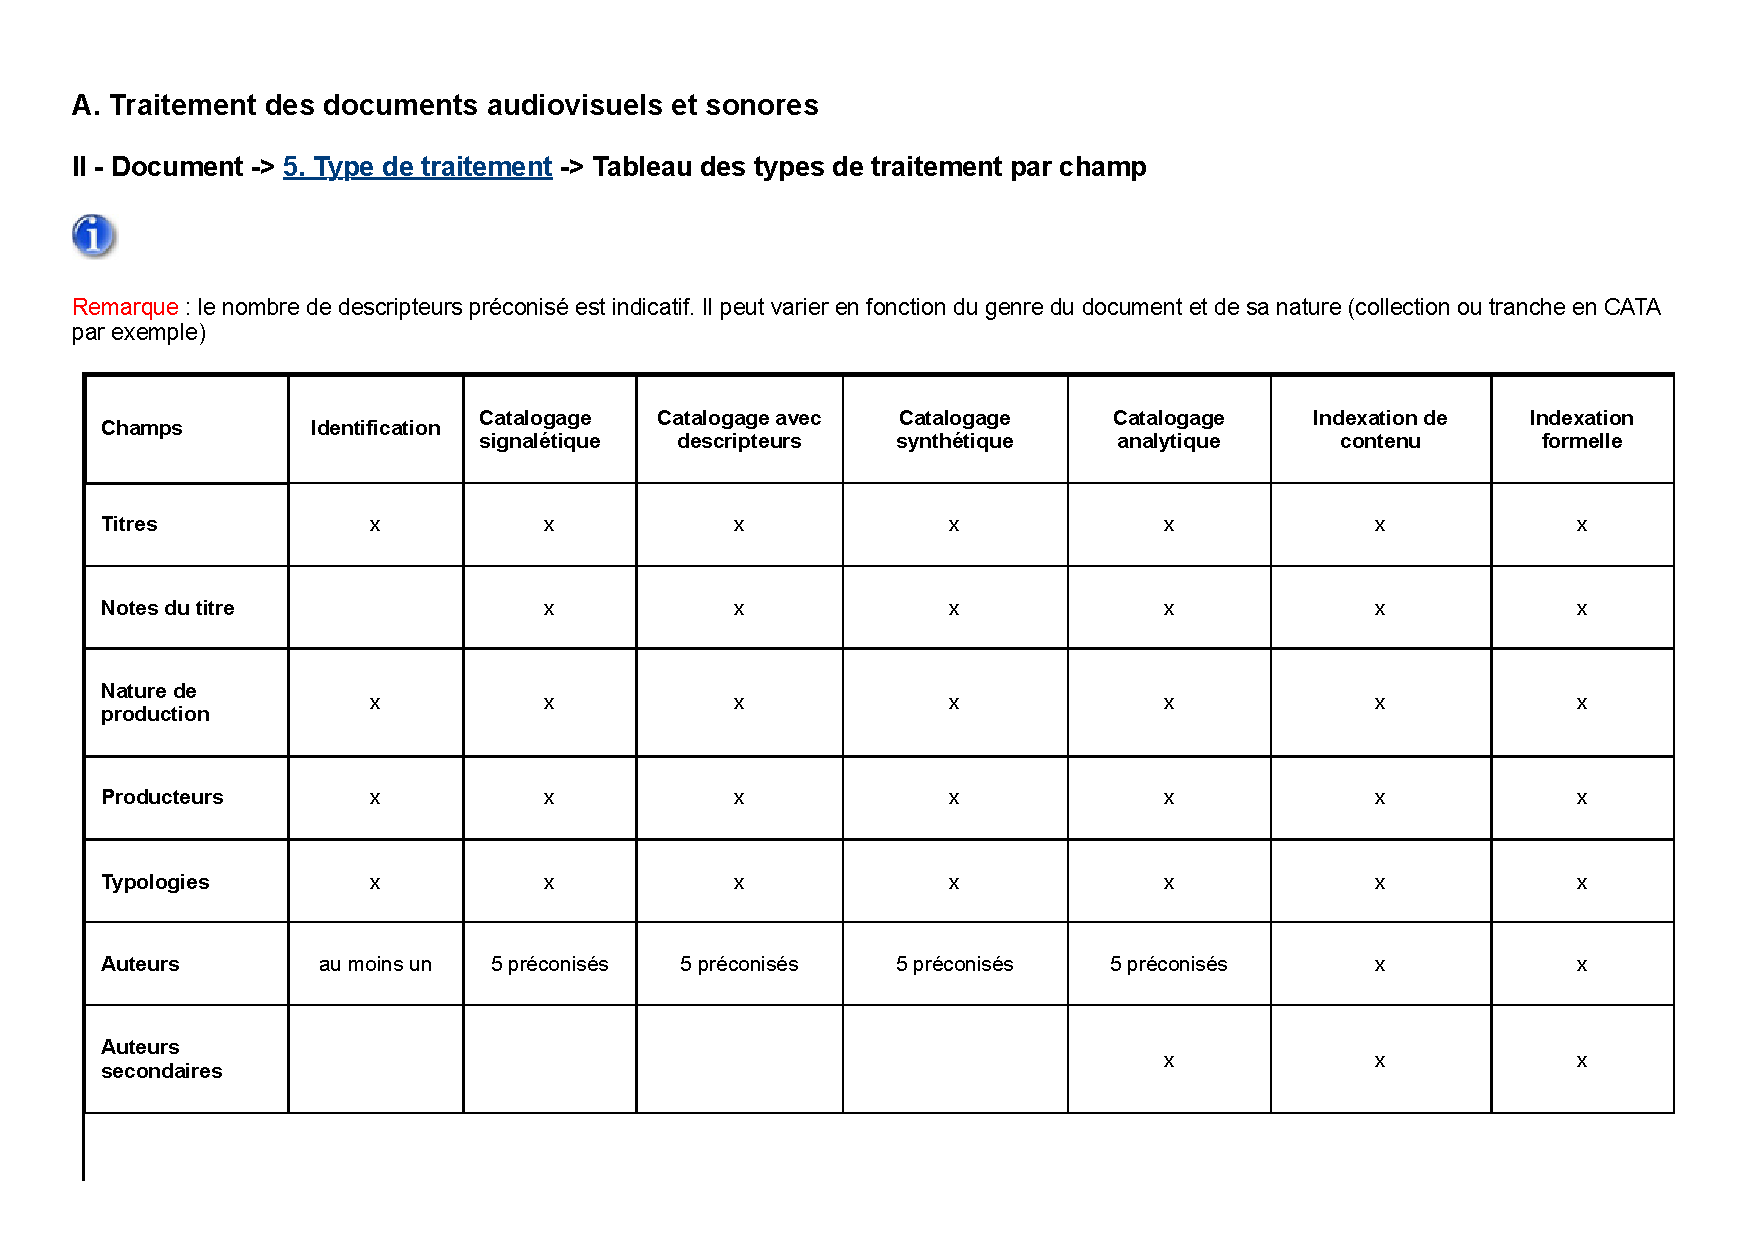
\includepdf[pages=-]{./illustrations/aidedl.pdf} 
	
	\chapter{Livrable : Cahier des charges du projet de cartographie du traitement documentaire}
	\label{ann:cdc}
	
	
\includepdf[pages=-]{./illustrations/cahier_charges_cartographie.pdf}
	
	\chapter{Organigramme de la direction des Patrimoines}
	\label{ann:org}
	
	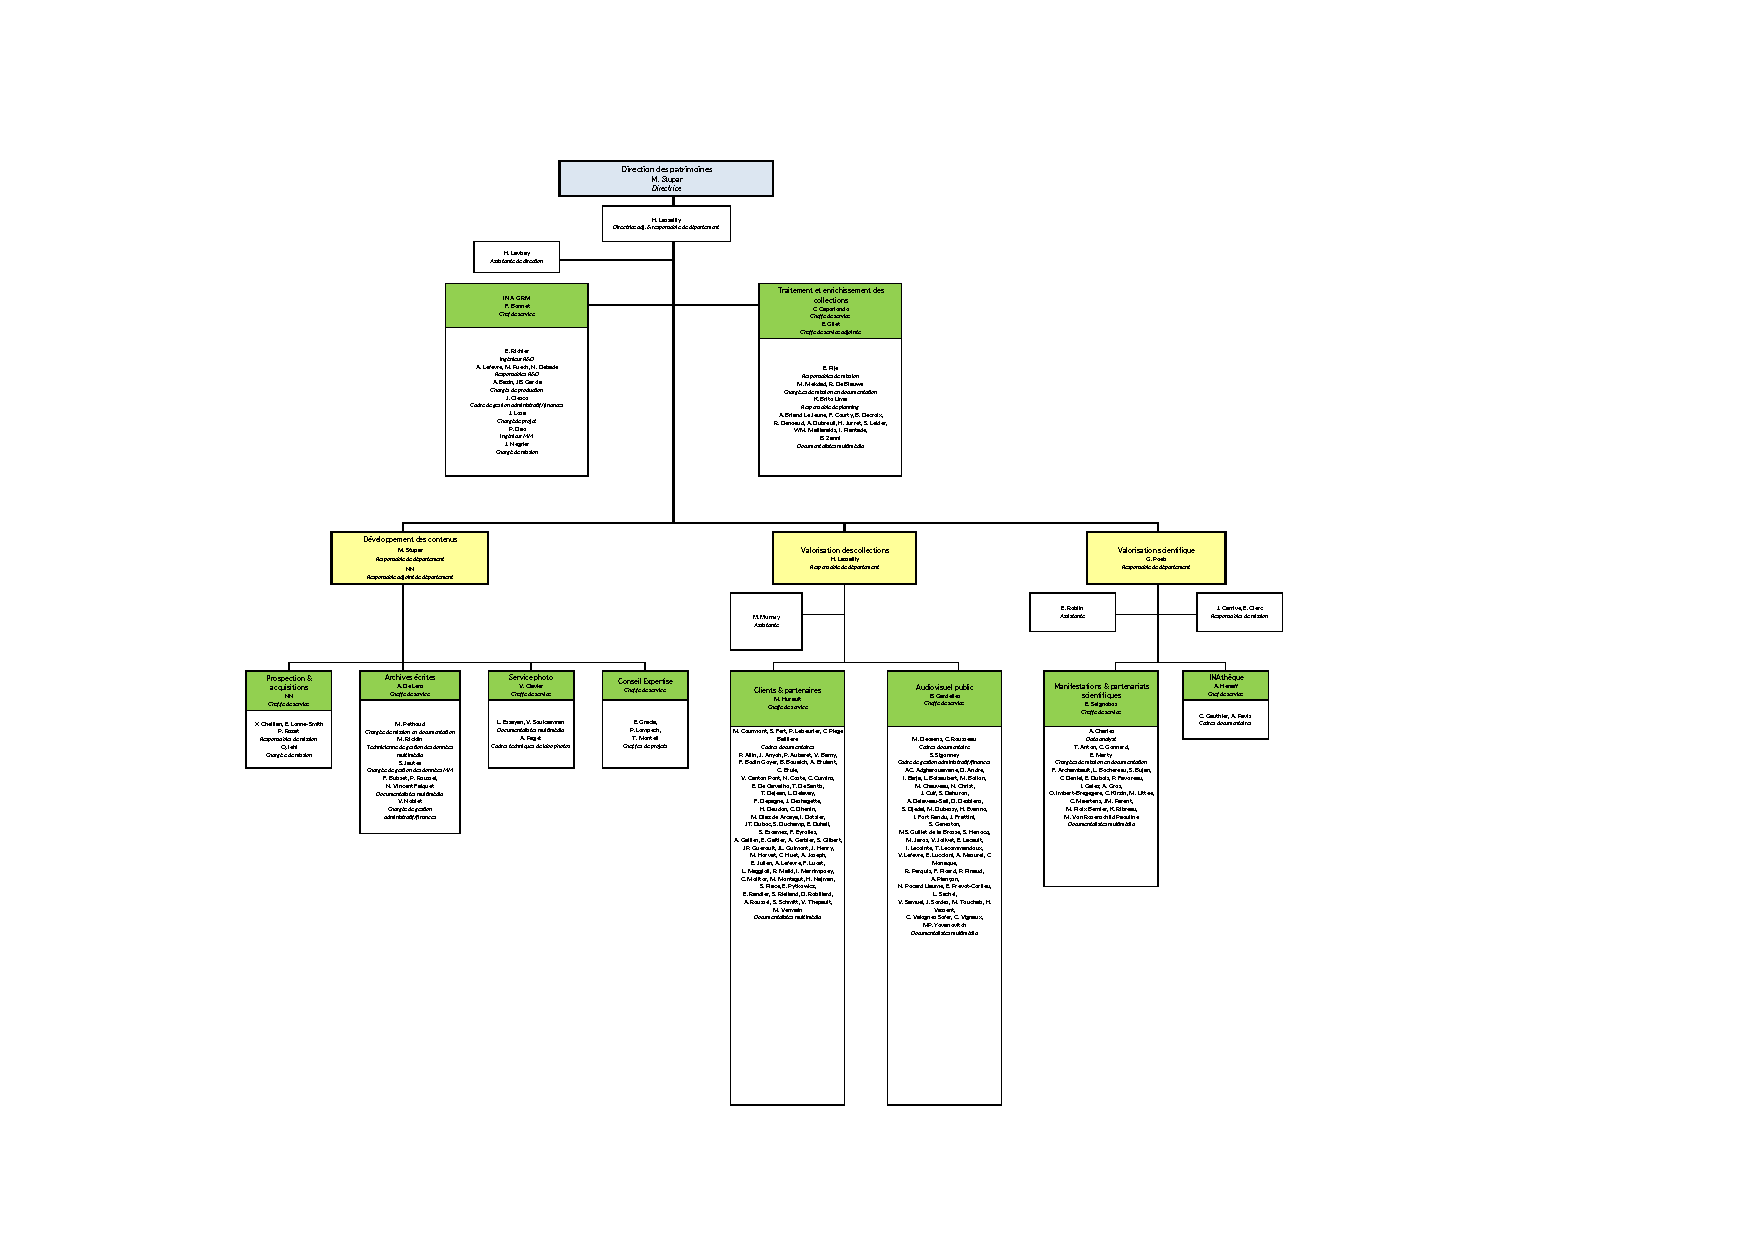
\includepdf[pages=-]{./illustrations/DP.pdf}
	
	\chapter{Notice de l'émission du 20H de TF1 du 14 juin 2024}
	\label{ann:notices}
	
		\section{Notice des archives professionnelles : Totem}
		
			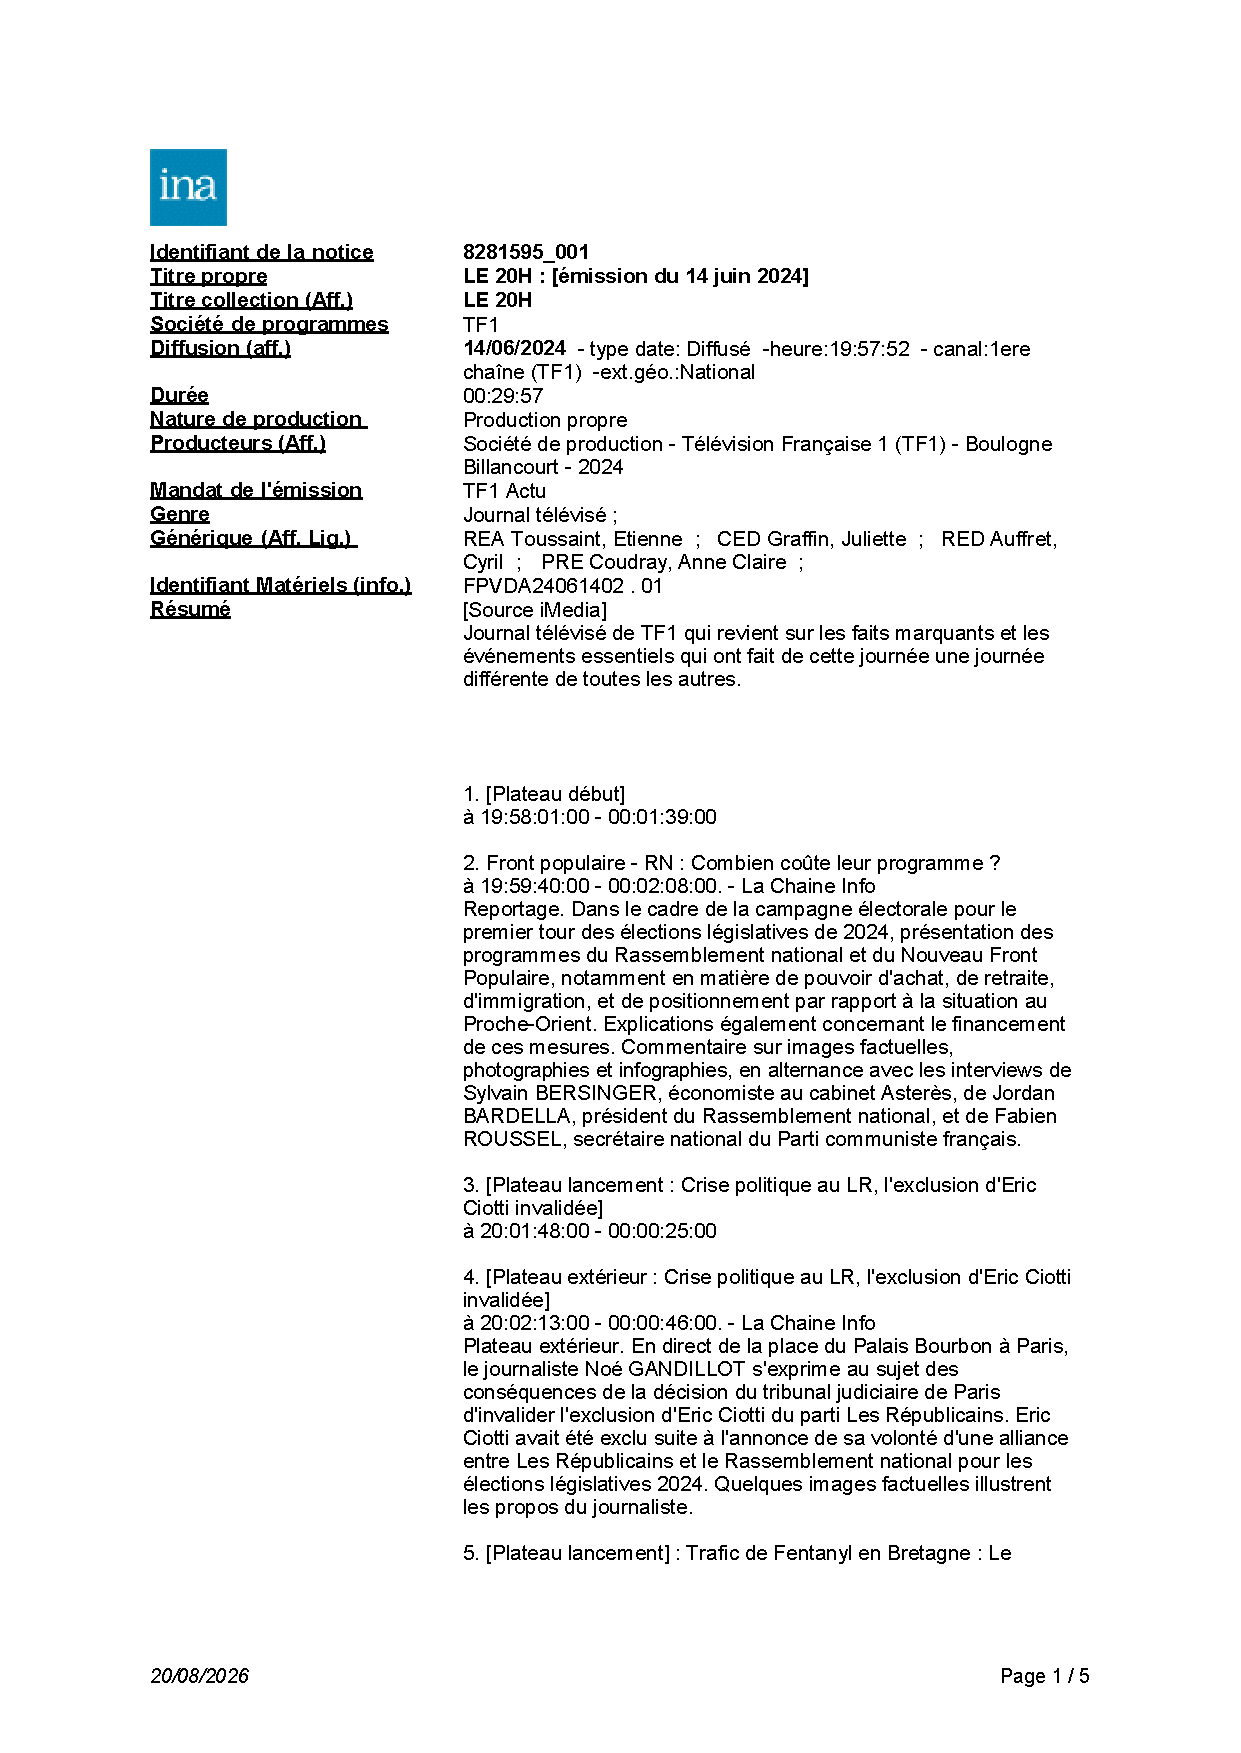
\includepdf[pages=-]{./illustrations/notice_14_juin_totem.pdf}
		
		\section{Notice du dépôt légal : Hyperbase}
		
			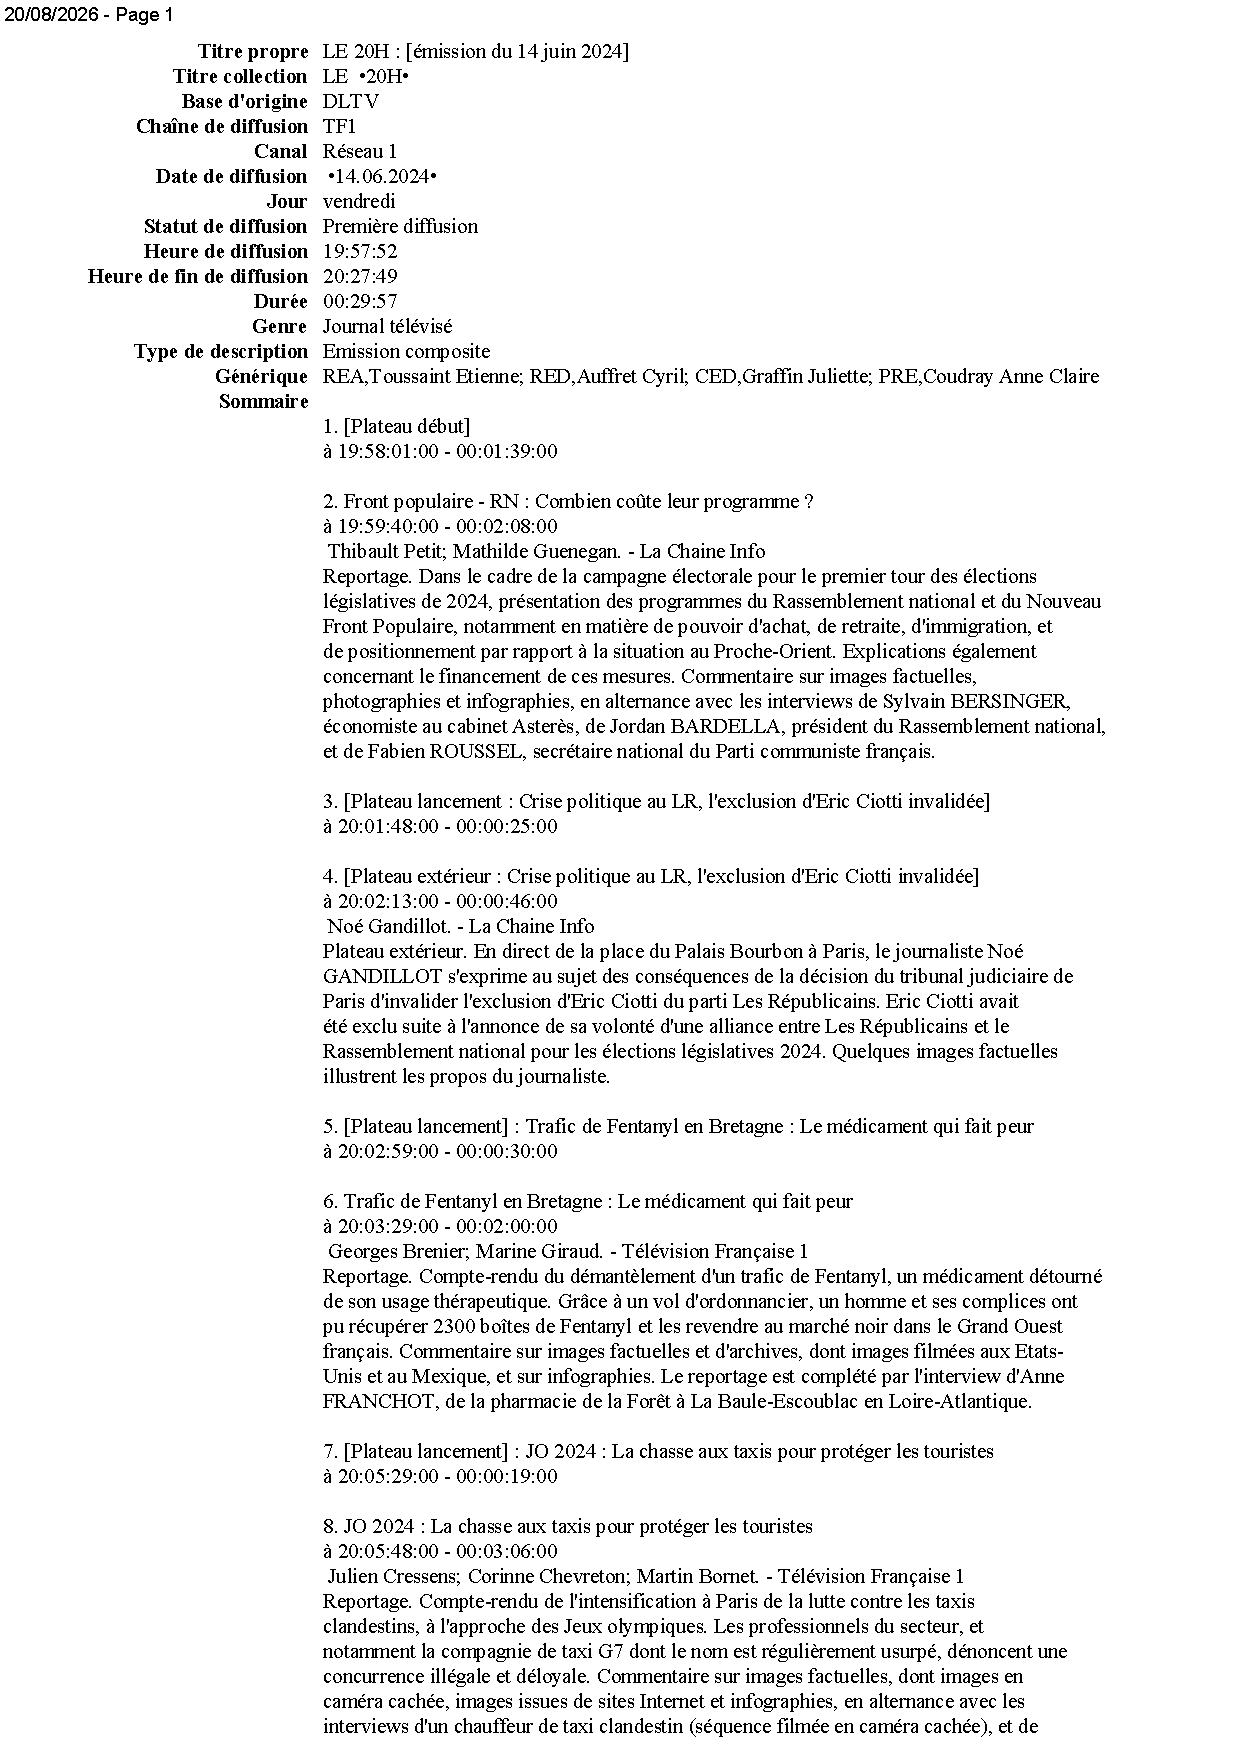
\includepdf[pages=-]{./illustrations/notice_14_juin_hyperbase.pdf}
	
	\let\addcontentsline\oldaddcontentsline

\newpage{\pagestyle{empty}\cleardoublepage}

%%%%%%%%%%%%%%%%%%

\backmatter % glossaire, index, table des figures, table des matières.. (la bibliographie a déjà été appelée)

%\printindex
%\printglossaries[title=Glossaire]
%\listoftables
%\listoffigures
\tableofcontents
\end{document}
